%Options: KBD=ISO8859; STD=VOID; LANG=FRENCH; FMT=latex; HYPHEN=default;
\documentclass[french,a4paper,12pt,twoside]{book}
\usepackage[french]{babel}
\usepackage[T1]{fontenc}
\usepackage[ansinew]{inputenc}
\usepackage{multicol,comment}
\usepackage{graphicx,color}
\usepackage{calrsfs}
\usepackage{macrosug}
\usepackage[hyperindex,colorlinks,linkcolor=blue,filecolor=blue,citecolor=red,pdfpagemode=None]{hyperref}
\topmargin-1cm
\textheight 25cm
\oddsidemargin-0.5cm
\evensidemargin-0.5cm
\textwidth17cm
\parindent0pt
\parskip2mm

\makeatletter
\def\logag{\incgr[width=1cm]{logoag.eps}}
\def\logstop{\incgr[width=0.75cm]{stop.eps}}
\def\fullscreen{\incgr[width=0.75cm]{HalfArrw.jpg}}
\def\loggsview{\incgr[width=0.75cm]{gsview.bmp}}
\def\rep{C\string:/Users/Utilisateur/Dropbox/Textes_AG/ModemploiAG2}

%\begin{comment}
\def\@hyper@launch run:#1\\#2#3{%
  \leavevmode
  \special{!aref
    <u=%
      /Type /Action
      /S /Launch
      /F (#1)
     \ifHy@newwindow /NewWindow true \fi
    \ifx\\#3\\\else /Win << /F (#1) /P (#3) >> \fi%
    >;%
    a=</Border [\@pdfborder] /C [\@runbordercolor]>%
  }%
  \Hy@colorlink{\@filecolor}#2\Hy@endcolorlink
  \special{!endaref}%
}
%\end{comment}

\def\BoutonAG#1{\fbox{\vbox to 1.5cm{\hbox to 1cm{\@hyper@launch %
run:{#1}\\{\logag}{}}\small\texttt{#1}\vss}}}

\def\BoutonStop{\vbox to 0.75cm{\hbox to 0.75cm{\hss\Acrobatmenu{Quit}{\logstop}\hss}\vss}\par}

\def\BoutonFS{\vbox to 0.75cm{\hbox to 0.75cm{\hss\Acrobatmenu{FullScreen}{\fullscreen}\hss}\vss}\par}

\def\BoutonGS#1{\vbox to 0.75cm{\hbox to 0.75cm{\hss\@hyper@launch run:{#1}\\{\loggsview}{}\hss}\vss}\par}
\makeatother

%% Pour les liens � la fois internes et externes, utiliser
%\hyperdef{category}{name}{text} et
% en interne: \hyperlink{category.name}{text}
% en externe: \hyperref{URL}{category}{name}{text}

\makeindex

\title{{\Huge\sffamily\bfseries Guide utilisateur du logiciel}\\[2cm]
{\Huge\color{red}\sffamily\bfseries Apprenti G�om�tre\\[2cm]
\color{black}\Large version 2.5.0}}

\author{\normalsize\baselineskip15pt Centre de Recherche sur l'Enseignement des Math�matiques\\}
\date{\today}


\bibliographystyle{plainn}

%\includeonly{chap12}

\begin{document}
\frontmatter
%\maketitle\newpage


\chapter*{Les modifications apport�es � \AG}


\section*{Version 2.5.0}\label{chapnouv5_0}                  Mis
� part une nouveaut� importante du point de vue technique, la
version 2.5.0 ne comporte que peu d'innovations d'ordre
fonctionnel. Commen�ons donc par le changement technique, lequel
devrait r�jouir presque tous ceux qui disposent d'un ordinateur
travaillant en 64 bits: {\sffamily\bfseries Apprenti G�om�tre}
existe d�sormais en deux versions, une version \og 32 bits\fg\
et une version \og 64 bits\fg. Pourquoi \og \textit{presque}
tous ceux\fg? Parce que, malheureusement, le compilateur que
nous utilisons, s'il nous fournit des versions 32 bits et 64
bits pour les ordinateurs fonctionnant sous \textit{Windows} ou
\textit{Linux}, ne nous fournit que la seule version 32 bits
pour les ordinateurs \textit{Macintosh}. Esp�rons que la version
64 bits soit r�alisable bient�t!

En ce qui concerne le logiciel lui-m�me, beaucoup de changements
ont permis d'am�liorer son fonctionnement sans n�cessiter un
nouvel apprentissage pour l'utilisateur. Il en est deux qui
n�cessitent plus de commentaires.

Le premier concerne l'introduction parmi les formes libres d'un
nouveau type d'objet g�om�trique: les secteurs de disque. Ils
sont accessibles � partir de l'un des menus C et AC. Les
secteurs de disque se manipulent essentiellement comme les arcs,
mais comme leur bord est une courbe ferm�e, il est possible d'en
colorier l'int�rieur, ce qui n'est pas possible avec un arc. Les
secteurs de disque font partie de la famille du cercle (voir au
chapitre 3).

Une autre innovation --- plus importante --- est la possibilit�
de rendre d�sormais la couleur de fond  d'une forme g�om�trique
semi-transparente. Si deux formes sont  colori�es en mode
semi-transparent, leur intersection �ventuelle est colori�e en
une troisi�me couleur sans qu'il soit n�cessaire de construitre
g�om�triquement la dite intersection. Par exemple, si deux
bandes colori�es en semi-transparence se croisent, leur
intersection est clairement visible sans qu'il soit n�cessaire
d'en construire le parall�logramme. De plus les modifications
induites par le d�placement d'une bande par rapport � l'autre
sont imm�diatement visibles.

Vous trouverez au chapitre 10 des figures permettant d'appr�cier
les diff�rences entre les modes \textit{Opaque,
Semi-transparent} et \textit{Transparent}.
 
\section*{Version 2.4.1}\label{chapnouv4_1}

La  plupart des modifications introduites dans cette version
2.4.1 sont des corrections d'erreurs ou de dysfonctionnements du
logiciel apparaissant lors de l'ex�cution de figures relativement
compliqu�es. Toutefois, une modification plus importante devrait
�tre appr�ci�e par les  utilisateurs dans des classes de
l'enseignement primaire: les formes standard ne sont d�sormais
plus mises sur le m�me pied que les formes libres pour ce qui
concerne l'orientation. Concr�tement cela signifie surtout que
l'aire d'une telle forme ne change plus de signe quand on la
retourne et que la fusion de deux formes standard est plus
simple que celle de deux formes libres. Pr�cisons qu'il reste
possible de fl�cher les c�t�s d'une forme standard de fa�on � en
montrer le sens de parcours.

\section*{Version 2.4.0}\label{chapnouv4_0}

Outre les corrections de bugs et modifications purement cosm�tiques, cette nouvelle version comporte des
innovations notables.

 \begin{itemize} \item L'innovation la plus importante consiste en l'introduction dans
le logiciel du concept de macro.  Une macro r�sulte de l'enregistrement d'une s�quence d'instructions, lesquelles peuvent elles-m�mes �tre des macros.
 Il en r�sulte l'adjonction au pr�sent guide d'un chapitre \ref{chapmac},
nouveau,  que  l'utilisateur voudra bien consulter attentivement.

\item L'utilisateur a d�sormais la possibilit� de convertir des formes libres en formes standard,  cr�ant
ainsi de nouvelles  familles de formes standard. � cet effet, il utilisera la fonctionnalit�
\texttt{Standardiser} du menu \textit{Fichiers}. Voir page \pageref{chapfstd.stdiser}.

\item Des transformations g�om�triques suppl�mentaires ont �t� introduites dans le menu
\hyperlink{chaptsf.Transformations}{\textit{Transformations}}.   Il s'agit  \begin{enumerate} \item des d�placements g�n�raux, c'est
� dire des rotations et translations d�finies � partir de deux points et de leurs images. Il n'est donc plus
n�cessaire de conna�tre ni le centre ni l'angle d'une rotation pour la construire. Cette nouvelle possibilit�
donnera � l'utilisateur la possibilit� de reporter des longueurs, d'un segment ou d'une droite sur un segment
ou une droite. Voir page \pageref{chaptsf.depla}.                              \item de deux types de transformations affines : les �tirements
et les cisaillements. Ces transformations permettent par exemple de construire une ellipse en tant qu'image
d'un cercle. Voir page \pageref{chaptsf.etir}.

 \end{enumerate}

\end{itemize}

\section*{Version 2.3.9}\label{chapnouv3_9}

\begin{itemize}
\item L'interface a �t� revu afin de permettre � l'utilisateur de modifier la taille des polices de caract�res utilis�es.

\item Le dessin et la gestion des cercles, arcs et formes hybrides ont �t� compl�tement r�vis�s. On ne peut cependant pas encore fusionner deux formes hybrides.


\item La routine de \hyperlink{chapoper.Fusionner}{fusion} des formes libres a �t� modifi�e de sorte que toute modification � une des deux formes fusionn�es ou au r�sultat de la fusion se
r�percute sur les deux autres formes. La fusion de deux polygones tient compte de l'orientation de ceux-ci.

\item La routine de construction d'un point d'intersection de deux formes a �t� am�lior�e dans le cas de deux segments superpos�s.

\item La routine d'\hyperlink{chapmouv.Ajustement}{ajustement} a �t� modifi�e de fa�on � faciliter la fusion de deux formes g�om�triques.

\item La \hyperlink{chapmodif.PtFix}{r�gle de choix} des points fixes lors de la modification d'une figure a �t� modifi�e.

\item Il est d�sormais possible d'augmenter ou diminuer le nombre de d�cimales affich�es pour les \hyperlink{chapoutils.Mesure}{longueurs et aires}.

\end{itemize}

\section*{Les versions 2.3.7 et 2.3.8}

La version 2.3.7 r�sulte de la conjonction de deux processus:

\begin{list}{\textbullet}{\itemsep=1mm}
\item Le premier processus  se r�alise en
permanence; il concerne l'am�lioration  des performances du logiciel. De ce point
de vue, nous pouvons citer pour la version 2.3.7

\begin{itemize}
\item la suppression d'erreurs de programmation, qui affectaient
principalement les  fonctionnalit�s \texttt{Annuler} et \texttt{Refaire}, ainsi
que la lecture d'un historique (qui utilise les m�mes m�thodes que
\texttt{Refaire}).

\item le remaniement de la routine qui gouverne les  modifications de figures, et �
ce titre constitue l'�l�ment central du logiciel. La nouvelle routine de
modification devrait permettre un dynamisme plus souple et provoquer moins de
blocages de figures que la pr�c�dente. � v�rifier\ldots

\item la r��criture des routines de gestion des figures hybrides. Le r�sultat
atteint est bon. Mais des difficult�s subsistent. Elles n�cessitent une
modification de la structure m�me d'une figure hybride. Ce sera --- peut-�tre ---
pour la prochaine version.
\end{itemize}
 
\item Le deuxi�me processus est l'introduction de nouvelles fonctionnalit�s.
La version 2.3.7 en comporte plusieurs.

\begin{itemize} \item L'op�ration \texttt{Dupliquer} permet d�sormais de dupliquer
un \og point sur\fg\ un segment vers un cercle ou un arc de cercle.

\item Un \og point sur\fg\ un arc de cercle peut �tre anim�, via le menu
contextuel.

\item Un \og point sur\fg\ un polygone peut �tre astreint � rester sur un c�t�. Il
n'a donc plus acc�s � l'int�gralit� du polygone. La commande \texttt{Limiter au
c�t�} a �t� introduite � cet effet dans le menu contextuel.
\end{itemize}

\item Il est d�sormais possible de cacher une transformation g�om�trique, sans
cacher son support.

\item Enfin, � partir du menu \texttt{Pr�f�rences}, il est d�sormais possible
de changer les unit�s de longueur et d'aire utilis�es pour
l'affichage des mesures correspondantes.
 
\end{list}

La version 2.3.8  diff�re de la version 2.3.7 essentiellement par la correction d'une erreur de
programmation qui entra�nait dses d�formations intempestives de certaines figures lors d'un mouvement.
Quelques autres am�liorations portent sur la gestion des points d'intersection et des formes conditionn�es.





%Options: KBD=VOID; STD=VOID; LANG=FRENCH; FMT=LATEXL1; HYPHEN=DEFAULT;
\fbox{\begin{minipage}[c][0.99\textheight][c]{0.99\linewidth}
\begin{center}
\Large\bfseries Avant-propos
\end{center}

\leftskip 0.5cm \rightskip 0.5cm

La premi�re version du logiciel \AG\ est apparue en 2003, pour r�pondre au
d�sir du Ministre de l'Enseignement fondamental Jean-Marc \textsc{Nollet} de mettre � la disposition des
�l�ves d'�cole primaire un logiciel  leur permettant de r�aliser des activit�s g�om�triques intuitives,
bas�es notamment sur l'emploi de \og mouvements\fg. Le ministre chargea le \textsc{crem}
de concevoir ce logiciel et en confia la r�alisation � une firme priv�e.

D�s le d�part, les responsables du \textsc{crem} estim�rent que --- dans une
optique de continuit� entre l'enseignement fondamental et l'enseignement
secondaire --- le logiciel devait �tre compl�t� de quelques fonctionnalit�s
simples accessibles tant � la fin de l'�cole primaire qu'au d�but du secondaire.
De l� naquit une organisation d'\AG\ {\sffamily\bfseries 1} en deux \og kits\fg:
un \og kit standard\fg\ comportant des formes ind�formables qui peuvent �tre
d�plac�es, d�coup�es, fusionn�es\ldots\ et un \og kit libre\fg\ comportant des
formes g�om�triques \og classiques\fg, triangles quelconques, rectangles,
isoc�les\ldots\ pouvant �tre d�form�es � volont�, ainsi que des points et des
segments mais pas d'objets \og illimit�s\fg\ tels que des droites ou bandes.

Les exp�rimentations r�alis�es � partir de 2003 montr�rent l'int�r�t du logiciel
tant dans l'enseignement primaire que dans les premi�res ann�es de
l'enseignement secondaire et encourag�rent les responsables du \textsc{crem} �
compl�ter le \og kit libre\fg\ par des fonctionnalit�s plus �labor�es
fournissant aux �l�ves du secondaire plus de possibilit�s dans le cadre
d'activit�s de r�solution de probl�mes. La deuxi�me version d'\AG\ qui en
r�sulta --- connue sous le nom d'\AG\ {\sffamily\bfseries 2} --- a �t� r�alis�e
sans aide officielle et uniquement gr�ce aux moyens humains et mat�riels du
\textsc{crem}. Elle a �t�  mise � disposition des �l�ves et des enseignants �
partir de janvier 2008. Elle incorpore des objets \og illimit�s\fg\  et augmente
consid�rablement les possibilit�s d'utiliser des transformations g�om�triques
(translations, sym�tries, rotations, homoth�ties et similitudes). Depuis lors,
elle a connu de nombreuses corrections et am�liorations, qui ont abouti � la
version 2.3.5 actuelle.

La version 2 est fid�le � la version 1. On y retrouve donc le \og kit standard\fg\ et le \og kit libre\fg, quoique sous de
nouveaux noms, � savoir le \og Menu A\fg\ et le \og Menu B\fg. Les fonctionnalit�s nouvelles par rapport � la version 1
figurent pour la plupart dans une extension du \og Menu B\fg\ d�nomm�e \og Menu C\fg. Cette r�partition en
trois menus permet de d�limiter l'utilisation d'\AG\ du d�but de l'�cole primaire � la fin du secondaire.

La conception de la version 1 d'\AG\ a �t� l'\oe uvre d'une �quipe du \textsc{crem} dirig�e par Nicolas
\textsc{Rouche} et comportant �galement Michel \textsc{Ballieu}, Marie-France \textsc{Guissard} et
Marie-Fran�oise \textsc{Van Troeye}. Les premi�res exp�rimentations de cette version ont �t� r�alis�es par
Marie-Fran�oise \textsc{Van Troeye} et Philippe \textsc{Skilbecq}.

La version 2 a �t� concue et r�alis�e par une �quipe dirig�e par Guy \textsc{No�l} et comprenant �galement
Bernard \textsc{Honclaire} pour la conception et Geoffrey \textsc{Pliez} pour la programmation. Elle a �t�
exp�riment�e par Philippe \textsc{Skilbecq} et Andr� \textsc{Vandenbruaene} lors d'une recherche du
\textsc{crem}, men�e de 2005 � 2007, � laquelle participaient de plus S�bastien \textsc{Agie}, Pierrette
\textsc{De Rijck}, Michel \textsc{Herman}, Philippe \textsc{Mairesse} et Gregory \textsc{Philippart}.

Une premi�re version du guide utilisateur a �t� r�dig�e par S�bastien \textsc{Agie}, Pauline
\textsc{Lambrecht} et Guy \textsc{No�l}.  La pr�sente version r�sulte de remaniements et de compl�ments
apport�s � la  premi�re version par Guy \textsc{No�l}.

\end{minipage} }
%\tableofcontents
\mainmatter
\include{chap1}   %chapintro
%%%%%%%%%%%%%%%%%%%%%%%%%%%%%%%%%%%%%%%%%%%%%%%%%%%%%%%%%%%%%%%%%%%%%%%
\chapter{Les formes standard}

\label{chapfstd}
\section{Introduction}

Les formes \textit{standard}\index{Forme!standard} sont des formes g�om�triques ind�formables, ce qui
les distingue des  formes \textit{libres}\index{Forme!libre} qui seront d�crites au chapitre
\ref{chapflib}. Les fonctionnalit�s --- largement communes aux formes standard et aux formes libres ---
qui permettent de  manipuler ces formes seront d�crites aux chapitres suivants. Les formes standard
sont accessibles � partir de l'un des menus A, AB ou AC.
Apr�s que l'utilisateur ait s�lectionn� un de ces menus, une fen�tre s'ouvre, comportant en haut une barre de
\textit{menus} o� figurent notamment des \textit{outils} et des \textit{op�rations}\medskip

\centerline{\includegraphics[width=0.6\linewidth]{MenuA.bmp}}
\leg{}

Sur la gauche de l'�cran appara�t une \textit{bo�te � outils} avec un \textit{pav� de mouvements} et un
\textit{pav� de formes standard}\footnote{Les illustrations du pr�sent fascicule sont conformes aux �crans
qui apparaissaient \textsc{avant} la version 2.3.6.}.  Le reste de  l'�cran constitue la \textit{fen�tre de
dessin} o� une \textit{figure} sera construite.
\index{Menu}\index{Outil}\index{Operation@Op�ration}\index{Mouvement} \index{Forme!standard} Les touches
\fbox{+}, \fbox{-} et \fbox{=} permettent de modifier la taille des caract�res des textes affich�s sur les
diff�rents boutons (mais pas ceux de la barre des menus).

Par d�faut, les formes standard sont celles du \textit{jeu de base}\index{Jeu! de base}. D'autres
jeux de formes standard peuvent �tre choisis via l'item \textit{Pr�f�rences} (voir le paragraphe \ref{autresjeux}).

\section{Construire une forme standard}

Un jeu de formes standard est constitu� d'une ou plusieurs \textit{familles}\index{Famille} de formes.
Chaque famille est accessible via une ic�ne affich�e dans le pav� de formes standard de la bo�te �
outils. Un clic sur une de ces ic�nes fait appara�tre une fen�tre comportant autant de boutons-poussoirs
qu'il y a de formes dans la famille s�lectionn�e. Ces boutons permettent de choisir la forme qui sera
dessin�e.

Le dessin d'une forme standard est compl�tement d�termin� par la fixation d'un point, appel� le \og
point de r�f�rence\fg\ de la forme. Il s'agit g�n�ralement (mais pas toujours) du sommet \og
inf�rieur-gauche\fg.
\index{Point!de r�f�rence}\bigskip

\danger\hfill \fbox{\begin{minipage}{0.87\linewidth} \label{doubleclic} Lors de la construction
d'une forme g�om�trique, il peut arriver que l'utilisateur r�alise involontairement un \og
\hyperdef{chapfstd}{doubleclic}{double clic}\fg. En d'autres termes, il clique deux fois dans un
intervalle de temps tr�s court et en deux points tr�s proches l'un de l'autre, ce qui peut fausser
sa construction.\index{Double clic} L'ordinateur est programm� de mani�re � consid�rer comme double
clic deux clics distants de moins d'un dixi�me de seconde et en des positions distantes de
moins  de 5 pixels. Dans ce cas, il affiche un message ad�quat et annule le deuxi�me
clic.\end{minipage}}

\newpage

%\includegraphics[width=0.6\linewidth]{MenuA.bmp}\\
\fbox{\begin{minipage}[b]{1.45cm}
\includegraphics[width=1.45cm]{Pavstandard2.bmp}
\leg{}\end{minipage}\begin{minipage}[b][12.5\baselineskip][c]{0.9\linewidth}\small \Prat
\begin{list}{\textbullet}{\itemsep=0mm}  \item S�lectionner une des familles du jeu de formes utilis� en
cliquant sur l'ic�ne symbole de cette famille.   \item Le clic fait appara�tre une fen�tre de boutons
poussoirs, un pour chaque forme de la famille. Quand le curseur de la souris survole un bouton de cette
fen�tre, l'ic�ne symbole de la famille est remplac�e par l'ic�ne repr�sentant la forme correspondant au
bouton survol�. \item S�lectionner une des formes de la famille en cliquant sur le bouton-poussoir
correspondant. Le curseur de la souris prend la forme d'une croix.\item Cliquer dans la fen�tre de
dessin: la forme s�lectionn�e est dessin�e, son point de r�f�rence est plac� � l'emplacement du clic.
\item Tout clic suppl�mentaire dans la fen�tre de dessin fait appara�tre un exemplaire suppl�mentaire
de la forme s�lectionn�e. \end{list}\vspace{\baselineskip} \end{minipage}}


\danger  \hfill
\fbox{\begin{minipage}{0.87\linewidth}\small   Si l'utilisateur entreprend de construire une forme standard alors que
d'autres formes (standard ou non) sont d�j� dessin�es � l'�cran, chaque fois que le curseur de la souris s'approche d'un
point existant � une distance inf�rieure � la distance de magn�tisme\index{Distance!de magn�tisme}, la couleur de  celui-ci
vire au magenta et le message affich� devient \og ce point ?\fg. \medskip
\begin{minipage}[b]{2cm}
\includegraphics[width=2cm]{cepoint.bmp}
\leg{}
\end{minipage}\begin{minipage}[b]{0.86\linewidth}
Si le clic est effectu� � ce moment, le point
de r�f�rence de la nouvelle forme est identifi� au point d�j� existant et les deux formes ont  un
sommet commun.%\vspace{0.5\baselineskip}
\end{minipage}
\end{minipage}}
 



\section{Le jeu de base}
\index{Jeu!de base}
 
Le jeu de base comprend trois familles de formes, chacune d�sign�e par le  nom d'un polygone r�gulier et
symbolis�e par l'ic�ne correspondante.  Deux principes ont gouvern� la construction de ces familles:

\begin{itemize}
\item chaque famille comporte un nombre limit� de formes simples et ind�formables ;
\item les formes d'une m�me famille ont entre elles des rapports simples de
longueurs, d'angles et d'aires, de sorte qu'en les d�coupant, assemblant et
fusionnant, il est possible de r�aliser de nombreuses autres formes ou combinaisons
g�om�triques int�ressantes.
\end{itemize}


\subsection{La famille du triangle �quilat�ral}

\fbox{\begin{minipage}{0.99\linewidth}
La famille du triangle �quilat�ral comporte douze �l�ments:

\begin{minipage}{0.6\linewidth}
\centerline{\includegraphics[width=0.7\linewidth]{Famtriequi.eps}}
\leg{\label{Famtriequi.eps}}
\end{minipage}
\hfill
\begin{minipage}{0.4\linewidth}
\centerline{\includegraphics[width=0.75\linewidth]{Famtriequi_menu.bmp}}
\leg{\label{Famtriequi_menu.jpg}}
\end{minipage}
\end{minipage}}



\multicolsep 0pt \begin{multicols}{2}
\begin{minipage}[b]{0.35\linewidth}\begin{center}\includeg{0.4\linewidth}
{0.75\linewidth}{TriEqui.eps}\end{center} \end{minipage}\hfill \begin{minipage}{0.68\linewidth}un
triangle �quilat�ral\index{Triangle!�quilat�ral}, symbole de la famille; \end{minipage}

\begin{minipage}[b]{0.35\linewidth}\begin{center}\includeg{0.4\linewidth}
{0.75\linewidth}{Losange_TrA.eps}\end{center} \end{minipage}\hfill
\begin{minipage}{0.68\linewidth}un losange\index{Losange} form� de deux de ces triangles;
\end{minipage}

\begin{minipage}[b]{0.35\linewidth}\begin{center}\includeg{0.4\linewidth}
{0.75\linewidth}{Trapiso_TrA.eps}\end{center} \end{minipage}\hfill
\begin{minipage}{0.68\linewidth}un trap�ze isoc�le\index{Trap�ze!isoc�le} form� � partir de
trois de ces triangles;         \end{minipage}

\begin{minipage}[b]{0.35\linewidth}\begin{center}\includeg{0.4\linewidth}
{0.75\linewidth}{Hexagone_TrA.eps}\end{center} \end{minipage}\hfill
\begin{minipage}{0.68\linewidth}un hexagone r�gulier\index{Hexagone!r�gulier} form� � partir de six
de ces triangles;         \end{minipage}


\begin{minipage}[b]{0.35\linewidth}\begin{center}\includeg{0.45\linewidth}
{0.75\linewidth}{PtTriso_TrA.eps}\end{center} \end{minipage}\hfill
\begin{minipage}{0.68\linewidth}un
triangle isoc�le\index{Triangle!isoc�le} tiers du triangle �quilat�ral;         \end{minipage}

\begin{minipage}[b]{0.35\linewidth}\begin{center}\includeg{0.45\linewidth}
{0.75\linewidth}{Trirect_TrA.eps}\end{center} \end{minipage}\hfill
\begin{minipage}{0.68\linewidth}un
triangle rectangle\index{Triangle!rectangle} moiti� du triangle �quilat�ral;           \end{minipage}

\begin{minipage}[b]{0.35\linewidth}\begin{center}\includeg{0.45\linewidth}
{0.75\linewidth}{Traprect_TrA.eps}\end{center} \end{minipage}\hfill
\begin{minipage}{0.68\linewidth} un trap�ze rectangle\index{Trap�ze!rectangle} assemblage de trois
de ces triangles rectangles;  \end{minipage}

\begin{minipage}[b]{0.35\linewidth}\begin{center}\includeg{0.45\linewidth}
{0.75\linewidth}{Dodecagone_TrA.eps}\end{center} \end{minipage}\hfill
\begin{minipage}{0.68\linewidth}un dod�cagone\index{Dod�cagone} r�gulier ayant m�me c�t� que le
triangle �quilat�ral; \end{minipage}

\begin{minipage}[b]{0.35\linewidth}\begin{center}\includeg{0.45\linewidth}
{0.75\linewidth}{GrTriso_TrA.eps}\end{center} \end{minipage}\hfill \begin{minipage}{0.68\linewidth} un
grand triangle isoc�le\index{Triangle!isoc�le} qui permet de paver le dod�cagone; \end{minipage}

\begin{minipage}[b]{0.35\linewidth}\begin{center}\includeg{0.45\linewidth}
{0.75\linewidth}{Rosacepetitlos.eps}\end{center} \end{minipage}\hfill \begin{minipage}{0.68\linewidth} un petit
losange\index{Losange} d�termin� par trois sommets cons�cutifs du dod�cagone;\end{minipage}

\begin{minipage}[b]{0.35\linewidth}\begin{center}\includeg{0.45\linewidth}
{0.75\linewidth}{Petitcercle_TrA.eps}\end{center} \end{minipage}\hfill
\begin{minipage}{0.68\linewidth} un petit disque\index{Disque} dans lequel on peut inscrire
un triangle �quilat�ral ; \end{minipage}

\begin{minipage}[b]{0.35\linewidth}\begin{center}\includeg{0.45\linewidth}
{0.75\linewidth}{Grandcercle_TrA.eps}\end{center} \end{minipage}\hfill
\begin{minipage}{0.6\linewidth} et un grand disque\index{Disque} dans lequel on peut
inscrire  l'hexagone et le grand triangle isoc�le.\end{minipage}
\end{multicols}

\subsection{La famille du carr�}

\fbox{\begin{minipage}{0.99\linewidth}
La famille du carr� comporte neuf �l�ments:

\begin{minipage}{0.6\linewidth}
\centerline{\includegraphics[width=0.45\linewidth]{Famcar.eps}}
\leg{\label{Famcar.eps}}
\end{minipage} \hfill
\begin{minipage}{0.4\linewidth}
\centerline{\includegraphics[width=0.75\linewidth]{Famcar_menu.bmp}}
\leg{\label{Famcar_menu.jpg}}
\end{minipage}
\end{minipage}}


\begin{multicols}{2}
\begin{minipage}{0.45\linewidth}\begin{center}\includeg{0.35\linewidth}
{0.75\linewidth}{Carre.eps}\end{center} \end{minipage}\hfill
\begin{minipage}{0.58\linewidth}un carr�\index{Carre@Carr�}, symbole de la famille;
\end{minipage}


\begin{minipage}{0.45\linewidth}\begin{center}\includeg{0.35\linewidth}
{0.75\linewidth}{Trireciso_CarA.eps}\end{center} \end{minipage}\hfill
\begin{minipage}{0.58\linewidth}un triangle rectangle isoc�le\index{Triangle!rectangle isoc�le} moiti� du carr�;
\end{minipage}


\begin{minipage}{0.45\linewidth}\begin{center}\includeg{0.85\linewidth}
{0.25\linewidth}{Para_CarA.eps}\end{center} \end{minipage}\hfill
\begin{minipage}{0.58\linewidth}un parall�logramme\index{Parall�logramme} double du triangle ci-dessus;
\end{minipage}


\begin{minipage}{0.45\linewidth}\begin{center}\includeg{0.35\linewidth}
{0.75\linewidth}{Octo_CarA.eps}\end{center} \end{minipage}\hfill
\begin{minipage}{0.58\linewidth}un octogone r�gulier\index{Octogone} ayant m�me c�t� que le
carr� de r�f�rence;
\end{minipage}

\begin{minipage}{0.45\linewidth}\begin{center}\includeg{0.35\linewidth}
{0.75\linewidth}{Triso_CarA.eps}\end{center} \end{minipage}\hfill
\begin{minipage}{0.58\linewidth}un triangle isoc�le\index{Triangle!isoc�le} huiti�me de
l'octogone; \end{minipage}


\begin{minipage}{0.45\linewidth}\begin{center}\includeg{0.35\linewidth}
{0.75\linewidth}{PtTrireciso_CarA.eps}\end{center} \end{minipage}\hfill
\begin{minipage}{0.58\linewidth}un petit triangle rectangle isoc�le\index{Triangle!rectangle isoc�le}
quart du carr�;
\end{minipage}


\begin{minipage}{0.45\linewidth}\begin{center}\includeg{0.35\linewidth}
{0.75\linewidth}{PtTrirect_CarA.eps}\end{center} \end{minipage}\hfill
\begin{minipage}{0.58\linewidth}un petit triangle rectangle\index{Triangle!rectangle} �galement quart du carr�;
\end{minipage}


\begin{minipage}{0.45\linewidth}\begin{center}\includeg{0.35\linewidth}
{0.75\linewidth}{Petitlosange_CarA.eps}\end{center}
\end{minipage}\hfill \begin{minipage}{0.58\linewidth}un
losange\index{Losange} d�termin� par trois sommets
cons�cutifs  de l'octogone; \end{minipage}
\end{multicols}

\centerline{\begin{minipage}[b]{0.5\linewidth}
\begin{minipage}{0.45\linewidth}\begin{center}\includeg{0.35\linewidth}
{0.75\linewidth}{Cercle_CarA.eps}\end{center} \end{minipage}\hfill
\begin{minipage}{0.54\linewidth}et, enfin, un disque\index{Disque} dans lequel
on peut inscrire le carr� de r�f�rence. \end{minipage}\end{minipage}}



\subsection{La famille du pentagone}

\fbox{\begin{minipage}{\linewidth}
La famille du pentagone comporte sept �l�ments:

\begin{minipage}{0.5\linewidth}\begin{center}\includeg{0.9\linewidth}
{0.7\linewidth}{Fampentag.eps}\end{center}\end{minipage} \hfill
\begin{minipage}{0.5\linewidth}
\centerline{\includeg{0.8\linewidth}{0.7\linewidth}{Fampentag_menu.bmp}}
\vspace{0.3cm}
\end{minipage}
\end{minipage}}
\newpage


\begin{multicols}{2}
\begin{minipage}{0.45\linewidth}\begin{center}\includeg{0.35\linewidth}
{0.75\linewidth}{Pentagone.eps}\end{center} \end{minipage}\hfill
\begin{minipage}{0.58\linewidth} un  pentagone r�gulier\index{Pentagone}, symbole de la famille;
\end{minipage}

\begin{minipage}{0.45\linewidth}\begin{center}\includeg{0.35\linewidth}
{0.75\linewidth}{PtTriso_PentA.eps}\end{center} \end{minipage}\hfill
\begin{minipage}{0.58\linewidth}un  triangle isoc�le\index{Triangle!isoc�le}, cinqui�me du pentagone;
\end{minipage}


\begin{minipage}{0.45\linewidth}\begin{center}\includeg{0.35\linewidth}
{0.75\linewidth}{Decag.eps}\end{center} \end{minipage}\hfill
\begin{minipage}{0.58\linewidth}un d�cagone\index{Decagone@D�cagone} r�gulier ayant m�me c�t� que le
pentagone r�gulier;         \end{minipage}


\begin{minipage}{0.45\linewidth}\begin{center}\includeg{0.35\linewidth}
{0.75\linewidth}{GrTriso_PentA.eps}\end{center} \end{minipage}\hfill
\begin{minipage}{0.58\linewidth}un grand triangle isoc�le\index{Triangle!isoc�le}, dixi�me du d�cagone;
\end{minipage}

\begin{minipage}{0.45\linewidth}\begin{center}\includeg{0.5\linewidth}
{0.5\linewidth}{Trisobtus_PentA.eps}\end{center}\end{minipage}
\begin{minipage}{0.58\linewidth} un triangle obtusangle\index{Triangle!obtusangle}
apparaissant dans le pavage du pentagone; \end{minipage}

\begin{minipage}{0.45\linewidth}\begin{center}\includeg{0.35\linewidth}
{0.75\linewidth}{Petitlospenta.eps}\end{center}
\end{minipage}\hfill \begin{minipage}{0.58\linewidth}un
petit losange\index{Losange} d�termin� par trois sommets
cons�cutifs du d�cagone; \end{minipage}
\end{multicols}

\centerline{\begin{minipage}[b]{0.5\linewidth}
\begin{minipage}{0.45\linewidth}\begin{center}\includeg{0.35\linewidth}
{0.75\linewidth}{Cercle_PentA.eps}\end{center} \end{minipage}\hfill
\begin{minipage}{0.54\linewidth}et, enfin, un disque\index{Disque} dans lequel on peut inscrire un
pentagone. \end{minipage}\end{minipage}}


\section{Les formes standard: quelques options}\label{autresjeux}

Via le menu \texttt{Pr�f�rences/Formes standard}\index{Forme!standard}, il est
possible de modifier certaines caract�ristiques des formes standard.

\begin{description} \item[Remplacer le jeu de base par un autre jeu de formes standard]\index{Jeu!de
formes standard}\strut

 En plus du jeu de base, le programme d'installation d'\AG\ 2 enregistre sur le disque dur plusieurs
fichiers  (d'extension \texttt{.std}\index{.std@\texttt{.std}}) comportant des formes
manipulables de la m�me mani�re que celles du jeu de base.

\begin{list}{\textbullet}{\itemsep=1mm}

\item \texttt{Jeu r�duit} ne contient qu'un sous-ensemble des pi�ces du jeu de
base: neuf formes de la famille du triangle �quilat�ral, six formes de la famille du carr� et six
formes de la famille du pentagone r�gulier. Ce jeu peut �tre utilis� pour des activit�s
�l�mentaires.\index{Jeu!r�duit}

\item \texttt{Polyminos} propose quatre familles de formes. La premi�re est limit�e � un
carr� et un rectangle $1\times 2$ (un \og domino\fg). La deuxi�me contient les deux
triminos, la troisi�me contient  les cinq quadriminos et enfin, la quatri�me contient
les douze pentaminos, donnant ainsi acc�s � une s�rie de puzzles bien
connus.\index{Domino}\index{Trimino}\index{Quadrimino}\index{Pentamino}\index{Polymino}

\begin{center}
\includegraphics[width=0.45\linewidth]{polyminos1.eps}

\leg{\label{polyminos1}}

\includegraphics[width=0.9\linewidth]{polyminos2.eps}

\leg{\label{polyminos2}}
\end{center}

\item \texttt{Tangram}\index{Tangram} est un autre jeu tout aussi c�l�bre.\medskip

\begin{minipage}[b]{0.2\linewidth}
\includegraphics[width=\linewidth]{tangram.eps}

\leg{\label{Tangram}}
\end{minipage}
\hfill
\begin{minipage}[b]{0.7\linewidth}

La famille du Tangram ne contient que cinq pi�ces:
\begin{itemize}
\item un petit triangle,
\item un triangle moyen,
\item un grand triangle,
\item un carr�,
\item un parall�logramme;

\end{itemize}

Le jeu du Tangram utilise sept pi�ces: le petit triangle et le grand triangle doivent  �tre reproduits en deux
exemplaires. \end{minipage}\medskip

\item \texttt{Etoiles}\index{Etoiles@�toiles} contient quatre �toiles pouvant �tre utiles lors
d'activit�s libres, par exemple dans un but de d�coration. Ces pi�ces n'�tant pas convexes, leur
d�coupage, ainsi que d'autres op�rations, peuvent donner lieu � des surprises!

\begin{center}
\includegraphics[width=0.4\linewidth]{etoiles.eps}

\leg{\label{etoiles}}
\end{center}

\item \texttt{Cubes}\index{Cubes} contient deux repr�sentations d'un cube
en perspective, ainsi que celle d'un cube \og transparent\fg. Les deux premi�res  sont baptis�es \textit{Mod�le 1} et \textit{Mod�le 2}.\index{Modele@Mod�le!1}
\index{Modele@Mod�le!2}

\begin{center}
\includegraphics[width=0.4\linewidth]{Cubes.eps}\\

\leg{\label{CubesA}}
\end{center}

Des figures spatiales peuvent ainsi �tre esquiss�es. Notons
cependant qu'il n'est possible ni de
\texttt{d�couper}\index{Decouper@D�couper}, ni de
\texttt{retourner}\index{Retourner}, ni de \texttt{fusionner}\index{Fusionner},
ces cubes. (Voir ces fonctionnalit�s dans
la suite.)

\item \texttt{R�glettes}\index{Reglettes@R�glettes} est destin� aux classes qui
utilisent un mat�riel de ce type pour l'apprentissage du calcul.

\begin{center}
\includegraphics[width=0.6\linewidth]{reglettes.eps}
\leg{\label{ReglettesA}}
\end{center}


\end{list}

D'autres jeux de formes pourraient  �tre cr��s en vue de r�pondre � des besoins
particuliers\ldots\ nous vous laissons le soin de les d�couvrir.

\item [Modifier la taille des formes]\strut

 Trois tailles, allant de la taille par d�faut � son
triple, peuvent �tre s�lectionn�es via le menu \texttt{Pr�f�rences/Formes standard}.
\end{description}

\section{Cr�er de nouvelles familles de formes standard}

La cr�ation de  nouvelles familles de formes standard est possible de deux mani�res: soit via la
fonctionnalit� \texttt{Standardiser} du menu \textit{Fichiers}, soit via l'�criture  d'un fichier
d'instructions ad�quat. Explicitons ces deux m�thodes.

\subsection{Standardiser}\label{chapfstd.stdiser}

Imaginons la situation suivante.                  � partir d'un des menus B, C, AB ou AC, un enseignant a
construit un carr�: c'est  une forme libre (voir le chapitre \ref{chapflib}) qu'il peut agrandir � volont�.
Il veut, en joignant des milieux de c�t�s, d�couper deux \og coins\fg\ de ce carr� pour r�aliser une activit�
de puzzle.

\strut\hfill
\begin{minipage}[b]{0.2\linewidth}
\includegraphics[width=\linewidth]{Puzzcarre.eps}
\leg{\label{puzzcarre}}
\end{minipage}\hfill
\strut\hfill
\begin{minipage}[b]{0.4\linewidth}
\includegraphics[width=\linewidth]{Puzztrirectiso.eps}
\leg{\label{puzztrirectiso}}
\end{minipage}\hfill
\hfill\strut

En effet, ces deux coins et le pentagone \og r�siduel\fg\ peuvent �tre assembl�s soit en un carr� (le carr�
initial), soit en un grand triangle rectangle isoc�le (figures \ref{puzzcarre} et \ref{puzztrirectiso}). Il y
a int�r�t � ce que les pi�ces d'un tel puzzle soient ind�formables --- donc des pi�ces standard --- afin que
l'�l�ve ne risque pas de les d�former, f�t-ce involontairement.

Pour r�aliser la d�coupe, notre enseignant va bien entendu  utiliser l'op�ration
\hyperlink{chapoper.Decouper}{\texttt{D�couper}} d�crite au chapitre \ref{chapoper}. Mais comme cette
op�ration ne supprime pas les formes qu'elle d�coupe, il  se retrouve devant  trop de formes g�om�triques:
les trois pi�ces qui l'int�ressent, le carr� d'origine et une ou plusieurs pi�ces interm�diaires (selon la
fa�on dont il a proc�d�). Comme on ne peut supprimer une forme libre  qui a �t� d�coup�e sans supprimer en
m�me temps les \og morceaux\fg\ d�coup�s\footnote{Voir le paragraphe \ref{chapoperdecoup} � ce sujet.}, il ne
peut supprimer les formes qui ne l'int�ressent pas ou plus. Mais il peut les
\hyperlink{chapoutils.Montrer}{cacher} ce qui d�sencombre l'�cran.

Il lui reste donc le pentagone et les deux triangles rectangles isoc�les. C'est ici que la fonctionnalit�
\texttt{Standardiser} va intervenir: on commence par \hyperlink{chapmedit.Selectmul}{s�lectionner}
simultan�ment les trois formes. On actionne ensuite l'item de menu \textit{Fichiers.Standardiser}, ce qui
fait appara�tre une fen�tre:
\begin{center}
\includegraphics[width=0.4\linewidth]{Std.jpg}
\leg{\label{Stdjpg}}
\end{center}

Cette figure montre clairement que les formes s�lectionn�es vont constituer une famille\index{Famille!de
formes standard}. L'utilisateur indique le nom et la couleur\index{Couleur} qu'il donne � cette famille. En
fait les formes qui sont d�j� color�es conserveront leur couleur, celles qui ne le sont pas encore re�oivent
la couleur de la famille.

Il est bon d'insister sur l'utilit� d'attribuer un r�le fonctionnel au choix des couleurs. Si un fichier de
formes standard  comporte plusieurs familles, on attribuera g�n�ralement  une couleur diff�rente � chaque famille
et cette couleur � toutes les formes de la famille. C'est par exemple le cas des formes du jeu de
base. Il peut arriver aussi que la couleur serve � distinguer les formes d'une famille donn�e. C'est le cas
de la famille des r�glettes.\index{Reglette@R�glette} Dans tous les cas, le choix des couleurs doit
constituer un �l�ment de structuration.

Apr�s la fermeture de la fen�tre pr�c�dente, le logiciel en ouvre une autre:
\begin{center}
\includegraphics[width=0.7\linewidth]{Std2.jpg}
\leg{\label{Std2jpg}}
\end{center}

Il s'agit cette fois de sauvegarder la famille de formes standard qui vient d'�tre constitu�e, soit dans un
nouveau fichier (d'extension \texttt{.std})\index{.std@\texttt{.std}} soit dans un fichier d�j� existant o� il reste encore de la
place, un fichier pouvant contenir jusqu'� quatre familles. Dans les deux cas, une troisi�me fen�tre
s'ouvrira ensuite afin de choisir le nom du fichier de sauvegarde. Apr�s quoi la nouvelle famille de formes
standard sera disponible selon la proc�dure indiqu�e � la section \ref{autresjeux}.

\subsection{�criture d'un fichier d'instructions}

La fonctionnalit� \texttt{Standardiser} qui vient d'�tre d�crite est sans aucun doute beauoup plus performante
que l'�criture d'un fichier d'instructions. Toutefois les r�gles qui r�gissent une telle �criture permettent
de mieux comprendre la fa�on dont le logiciel dessine les formes standard. C'est pourquoi nous maintenons
cette section dans le guide utilisateur.

Un fichier d'instructions de d�finition d'une famille de formes standard  doit avoir
l'extension \texttt{.std}\index{.std@\texttt{.std}}. Nous allons en d�crire la structure et la syntaxe.  Tout
fichier conforme aux r�gles qui suivent est reconnu par \AG\ et manipul� de la m�me mani�re que les autres. En
particulier, les ic�nes � ins�rer dans la bo�te � outils seront cr��es automatiquement.

Le fichier ci-dessous est fictif, mais parfaitement correct. Il va nous servir
d'illustration. \medskip

\vrule
\begin{minipage}[b]{0.99\linewidth}
\hrule\columnseprule 0.4pt
\begin{multicols}{2}\small
\begin{verbatim}
<FormesStandard>
<Famille Nom="Triangle">
<Couleur Rouge="255" Vert="255" Bleu="0"/>
  <Forme  Nom="Triangle �quilat�ral">
   <Arete Angle="0" Longueur="1"/>
   <Arete Angle="120" Longueur="1"/>
  </Forme>
  <Forme  Nom="Losange">
   <Arete  Angle="0"  Longueur="1"/>
   <Arete  Angle="120" Longueur="1"/>
   <Arete  Angle="60" Longueur="1"/>
  </Forme>
 </Famille>
<Famille Nom="Carr�">
<Couleur Rouge="255" Vert="0" Bleu="0"/>
  <Forme  Nom="Carr�">
   <Arete  Angle="0" Longueur="1"/>
   <Arete  Angle="90" Longueur="1"/>
   <Arete  Angle="90" Longueur="1"/>
  </Forme>
  <Forme Nom="Octogone r�gulier">
   <Arete  Angle="0" Longueur="1"/>
   <Arete  Angle="45" Longueur="1"/>
   <Arete  Angle="45" Longueur="1"/>
   <Arete  Angle="45" Longueur="1"/>
   <Arete  Angle="45" Longueur="1"/>
   <Arete  Angle="45" Longueur="1"/>
   <Arete  Angle="45" Longueur="1"/>
  </Forme>
</Famille>
</FormesStandard>
\end{verbatim}
\end{multicols}
\hrule
\end{minipage}
\vrule

Un fichier de ce type peut �tre �crit avec n'importe quel
traitement de texte, le plus rudimentaire �tant le meilleur car il ne risque pas d'introduire des
caract�res de contr�le intempestifs dans le texte.

Le fichier est �crit en langage \texttt{xml}\index{.xml@\texttt{.xml}}, un langage de la famille des
langages \og � balises\fg. Toute information doit �tre comprise entre une balise d'ouverture et une
balise de fermeture.

Pour les fichiers de formes standard, la balise d'ouverture du fichier est \texttt{<FormesStandard>} et la balise de fermeture
est \texttt{</FormesStandard>}. Le texte du fichier est plac� entre les deux balises.

Dans le cas de notre exemple, le fichier d�finit deux familles de formes.
La description de chacune d'entre elles commence par la balise d'ouverture \texttt{<Famille>} et se termine par la balise de fermeture \texttt{</Famille>}.
La balise d'ouverture comporte aussi le nom de la famille: "Triangle" pour la premi�re, "Carr�" pour la seconde. Ces noms appara�tront en t�te des fen�tres de boutons-poussoirs.

La balise d'ouverture de la famille est suivie imm�diatement de l'information de couleur
de la famille: \texttt{<Couleur Rouge="255" Vert="255" Bleu="0"/>}. Ici les deux balises
d'ouverture et de fermeture sont sur la m�me ligne: \texttt{<Couleur} et \texttt{/>}. La
couleur est d�finie dans le syst�me \texttt{RGB},  par un m�lange de rouge, de vert et
de bleu. Quand le m�lange est constitu� de rouge et de vert en proportions �gales, le
r�sultat est du jaune.  Les nombres � indiquer peuvent varier entre 0 et 255.
 
Apr�s l'information de couleur viennent les informations de trac� des formes,
toujours des polygones: les formes telles que \og disque\fg\ ou \og cube\fg\ ne
peuvent �tre d�finies de cette mani�re. Chaque description de forme d�bute par
la balise d'ouverture \texttt{<Forme>}, laquelle
contient aussi le nom de la forme tel qu'il appara�tra sur le bouton-poussoir
correspondant, et se termine par la balise de fermeture \texttt{</Forme>}. Entre
les deux balises, on trouve autant de lignes que le polygone a de c�t�s
\textsc{moins 1}. Chacune de ces lignes commence par une balise d'ouverture
\texttt{<Arete} et se termine par une balise de fermeture \texttt{/>}.

\AG\ proc�de de la fa�on suivante: \begin{itemize} \item Le premier sommet (point
de r�f�rence)\index{Point!de r�f�rence} est positionn� � l'emplacement du clic.
\item Pour positionner les sommets suivants, \AG\ utilise le principe de la
g�om�trie-tortue\index{Tortue}, tel qu'il figure dans le langage de
programmation \texttt{Logo}\index{Logo@\texttt{Logo}}. Au d�part la tortue est
positionn�e au premier sommet, donc � l'emplacement du clic, et elle est
orient�e � l'horizontale vers la droite, autrement dit son cap vaut 0. \item
Ensuite  \AG\ extrait successivement de chaque ligne un angle et une longueur.
L'angle est interpr�t� comme un changement de cap de la tortue,  la longueur
comme celle d'un d�placement. La tortue pivote sur elle-m�me (de l'angle donn�)
avant d'effectuer le d�placement. Ces informations permettent de dessiner autant
de c�t�s du polygone que la description comporte de lignes et donc d'atteindre le
dernier sommet.

Par exemple, pour dessiner les deux premiers c�t�s du triangle �quilat�ral\index{Triangle!�quilat�ral}  de la premi�re
famille ci-dessus, \AG\ va d'abord consid�rer l'angle 0 (le cap de la tortue ne change pas)  et la longueur 1: la petite
b�te avance de 1 vers la droite. Ensuite les indications deviennent 120 pour l'angle (la tortue  tourne de 120� dans le
sens positif) et 1 pour le d�placement:  le deuxi�me c�t� aura m�me longueur que le premier.

� l'issue de ces deux op�rations, la tortue est au troisi�me sommet du triangle.  Plus aucune information n'est n�cessaire pour rejoindre le point de d�part et le dessin du triangle se termine.
\end{itemize}

\vfill

\begin{center}
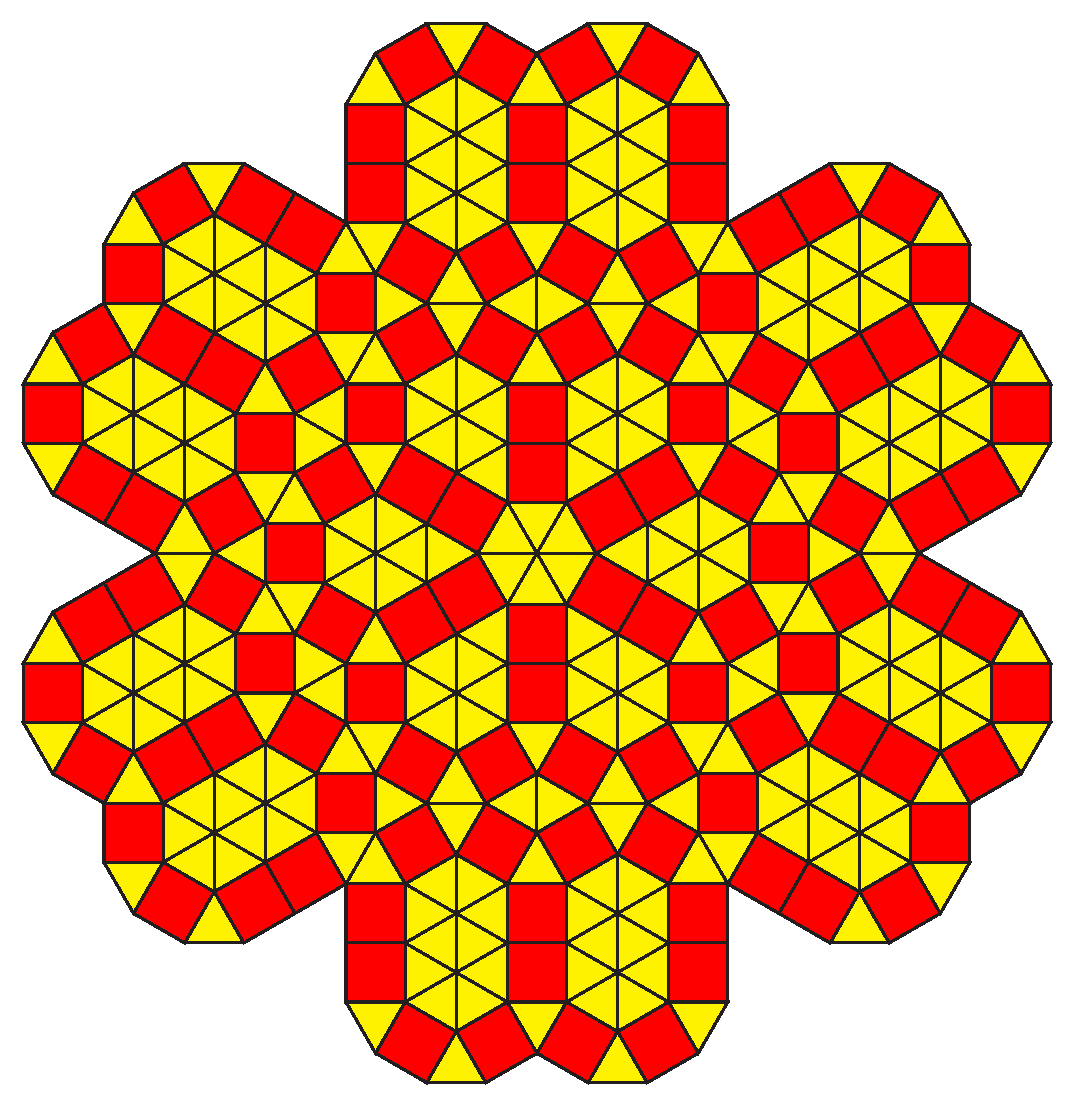
\includegraphics[width=0.8\linewidth]{rosaceastrica.eps}
\end{center}
\vfill

\strut



\endinput
    %chapfstd
\chapter{Les formes libres}\label{chapflib}

\section{Introduction}

Comme le menu A, les menus B et C proposent des \textbf{\textit{objets}} et des
\textbf{\textit{fonctionnalit�s}}.\index{Menu!B}\index{Menu!C}

Les objets des menus B et C sont des formes dites \og libres\fg\index{Forme!libre}.
Elles sont rassembl�es en familles d�finies par leur nombre de c�t�s,
la r�gularit�\ldots\  � la diff�rence des formes standard, (mis � part le point) elles
n'apparaissent plus d'un simple clic � l'�cran.
L'utilisateur les construit lui-m�me  en fixant plusieurs sommets, un � la fois.

Les menus B et C sont tr�s proches. En ce qui concerne les formes g�om�triques accessibles, le menu C se
distingue du  menu B par le fait qu'il propose des objets \og illimit�s\fg: droites\index{Droite},
demi-droites\index{Demi-droite}, secteurs\index{Secteur} et bandes\index{Bande}. Il propose �galement un autre type d'objet absent du menu B:
des secteurs de disque\index{Secteur!de disque}.

Les formes libres sont construites par le positionnement de leurs sommets � l'aide de clics de la souris. Par un clic de
souris, nous pouvons construire trois  esp�ces de points (du point de vue informatique, les points n'existent pas tant
qu'ils n'ont pas �t� construits):

\begin{list}{\textbullet}{\itemsep=1mm} \item Les
\hyperdef{chapflib}{PointLibre}{points libres}\index{Point!libre}: un point de ce
type poss�de deux degr�s de libert�. Les seules contraintes auxquelles il doit
ob�ir sont celles qui r�sultent de son appartenance �ventuelle en tant que sommet �
une forme g�om�trique particuli�re (triangle rectangle par exemple). Un point
libre est obtenu par un clic en un emplacement libre de l'�cran.

\item Les \hyperdef{chapflib}{PointLie}{points
li�s}\index{Point!li�}\index{Point!sur} au bord d'une forme g�om�trique : un point
de ce type n'a  qu'un degr� de libert�. Il ne peut se d�placer que sur le bord de
la forme sur laquelle il a �t� plac�. (Voir aussi
\hyperlink{chapcontext.Limiter}{\texttt{Limiter}}.) C'est pourquoi nous utiliserons
souvent l'expression \og point sur\fg. Un \og point sur\fg\ est obtenu par un clic
sur le bord d'une forme pr�existante.

\danger\hfill\fbox{\begin{minipage}{0.89\linewidth}
\begin{minipage}[b]{0.75\linewidth}\label{chapflibptsurdeuxf} Il peut se faire qu'un point soit plac� sur  un
segment commun � deux formes. Dans ce cas le logiciel consid�re que le point en question est un  point \og
sur\fg\ celle des deux formes qui est � l'avant-plan par rapport � l'autre. Par d�faut, c'est celle qui a �t�
construite en dernier lieu. \end{minipage}\hfill \begin{minipage}[b]{0.2\linewidth}
\includegraphics[width=\linewidth]{ptsurdeuxformes.eps} \leg{} \end{minipage}  L'utilisateur peut modifier la
position d'une forme par rapport � l'autre, via les proc�dures
\hyperlink{chapoutils.Plans}{\texttt{Avant-plan}}\index{Avant-plan} et
\hyperlink{chapoutils.Plans}{\texttt{Arri�re-plan}}.\index{Arri�re-plan}    Sur la figure ci-dessus, le
triangle $bcd$ a �t� construit apr�s le triangle $abd$. Le point $p$ a �t� plac� ensuite. Il est donc \og
sur\fg\ le triangle $bcd$ et mobile sur le bord de ce triangle.\end{minipage}}


\item Un \hyperdef{chapflib}{PointInter}{point d'intersection}\index{Point!d'intersection} est
comme son nom l'indique plac� � l'intersection de deux objets. Il n'a aucun degr� de libert�: il ne
pourra changer de place que si l'une des deux formes qui le d�terminent est modifi�e. \end{list}

Aux chapitres \ref{chapoper} et \ref{chaptsf}, nous rencontrerons une quatri�me esp�ce de
points: des \hyperdef{chapflib}{PointCsted}{points construits}\index{Point!construit}
� partir d'une forme g�om�trique pr�existante. Par exemple, le centre
d'un polygone d�pend enti�rement de ce polygone, sa
construction n�cessite l'emploi d'une \textit{Op�ration}\index{Operation@Op�ration}.

\section{Des formes orient�es}

Les points mis � part, toutes les formes libres sont des formes
\textit{orient�es}.\index{Orientation}\index{Forme!orient�e} Leur orientation
est d�termin�e par l'ordre de construction des sommets. Les segments $[a,b]$ et
$[b,a]$ ne peuvent �tre consid�r�s comme identiques, pas plus que  les triangles
$abc$ et $cba$. Par contre $cab$ et $bca$ ont les m�mes propri�t�s que $abc$ et
ne doivent donc pas �tre distingu�s.

 On voit appara�tre l� une diff�rence entre la g�om�trie euclidienne usuelle et la
g�om�trie dynamique. Dans la suite, nous aurons l'occasion de revenir sur cette
question, notamment lorsqu'au chapitre \ref{chapoutils}, nous parlerons des
\hyperlink{chapoutils.Mesure}{\textit{mesures}}.



\section{Formes Libres}

� l'ouverture d'\AG\ avec un des menus B ou  C,  les familles de formes libres apparaissent dans un des pav�s de la bo�te �
outils. Ce pav�, constitu� des \textit{Formes Libres}, comprend sept ic�nes activables par un clic de souris. �
l'activation d'une d'elles, l'ic�ne est encadr�e en rouge et une fen�tre compos�e de 2 � 10 boutons poussoirs appara�t
alors � l'�cran pour choisir la forme � construire (sauf si on a choisi l'ic�ne repr�sentant un point:
seul le cadre rouge est dessin�).

\fbox{\begin{minipage}{\linewidth}

\Prat

\begin{minipage}[c]{0.15\linewidth}
\includegraphics[width=\linewidth]{FormesLibres.jpg}
\leg{}
\end{minipage}
\hfill
\begin{minipage}[c]{0.82\linewidth}\parskip 2mm
\begin{list}{\textbullet}{\itemsep=1mm\leftmargin=3mm}
\item La construction  d'une forme est initialis�e par
un premier clic sur le bouton poussoir portant le nom de la forme souhait�e.

\item Chaque clic de la souris dans la fen�tre de travail fixe alors un sommet de la forme souhait�e,
le logiciel veillant au respect des contraintes g�om�triques.


\item Il est ainsi possible de fixer � l'�cran aussi bien des points  libres, que des points li�s � un
objet ou encore des points � l'intersection de deux objets.

\begin{itemize} \item Pour lier un point � un objet d�j� dessin�, approcher le point
mobile (situ� � l'extr�mit� du curseur de la souris) de l'objet jusqu'� ce que, gr�ce au
 magn�tisme\index{Magnetisme@Magn�tisme}, la couleur de celui-ci  passe au magenta. Le
clic de la souris place alors  le point sur l'objet.\index{Point!sur} Le point est
devenu un \og point sur\fg.
\end{itemize}
\end{list}
\end{minipage}

\begin{itemize}
\item Pour placer un  point � l'intersection de deux formes, proc�der de m�me en approchant le point mobile de
l'intersection vis�e. Le clic fixe le point � cette intersection\index{Intersection} pour autant que les  bords des formes
aient tous deux vir� au magenta.\index{Point!d'intersection}
\end{itemize}
\end{minipage}}

\danger\hfill\fbox{\begin{minipage}[t]{0.89\linewidth} Comme lors de la construction d'une forme standard, il peut
arriver que l'utilisateur r�alise involontairement un \og \hyperlink{chapfstd.doubleclic}{double clic}\fg. Relisez
le paragraphe consacr� � cette question � la page \pageref{doubleclic}.\end{minipage}}

Pour pouvoir placer un point � l'\hyperdef{chaplib}{inter}{intersection} de deux formes, il faut que point d'intersection puisse �tre identifi� de fa�on univoque.
Ce n'est pas toujours le cas. En particulier, on peut souhaiter placer un point sur un segment qui apparaisse commun � deux formes, comme dans la situation de
la figure \ref{chapflib.ptinter}.

\strut\hfill
\begin{minipage}[b]{0.25\linewidth}
\includegraphics[width=\linewidth]{Deuxtri.eps}
\leg{\label{chapflib.ptinter}}
\end{minipage}
\hfill
\begin{minipage}[b]{0.3\linewidth}
\includegraphics[width=\linewidth]{DeuxtriBis.jpg}
\leg{\label{chapflib.ptinterbis}}
\end{minipage}
\hfill\strut

� l'emplacement du c�t� commun aux deux triangles se trouvent en r�alit� deux segments superpos�s. L'intersection de ces deux segments n'�tant pas r�duite � un point,
le logiciel ne peut placer un nouveau point que sur l'un d'entre eux. Il choisit le triangle situ� � l'avant-plan, le colore en magenta et propose ce choix �
l'utilisateur (figure \ref{chapflib.ptinterbis}).
Si c'est l'autre triangle que l'on veut choisir,  il convient de le mettre au pr�alable � l'avant-plan.


\subsection{La famille du point}

Cette famille  ne contient que le \hyperdef{chapflib}{Point}{point.}\index{Point} Un seul clic suffit
� construire un point, de l'une des trois esp�ces mentionn�es plus haut.

\subsection{La famille des segments}
\index{Segment}\label{Segment}

Le menu \textit{B}\index{Menu!B} ne permet de dessiner que des segments, �ventuellement parall�les ou
perpendiculaires �  un autre objet.
\index{Segment!perpendiculaire}\index{Segment!parall�le}

Le menu \textit{C}\index{Menu!C} permet, en plus, de dessiner des droites, �ventuellement parall�les
ou perpendiculaires � un autre objet, des demi-droites, des secteurs et des
bandes.\index{Droite}\index{Droite!perpendiculaire}\index{Droite!parall�le}\index{Secteur}\index{Bande}

Si un segment ou une droite est parall�le ou
perpendiculaire � \textit{un autre objet}, celui-ci peut �tre un segment, une
droite, une demi-droite, un c�t� de polygone, un bord de bande ou un bord de
secteur.\index{Bande}\index{Secteur}\index{Polygone}\index{Demi-droite}

\begin{list}{\textbullet}{\itemsep=0mm}  \item Pour tracer un
\hyperdef{chapflib}{Segment}{\textit{segment},} fixer les extr�mit�s en deux clics
de souris. L'ordre dans lequel les extr�mit�s d'un segment ont �t� fix�s
d�termine l'orientation de ce segment\index{Orientation!d'un segment}. \item
Pour tracer un \textit{segment parall�le} � un autre objet, s�lectionner cet objet
et apr�s avoir rel�ch� le bouton de la souris, d�placer celle-ci jusqu'�
l'emplacement choisi pour l'origine du nouveau segment, cliquer et tirer � la
souris jusqu'� l'extr�mit� souhait�e. \item Pour tracer un \textit{segment
perpendiculaire} � un autre objet, la proc�dure est
identique.\index{Segment!parall�le}\index{Segment!perpendiculaire}

\item Pour tracer une \textit{droite}, fixer deux points en deux clics de souris.
\item Pour tracer une \textit{droite parall�le} � un autre  objet,  s�lectionner cet objet et apr�s avoir rel�ch� le bouton de la
souris, d�placer celle-ci jusqu'� l'emplacement choisi pour y fixer un point de
la droite parall�le. \item Pour tracer une \textit{droite perpendiculaire} � une
autre  objet, la proc�dure est identique.
\index{Droite!parall�le}\index{Droite!perpendiculaire}

 \item Pour tracer une \textit{demi-droite}, en deux clics de souris, fixer son
origine puis un autre point. \item Pour tracer une \textit{bande}, trois clics sont n�cessaires: les deux premiers
d�terminent un des deux bords de la bande, le troisi�me d�termine l'autre bord.  \item Pour tracer un \textit{secteur},
� nouveau trois clics sont n�cessaires. Dans l'ordre: le sommet du secteur, un point du premier c�t�, un point du second.
\index{Droite}\index{Demi-droite}\index{Bande}\index{Secteur}
\end{list}



\subsection{La famille des triangles}

\index{Triangle}

\fbox{\begin{minipage}[b]{0.99\linewidth}
\begin{minipage}[b][9cm][t]{0.25\linewidth}
\includegraphics[width=\linewidth]{triangles.bmp}
\begin{minipage}[b]{1.25cm}
\leg{}
\end{minipage}
\end{minipage}\hfill
\begin{minipage}[b][9cm][t]{0.70\linewidth}
\begin{minipage}[b]{0.10\linewidth}
\includegraphics[width =\linewidth]{triqcq.eps} \leg{} \end{minipage} \hfill
\begin{minipage}[b]{0.80\linewidth}Pour tracer un \hyperdef{chapflib}{Triangle}{\textit{triangle
quelconque}}: en trois clics, fixer les sommets. \end{minipage} \medskip \index{Triangle!quelconque}

\begin{minipage}[b]{0.10\linewidth}
\includegraphics[width =\linewidth]{triiso.eps}
\leg{}
\end{minipage}\hfill
\begin{minipage}[b]{0.80\linewidth}Pour tracer un \textit{triangle isoc�le}, les deux premiers clics
fixent \og la\fg\ base du triangle et le
troisi�me clic fixe le troisi�me sommet. \end{minipage} \index{Triangle!isoc�le}\medskip

\hskip-0.25\linewidth
\begin{minipage}[b]{0.10\linewidth}
\includegraphics[width =\linewidth]{triequi.eps}
\leg{}
\end{minipage}\hfill
\begin{minipage}[b]{1.05\linewidth}Pour tracer
un \textit{triangle �quilat�ral}, deux clics suffisent � fixer deux sommets, le logiciel fixe le
troisi�me en orientant le triangle dans le sens trigonom�trique positif. \end{minipage}
\index{Triangle!�quilat�ral}
\medskip

\hskip-0.25\linewidth
\begin{minipage}[b]{0.10\linewidth}
\includegraphics[width =\linewidth]{trirect.eps}
\leg{}
\end{minipage}\hfill
\begin{minipage}[b]{1.05\linewidth}Pour tracer
un \textit{triangle rectangle}, trois clics fixent successivement un sommet d'angle aigu, le
sommet de l'angle droit, le sommet du deuxi�me angle aigu. \end{minipage}\index{Triangle!rectangle}
\medskip

\hskip-0.25\linewidth
\begin{minipage}[b]{0.10\linewidth}
\includegraphics[width =\linewidth]{trirectiso.eps}
\leg{}
\end{minipage}\hfill
\begin{minipage}[b]{1.05\linewidth}Pour tracer
un \textit{triangle rectangle isoc�le}, deux clics de souris suffisent � fixer les sommets
des angles aigus, le logiciel fixant le troisi�me sommet, �galement en respectant le sens
trigonom�trique. \end{minipage}\index{Triangle!rectangle  isoc�le}
\end{minipage}
\end{minipage}}


\subsection{La famille des quadrilat�res}

\fbox{\begin{minipage}[b]{0.99\linewidth}\parskip1mm
\begin{minipage}[t][5.5cm][t]{0.25\linewidth}
\leavevmode\space\\
\includegraphics[width=\linewidth]{quadr.bmp}
\leg{}
\end{minipage}\hfill
\begin{minipage}[t]{0.70\linewidth}
\leavevmode\space\\
\begin{minipage}[c]{0.10\linewidth}
\includegraphics[height = 2\baselineskip]{quadrqcq.eps} \leg{}
\end{minipage} \hfill
\begin{minipage}[c]{0.80\linewidth}
Pour tracer un \hyperdef{chapflib}{Quadrilatere}{\textit{quadrilat�re
quelconque}}: en quatre clics, fixer les sommets.
\end{minipage}\medskip \index{Quadrilat�re!quelconque}

\begin{minipage}[c]{0.10\linewidth} \includegraphics[height =
2\baselineskip]{trap.eps} \leg{} \end{minipage}\hfill
\begin{minipage}[c]{0.80\linewidth}Pour tracer un
\hyperdef{chapflib}{Trapeze}{\textit{trap�ze}}, les deux premiers clics fixent une
des bases, les deux suivants l'autre base. \end{minipage} \index{Trap�ze}\medskip

\begin{minipage}[c]{0.10\linewidth} \includegraphics[height = 2\baselineskip]
{traprect.eps} \leg{} \end{minipage}\hfill
\begin{minipage}[c]{0.80\linewidth}Pour tracer un \textit{trap�ze rectangle},
trois clics suffisent. Le premier fixe un sommet d'angle droit et les deux
suivants les sommets des angles non droits. \end{minipage}
\index{Trap�ze!rectangle}


\begin{minipage}[c]{0.10\linewidth} \includegraphics[height =
2\baselineskip]{trapiso.eps} \leg{} \end{minipage}\hfill
\begin{minipage}[c]{0.80\linewidth}Pour tracer un \textit{trap�ze isoc�le}, trois
clics suffisent �galement. Les deux premiers fixent une base, le troisi�me un
sommet de l'autre base. \end{minipage} \index{Trap�ze!isoc�le}

\hskip-0.35\linewidth
\begin{minipage}[c]{0.10\linewidth} \includegraphics[height
= 2\baselineskip]{parall.eps} \leg{} \end{minipage}\hfill
\begin{minipage}[c]{1.05\linewidth}Pour tracer un \textit{parall�logramme}, trois
clics d�terminent deux c�t�s adjacents, ce qui permet au logiciel de terminer la
construction.\end{minipage}\index{Parall�logramme}

\hskip-0.35\linewidth \begin{minipage}[c]{0.10\linewidth} \includegraphics[height =
2\baselineskip]{rect.eps} \leg{} \end{minipage}\hfill
\begin{minipage}[c]{1.05\linewidth}Pour tracer un \textit{rectangle}, ou un \textit{losange} la proc�dure
est la m�me que pour un parall�logramme. Le logiciel veille au respect des contraintes d'angle ou de longueur.
\end{minipage}\index{Rectangle}\index{Losange}


%\hskip-0.35\linewidth \begin{minipage}[c]{0.10\linewidth}
%\includegraphics[height = 2\baselineskip]{losange.eps}
%\leg{} \end{minipage}\hfill
%\begin{minipage}[c]{1.05\linewidth}Pour tracer un \textit{losange}, la proc�dure
%est encore identique.
%\end{minipage}\index{Losange}


\hskip-0.35\linewidth
\begin{minipage}[c]{0.10\linewidth}
\centerline{\includegraphics[height = 2\baselineskip]{carre.eps}} \leg{}
\end{minipage}\hfill \begin{minipage}[c]{1.05\linewidth}Pour tracer un carr�,
deux clics d�terminent un c�t�, le logiciel termine le travail en respectant le
sens trigonom�trique de parcours.
\end{minipage}


\end{minipage}
\end{minipage}\index{Carre@Carr�}}




\subsection{La famille des polygones r�guliers}
\index{Polygone!r�gulier}\index{Triangle!�quilat�ral}\index{Carre@Carr�}\index{Pentagone}\index{Hexagone}\index{Heptagone}
\index{Octogone}\index{Enneagone@Enn�agone}\index{Decagone@D�cagone}\index{Hend�cagone}\index{Dod�cagone}
\fbox{\begin{minipage}[b]{0.99\linewidth}
\begin{minipage}[b]{0.25\linewidth}
\includegraphics[width=\linewidth]{polygreg.bmp}
\leg{}
\end{minipage}
\begin{minipage}[b]{0.73\linewidth} Pour tracer un \hyperdef{chapflib}{Polreg}{\textit{polygone r�gulier}}
de trois � douze c�t�s, deux clics fixent un c�t�. Le logiciel termine le trac� en respectant le sens
trigonom�trique de parcours.\vspace{1cm} \begin{center}
\includegraphics[width=0.6\linewidth]{polregs.eps} \leg{} \end{center} \end{minipage}
\end{minipage}}

\subsection{La famille du cercle}
\label{Constructioncercle}
\fbox{\begin{minipage}[b]{0.99\linewidth}
\begin{minipage}[c]{0.25\linewidth}
\includegraphics[width=\linewidth]{cercles.bmp} \leg{}
\end{minipage}
\begin{minipage}[c]{0.73\linewidth}
\begin{minipage}[c]{0.15\linewidth}
\includegraphics[width =\linewidth]{cercle.eps} \leg{}
\end{minipage} \hfill
\begin{minipage}[c]{0.85\linewidth}Pour tracer un
\hyperdef{chapflib}{Cercle}{\textit{cercle}}, deux clics suffisent: le premier
fixe le centre, le second fixe un point du cercle.
\end{minipage}\index{Cercle}
\end{minipage}\\
\begin{minipage}[c]{0.15\linewidth} \includegraphics[width =0.77\linewidth]{arc.eps}
\leg{} \end{minipage} \hfill \begin{minipage}[c]{0.83\linewidth}Pour tracer un
\textit{arc de cercle}, trois clics sont n�cessaires. Le premier fixe  le centre
du cercle, le second l'origine de l'arc, le troisi�me l'extr�mit�. Ces arcs de
cercle sont orient�s. \end{minipage}\index{Arc}\\

\begin{minipage}[c]{0.15\linewidth} \includegraphics[width =0.77\linewidth]{SectDisk.eps}
\leg{} \end{minipage} \hfill \begin{minipage}[c]{0.83\linewidth}Depuis la version 2.5.0, le menu C
permet �galement de dessiner un \textit{secteur de disque}. La construction est semblable � celle d'un arc de cercle.
\end{minipage}\index{Secteur!de disque}
\end{minipage}}



Lors de la construction, tout cercle est orient�\index{Orientation!d'un cercle} dans
le sens trigonom�trique. � chaque \textit{retournement}\index{Retournement} qui
lui est appliqu�, l'orientation est invers�e.

L'orientation d'un arc de cercle\index{Orientation!d'un arc de cercle} et celle d'un secteur de disque\index{Orientation!d'un secteur de disque}
sont toujours de l'origine de l'arc vers son extr�mit�.
 

\subsection{La famille des polygones quelconques}

\index{Polygone!quelconque}
\index{Triangle}\index{Quadrilat�re}\index{Pentagone}\index{Hexagone}\index{Heptagone}
\index{Octogone}\index{Enneagone@Enn�agone}\index{Decagone@D�cagone}\index{Hend�cagone}\index{Dod�cagone}

\fbox{\begin{minipage}[b]{0.99\linewidth}
\begin{minipage}[b]{0.25\linewidth}
\includegraphics[width=\linewidth]{polygqcq.bmp}
\leg{}
\end{minipage}
\hfill
\begin{minipage}[b]{0.66\linewidth}
Pour tracer un \hyperdef{chapflib}{Polyqcq}{\textit{polygone
quelconque}} de trois � douze c�t�s, on fixe les sommets un � la fois en autant de clics qu'il y a
de sommets � fixer. Ces polygones peuvent ne pas �tre convexes.\medskip

\centering
\includegraphics[width=0.5\linewidth]{polygs.eps}
\leg{}
\vspace{1cm}
\end{minipage}
 \end{minipage}}

\section{Abandonner une construction}

\hyperdef{chapflib}{Abandonner}{L'utilisateur} peut toujours abandonner la construction d'une forme
libre avant que celle-ci soit achev�e. Il actionnera dans ce but le bouton
\texttt{Annuler}\index{Annuler}. Pour plus d'informations � propos de cette fonctionnalit�, voir la
section \hyperlink{chapmedit.Annuler}{\texttt{�dition/Annuler}}.

\section{Une remarque}

Un logiciel tel que \AG\ met en \oe uvre des contraintes de deux types: g�om�triques d'une part,
informatiques d'autre part.  Lorsqu'on r�alise une figure, il n'y a pas int�r�t � superposer des
contraintes alors que certaines seraient automatiquement r�alis�es. Prenons un exemple en
r�alisant la figure du th�or�me de Varignon: \textit{Le quadrilat�re $mnpq$ obtenu en
joignant les milieux des c�t�s d'un quadrilat�re $abcd$ est un parall�logramme.}

\begin{center}
\begin{minipage}[b]{0.3\linewidth}
\includegraphics[width=\linewidth]{varignon.eps}\medskip

\leg{}
\end{minipage}
\end{center}

Pour r�aliser cette figure, l'utilisateur va
dessiner d'abord le
quadrilat�re $abcd$ en utilisant le bouton \texttt{Quadrilat�res/Quadrilat�re}
du pav� des \textit{Formes Libres};

 Ensuite, l'op�ration
\hyperlink{chapoper.Diviser}{\texttt{Diviser}} du chapitre \ref{chapoper}
lui permet de construire les milieux $m$, $n$, $p$, $q$ des c�t�s de $abcd$.

Il lui reste � joindre les points $m$, $n$, $p$, $q$. S'il ignore que ces points
sont sommets d'un parall�logramme, l'utilisateur va normalement r�utiliser le
bouton \texttt{Quadrilat�res/Quadrilat�re}. Il constatera alors que ce
quadrilat�re est un parall�logramme: c'est la g�om�trie qui l'impose.

 Mais si l'utilisateur sait que $mnpq$ est un parall�logramme, il pourrait �tre
tent� d'utiliser le bouton \texttt{Quadrilat�res/Parall�logramme}. Bien s�r, il
obtiendrait la m�me figure, du moins en apparence. En effet, pour construire ce
parall�logramme, il suffit d'indiquer au logiciel trois sommets, par exemple $m$,
$n$, $p$. \AG\ compl�te alors le parall�logramme en calculant la position du
quatri�me sommet et en le cr�ant, sans tenir compte de l'existence du point $q$.
Ainsi, d'une part on a cr�� une contrainte informatique dont on aurait pu se
passer, mais surtout, en $q$ se trouveront en r�alit� deux points: l'un est le
milieu du c�t� $[d,a]$ du quadrilat�re $abcd$, l'autre est le quatri�me sommet du
parall�logramme construit par le  logiciel � partir des trois points $m$, $n$ et
$p$. Ainsi les quatre sommets du parall�logramme n'ont pas le m�me statut. Si la
figure se limite au quadrilat�re et au parall�logramme, il n'en r�sulte aucune
cons�quence f�cheuse. Mais cela pourrait entra�ner une confusion et des
inconv�nients difficiles � comprendre si la complexit� de la figure augmente
et qu'on  r�utilise le point $q$, sans �tre conscient de son d�doublement.

Ces inconv�nients sont �vit�s en ne superposant pas une contrainte informatique � la contrainte g�om�trique
existante.




\endinput

%%%%%%%%%%%%%%%%%%%%%%%%%%%%%%%%%%%%%%%%%%%%%%%%%%%%%%%%%%%%%%%%%%%%%%%

   %chapflib
\chapter{Fichier, Fen�tres et �dition}\label{chapmedit}

\section{Introduction}

Les trois premiers menus d�roulants sont � peu pr�s ind�pendants du choix effectu� par l'utilisateur
entre \textit{Menu A, B} ou \textit{C}. De plus, ils pr�sentent des proc�dures courantes dans les
programmes informatiques, ce qui nous permettra de ne pas nous y attarder trop.


\section{Fichier}

\begin{center}
\includegraphics[width=0.25\linewidth]{Menu_Fichier.bmp}
\leg{}
\end{center}



\subsection{Fichier/Nouveau}

� l'ouverture du logiciel, une feuille de travail est ouverte  automatiquement.
L'option \texttt{Nouveau}\index{Fichier!Nouveau} permet de cr�er des feuilles de
travail suppl�mentaires. Plusieurs
feuilles de travail peuvent ainsi �tre ouvertes successivement\ldots\
pour autant que l'ordinateur poss�de suffisamment de m�moire libre. Gr�ce au
menu \hyperdef{chapmedit}{Fenetres}{\texttt{Fen�tres}},  on peut passer de l'une
� l'autre (nous y reviendrons plus loin). La  barre de titre de chaque fen�tre
fournit les informations suivantes: le nom de l'utilisateur, le nom du fichier
de sauvegarde (s'il en existe d�j� un), l'identification de l'op�ration active,
et enfin le mot \og Figure\fg\ suivi du num�ro de la fen�tre. Dans ce contexte,
le mot \og Figure\fg\ d�signe l'ensemble des formes g�om�triques qui ont �t�
dessin�es dans la fen�tre.  De plus, si la figure a �t� modifi�e depuis la
derni�re sauvegarde, une �toile appara�t � la fin de cette ligne.

\subsection{Fichier/Ouvrir}

\hyperdef{chapmedit}{Ouvrir}{\texttt{Ouvrir}}\index{Fichier!Ouvrir} ouvre un fichier d'extension
\texttt{.fag}\index{.fag@\texttt{.fag}} d�j� enregistr� sur un disque dur ou sur un support amovible (cl�
USB, c�d�rom, disquette\dots) et l'affiche dans une  nouvelle feuille de travail (sauf si la feuille en
cours est toujours vierge).

\subsection{Fichier/Fermer}

\hyperdef{chapmedit}{Fermer}{\texttt{Fermer}}\index{Fichier!Fermer}  cl�t  la feuille de travail en
cours. Si celle-ci n'a pas �t� modifi�e depuis la derni�re sauvegarde, elle se ferme sans devoir �tre
enregistr�e. Par contre, si un changement est intervenu, une confirmation est demand�e � l'utilisateur
qui peut encore sauvegarder son travail.\medskip

\centerline{\begin{minipage}[b]{0.4\linewidth}
\includegraphics[width=\linewidth]{Fermer.bmp}
\leg{}
\end{minipage}}

\subsection{Fichier/Standardiser}\index{Standardiser}

L'op�ration \texttt{Standardiser} permet de cr�er de nouvelles familles de formes standard. Elle a �t� d�crite � la section \ref{chapfstd.stdiser}.


\subsection{Fichier/Sauvegarder}

\hyperdef{chapmedit}{Sauvegarder}{\texttt{Sauvegarder}}\index{Fichier!Sauvegarder} enregistre le contenu
de la feuille de travail dans  un fichier d'extension \texttt{.fag}\index{.fag@\texttt{.fag}}.
Lors du premier enregistrement d'un fichier, cliquer sur l'option \texttt{Sauvegarder} revient
� cliquer sur l'option \texttt{Sauvegarder sous}. Lorsqu'un fichier est enregistr�, son nom appara�t
dans la barre de titre de la fen�tre � la suite du nom de l'utilisateur. Ensuite, tout clic sur \texttt{Sauvegarder}
enregistre la figure dans le m�me dossier et sous le m�me nom.

Les fichiers de sauvegarde, d'extension \texttt{.fag} sont �crits en langage
\texttt{xml}, comme les fichiers d'extension \texttt{.std} dont il a �t� question
au chapitre \ref{chapfstd}. Ils peuvent �tre lus avec n'importe quel �diteur de
texte, mais, sous \texttt{Windows},  nous recommandons le logiciel gratuit \texttt{xmlnotepad} qui respecte
la structure du texte en mettant les balises en �vidence.

\textbf{Remarque}
 
 En plus des informations relatives aux diff�rents objets g�om�triques, le fichier
de sauvegarde  contient �galement les informations relatives � la configuration de
l'application ainsi que la langue de travail, au moment de la sauvegarde.
L'environnement de travail est ainsi restaur� lors de la r�ouverture du fichier.


\subsection{Fichier/Sauvegarder sous}

 \hyperdef{chapmedit}{Sauvegardersous}{\texttt{Sauvegarder
sous}}\index{Fichier!Sauvegarder sous} enregistre le fichier � un endroit �
sp�cifier  � partir d'une fen�tre de dialogue. Le nom du
fichier appara�t ensuite dans la barre de titre de la fen�tre � c�t� des mentions
relatives � l'utilisateur.
On utilise aussi cette option si on souhaite enregistrer un fichier sous un nom
diff�rent de son nom actuel ou dans un dossier diff�rent.

Il est d�conseill� d'ins�rer des caract�res
accentu�s dans un titre de fichier: des probl�mes pourraient appara�tre par
exemple si un fichier r�alis� sous \texttt{Windows} �tait relu par un
\texttt{Macintosh}.



\subsection{Fichier/Exporter en Postscript}
 
\hyperdef{chapmedit}{ExportPS}{\texttt{Exporter en Postscript}}\index{Fichier!Exporter en
Postscript} n'est accessible  qu'aux enseignants. Cette option permet d'exporter tout ou
partie de la figure dessin�e dans la feuille de travail dans un fichier de format
\texttt{.eps}\index{.eps@\texttt{.eps}}. Par d�faut, l'int�gralit� de la figure est
export�e. On peut n'exporter que certaines des formes g�om�triques en les s�lectionnant
avant de lancer l'op�ration d'exportation. Pour la proc�dure de s�lection, voir la
section \hyperlink{chapmedit.Selectionner}{\sffamily\bfseries �dition/S�lectionner}.

Les fichiers d'extension \texttt{.eps} sont r�dig�s en langage \texttt{postscript}. Ils peuvent  �tre
�dit�s  gr�ce � un �diteur de texte classique et visualis�s gr�ce au
logiciel \texttt{GsView} par exemple. Ils peuvent �galement �tre modifi�s gr�ce � un logiciel du type
\texttt{Illustrator}.



\subsection{Fichier/Exporter en fichier bitmap}

\hyperdef{chapmedit}{ExportBMP}{\texttt{Exporter en fichier bitmap}}\index{Fichier!Exporter en fichier bitmap}
permet de recopier une partie de l'�cran dans un fichier image. La proc�dure consiste � dessiner � la souris
un rectangle sur l'�cran (cliquer � l'emplacement du coin sup�rieur gauche, puis tirer le curseur jusqu'�
l'emplacement souhait� pour le coin inf�rieur droit). L'image � sauvegarder est �videmment constitu�e de
l'int�rieur du rectangle qui a �t� dessin�. Quand on rel�che le bouton de la souris, un peu de temps s'�coule,
puis appara�t une boite de dialogue o� l'on peut indiquer le nom du fichier � cr�er.\medskip

\centerline{\begin{minipage}[b]{0.7\linewidth}
\includegraphics[width=\linewidth]{ExportBMP.bmp}
\leg{}
\end{minipage}}

La petite fen�tre dans la partie inf�rieure gauche de cette bo�te de dialogue cache un menu d�roulant
dans laquelle l'utilisateur peut choisir le type d'image de son choix (\texttt{.jpg},
\texttt{.bmp}\ldots)\index{.jpg@\texttt{.jpg}}, � condition de travailler sous \texttt{Windows}
ou sur un \texttt{Macintosh} et que le programme \texttt{QuickTime} soit pr�sent sur son ordinateur.
Dans le cas contraire, le seul format disponible sous \texttt{Windows} est le format
\texttt{.bmp}\index{.bmp@\texttt{.bmp}}, tandis que sur un \texttt{Macintosh} c'est le format \texttt{.pict}\index{.pict@\texttt{.pict}}.
Sous \texttt{Linux}, seul le format
\texttt{.bmp} est disponible. Ces contraintes r�sultent du langage de programmation utilis�.

 


\subsection{Fichier/Param�tres d'impression}

\hyperdef{chapmedit}{ParamImp}{\texttt{Param�tres d'impression}}\index{Fichier!Param�tres d'impression}
affiche une fen�tre de dialogue dans laquelle sont propos�s le choix du papier (taille et source), de
l'orientation de l'impression (portrait ou paysage) et des marges en millim�tres (gauche, droite, haut
et bas).

\subsection{Fichier/Imprimer}

\hyperdef{chapmedit}{Imprimer}{\texttt{Imprimer}}\index{Fichier!Imprimer} imprime la figure pr�sente �
l'�cran. � l'impression, la fen�tre de travail repr�sente environ la moiti� d'une page format A4 en
orientation \textit {portrait}. Par d�faut, toutes les formes pr�sentes � l'�cran sont imprim�es. On
peut n'imprimer que certaines des formes g�om�triques en les s�lectionnant avant de lancer
l'impression. Pour la proc�dure de s�lection, voir la section
\hyperlink{chapmedit.Selectionner}{\sffamily\bfseries �dition/S�lectionner}.



\subsection{Fichier/Quitter}


\hyperdef{chapmedit}{Quit}{\texttt{Quitter}}\index{Fichier!Quitter} ferme l'application. Le logiciel
propose au pr�alable d'enregistrer la ou les figures r�alis�es qui auraient �t� modifi�es depuis la
derni�re sauvegarde.

\danger\hfill\fbox{\begin{minipage}{0.89\linewidth} Comme tout programme informatique, et malgr� les
efforts de ses concepteurs, \AG\ peut contenir des \og bugs\fg\index{Bug}. Lorsqu'un d'entre eux se
manifeste, le logiciel doit afficher la bo�te de dialogue suivante, pour autant que l'ordinateur soit
connect� sur Internet:\medskip

\centerline{\begin{minipage}[b]{0.7\linewidth}
\includegraphics[width=\linewidth]{Bug.bmp}
\leg{}
\end{minipage}}

Si l'utilisateur accepte de signaler l'erreur, l'ordinateur envoie au serveur du
\textsc{crem} un message indiquant la nature de l'erreur, ainsi qu'une copie de
la figure courante, ceci afin d'aider les programmeurs � d�tecter et corriger le
probl�me apparu.  Si l'ordinateur n'est pas connect� sur Internet, seul le
message d'excuses appara�t. Dans tous les cas, l'ordinateur laisse ouverte  la feuille de
travail sur laquelle l'erreur s'est produite, g�n�ralement dans l'�tat pr�c�dant celle-ci. L'utilisateur
peut essayer de poursuivre son travail, en �vitant de r�p�ter les op�rations ayant provoqu� l'erreur. Il lui est d�s lors conseill� de sauvegarder
son travail r�guli�rement. Les �ventuelles autres feuilles de
travail restent accessibles et pleinement fonctionnelles. \end{minipage}}

\section{Fen�tres}


\begin{minipage}[b]{0.15\linewidth}
\includegraphics[width=\linewidth]{Menu_Fenetres.bmp}
\leg{}
\end{minipage}\hfill
\begin{minipage}[b]{0.8\linewidth}
Ce menu,   permet d'acc�der facilement aux feuilles de travail existantes.
Chaque  nouvelle feuille de travail  se superpose aux pr�c�dentes et le compteur de fen�tres est incr�ment�.

Lorsqu'on d�roule le menu, la figure active est coch�e. On en affiche une autre  en cochant l'item
de menu correspondant.
\end{minipage}


\section{�dition}

\begin{minipage}[b]{0.25\linewidth} \includegraphics[width=\linewidth]{Menu_Edition.bmp}
\leg{} \end{minipage}\hfill
\begin{minipage}[b]{0.7\linewidth} Certaines des op�rations
pr�sentes dans ce menu se retrouvent dans presque tous les logiciels. Elle ne
n�cessiteront donc gu�re d'explications. D'autres sont sp�cifiques � \AG. \vspace{2cm}
\end{minipage}


\subsection{�dition/Annuler et Refaire}

\hyperdef{chapmedit}{Annuler}{\fbox{\texttt{Annuler}}}\index{Annuler}

Cette op�ration  annule la derni�re action effectu�e. On peut la r�p�ter plusieurs
fois en suivant et ainsi annuler �ventuellement toutes les actions effectu�es depuis la
cr�ation du fichier.

\danger\hfill\fbox{\begin{minipage}{0.89\linewidth}\vspace\baselineskip
La fonctionnalit� \texttt{Annuler}, peut �tre activ�e soit  par un clic sur le bouton poussoir \texttt{Annuler} de la
bo�te � outils, soit via \texttt{�dition/Annuler}.\vspace\baselineskip \end{minipage}}

Si le bouton \texttt{Annuler} est actionn� alors qu'une op�ration de construction est en cours,
c'est cette construction qui est annul�e et non la derni�re op�ration � avoir �t� effectu�e
compl�tement.

Apr�s avoir actionn� \texttt{Annuler}, plus aucune op�ration n'est active.

% si au  cours de l'op�ration \texttt{diviser} on annule la derni�re
%man\oe uvre, le logiciel ne tient pas compte de cette \og action \fg\ avort�e.

\hyperdef{chapmedit}{Refaire}{\fbox{\texttt{Refaire}}}\index{Refaire}

Cette op�ration consiste � annuler une annulation. En d'autres termes, elle reproduit l'op�ration
que l'on vient d'annuler. Si on a annul� plusieurs op�rations,  \texttt{Refaire} permet
de les refaire en commen�ant par la derni�re � avoir �t� annul�e.

\subsection{�dition/S�lectionner-D�s�lectionner et S�lectionner tout}

Qu'il s'agisse de \textit{mouvements}\index{Mouvement}, de \textit{modifications}\index{Modifier}, de
\textit{suppressions} ou de \textit{constructions} de points particuliers, la plupart des op�rations
n�cessitent la \textit{s�lection}\index{Selectionner@S�lectionner} d'une forme g�om�trique. Beaucoup
peuvent s'appliquer � plusieurs formes simultan�ment. Certaines s'appliquent n�cessairement �
plusieurs formes simultan�ment. Il en est ainsi des mouvements qui s'appliquent automatiquement �
toutes les formes ayant des points communs avec la ou les formes s�lectionn�es.

\hyperdef{chapmedit}{Selectionner}{\texttt{S�lectionner}}\index{Selectionner@S�lectionner} appara�t
\textit{in fine} comme une t�che qui peut �tre d�licate, n�cessitant parfois de l'attention. Nous
distinguerons dans cette section plusieurs proc�dures pouvant �tre utilis�es en vue d'op�rer des
s�lections de formes g�om�triques.

\fbox{\texttt{S�lectionner \textit{une seule} forme g�om�trique}}

\danger\hfill\fbox{\begin{minipage}{0.89\linewidth}\vspace\baselineskip
\textbf{Pour s�lectionner une seule forme g�om�trique, il est inutile d'actionner l'op�ration
\texttt{S�lectionner}. }\vspace\baselineskip\end{minipage}}
 
\fbox{\begin{minipage}[b]{0.99\linewidth}
\Prat

Si l'utilisateur veut n'appliquer une op�ration qu'� une seule forme g�om�trique, le plus
simple est \begin{enumerate}    \item d'activer d'abord l'op�ration en cliquant sur le
bouton correspondant de la bo�te � outils ou d'un des menus d�roulants;    \item de
placer le curseur de la souris au-dessus de la forme � s�lectionner; le bord doit
devenir plus �pais et sa couleur doit passer au magenta;
si la forme �tait opaque\index{Opaque}, elle doit devenir
transparente\index{Transparent}; \item apr�s qu'il ait v�rifi� que la forme magenta est
bien celle qu'il d�sirait, l'utilisateur peut alors op�rer la s�lection d'un simple
clic. \end{enumerate} \end{minipage}}

\textbf{Exemple:} Supposons que l'on veuille faire
\hyperlink{chapmouv.Glisser}{glisser}\index{Glisser} le parall�logramme de la figure
\ref{chapmedit_sel1}. Apr�s avoir choisi l'op�ration \texttt{Glisser} dans le pav� des
\textit{Mouvements}\index{Mouvement},  le curseur de la souris affiche l'invitation
\texttt{Choisis une forme}. En d�pla�ant la souris, on am�ne le curseur au-dessus du
parall�logramme. Le bord de celui-ci est alors repeint en magenta, et le message affich�
devint \texttt{Tire pour faire glisser} (figure \ref{chapmedit_sel2}). Il reste �
enfoncer le bouton de la souris pour faire effectivement glisser le parall�logramme.

\strut\hfill
\begin{minipage}[b]{0.2\linewidth}
\includegraphics[width=\linewidth]{selec1.eps}
\leg{\label{chapmedit_sel1}}
\end{minipage}
\hfill
\begin{minipage}[b]{0.22\linewidth}
\includegraphics[width=\linewidth]{selec2.eps}
\leg{\label{chapmedit_sel2}}
\end{minipage}\hfill\strut

La forme de la figure \ref{chapmedit_sel1} n'�tait pas opaque de sorte que seul le bord de cette forme  a chang� de couleur.
Au passage, notons qu'un segment ou une droite ne sont jamais opaques et que \og placer la souris au-dessus\fg\ d'une de ces
formes signifie dans ce cas \og pointer\fg\ la forme en question.

Il n'est pas toujours facile de placer la souris au-dessus d'une forme pour faire virer le bord de
celle-ci au magenta. Car plusieurs formes peuvent �tre superpos�es. Voyons les figures suivantes
qui montrent la s�lection d'une forme en vue de la faire \hyperlink{chapmouv.Glisser}{glisser}.

\strut\hfill
\begin{minipage}[b]{0.25\linewidth}
\includegraphics[width=\linewidth]{selec3.eps}
\leg{\label{chapmedit_sel3}}
\end{minipage}
\hfill
\begin{minipage}[b]{0.25\linewidth}
\includegraphics[width=\linewidth]{selec4.eps}
\leg{\label{chapmedit_sel4}}
\end{minipage}\hfill
\begin{minipage}[b]{0.25\linewidth}
\includegraphics[width=\linewidth]{selec5.eps}
\leg{\label{chapmedit_sel5}}
\end{minipage}\hfill
\strut

La figure \ref{chapmedit_sel3} nous montre un trap�ze vert
qui recouvre partiellement un disque bleu.  � la figure
\ref{chapmedit_sel4}, le curseur de la souris est
au-dessus du disque mais pas du trap�ze. Le disque est
devenu transparent, son bord a vir� au magenta. En
cliquant dans cette position de la souris, nous
s�lectionnons le disque.  La figure \ref{chapmedit_sel5}
nous r�v�le un hexagone jaune qui �tait invisible  car recouvert compl�tement par le
trap�ze et le disque. Si nous cliquons avec la souris
dans la position de cette figure, nous s�lectionnons le
trap�ze. Comment s�lectionner l'hexagone?

Pla�ons le curseur de la souris au-dessus de la zone commune aux trois formes (Fig.
\ref{chapmedit_sel6}). Elles deviennent transparentes toutes trois. Mais nous voyons aussi que le
texte \og Tire pour faire glisser\fg\ qui accompagne le curseur de la souris est cette fois
compl�t� par la mention \og (3,1)\fg. Cela signifie que le curseur est plac� au-dessus de trois
formes diff�rentes et que si on clique � ce moment, c'est la forme situ�e au-dessus des deux
autres (le trap�ze comme le montre la couleur de son bord) qui sera s�lectionn�e.

\textsc{Sans d�placer la souris}, enfon�ons au clavier la barre\label{barreesp}
d'espacement\index{Barre!d'espacement}: la mention \og (3,1)\fg\ est rempla��e par \og (3,2)\fg\ et
c'est � pr�sent le bord du disque qui est magenta. Une pression suppl�mentaire sur la barre
d'espacement fait appara�tre la mention \og (3,3)\fg\ et le bord de l'hexagone vire au magenta.

\begin{minipage}[b]{0.2\linewidth}
\includegraphics[width=\linewidth]{selec6.eps}
\leg{\label{chapmedit_sel6}}
\end{minipage}
\hfill
\begin{minipage}[b]{0.2\linewidth}
\includegraphics[width=\linewidth]{selec7.eps}
\leg{\label{chapmedit_sel7}}
\end{minipage}\hfill
\begin{minipage}[b]{0.2\linewidth}
\includegraphics[width=\linewidth]{selec8.eps}
\leg{\label{chapmedit_sel8}}
\end{minipage}\hfill\strut

 En cliquant maintenant \textsc{sans d�placer la souris}, nous s�lectionnons l'hexagone.
Si l'op�ration nous demande de d�placer la souris, il faut le faire en tenant le bouton
enfonc�, une fois la s�lection effectu�e.

En conclusion:

\danger\hfill\fbox{\begin{minipage}{0.89\linewidth} Quand la souris survole
plusieurs formes superpos�es, toutes deviennent transparentes et le texte
d'accompagnement mentionne le nombre de formes survol�es  et  le num�ro de celle
qui sera s�lectionn�e en  cas de clic.   De plus, le bord de celle-ci vire au
magenta. Des pressions r�p�t�es sur la \hyperdef{chapmedit}{baresp}{barre
d'espacement} permettent d'effectuer le choix d�sir�.

\end{minipage}}

\textbf{Remarques} \begin{enumerate}
\item L'utilisateur ayant l'habitude d'utiliser d'autres logiciels de g�om�trie dynamique aura --- dans un premier temps --- tendance � transposer
      � \AG\ les pratiques utilis�es avec ces logiciels. En particulier, il pourrait avoir tendance � s�lectionner une forme en pointant vers le bord de celle-ci.
      Avec \AG, c'est au contraire l'int�rieur de la forme qu'il convient de survoler avec la souris. Le seul cas o� il se justifie de pointer vers le bord, ou vers un morceau du bord
      d'une forme g�om�trique est celui o� l'on veut s�lectionner un c�t� d'un polygone, d'une bande ou d'un secteur ou\ldots le but de la s�lection �tant par exemple de colorier
      le c�t� vis�. Dans ce cas,     \texttt{Couleur bord} s�lectionne tous les c�t�s du polygone (ou\ldots) ou un seul c�t� selon que le curseur de la souris pointe vers l'int�rieur du
      polygone ou vers un de ses c�t�s (voir le chapitre \ref{chapoutils}).
\item Si nous insistons sur l'importance de ne pas d�placer la souris
lors de la proc�dure de s�lection, c'est que tout d�placement de cette souris annule l'effet des pressions sur
la barre d'espacement.  \item Il y a �videmment int�r�t � ce que le nombre de formes survol�es par la souris
soit le plus petit possible. Ci-dessus, nous aurions pu s�lectionner l'hexagone en pla�ant la souris au-dessus
de celui-ci mais en dehors du disque. La mention affich�e aurait alors �t� \og (2,1)\fg\ et une seule pression
sur la barre d'espacement aurait suffi. \item On peut se demander pour quelle raison une forme en cache une
autre, partiellement ou totalement. C'est simplement l'ordre du dessin qui importe: une forme $A$ cache une
forme $B$ si $A$ est dessin�e \textit{apr�s} $B$. Et l'ordre du dessin est au d�part l'ordre de construction,
de sorte que la forme situ�e au-dessus des autres est celle qui a �t� construite en dernier  lieu. Les
op�rations \hyperlink{chapoutils.Plans}{\texttt{Avant-plan}} et
\hyperlink{chapoutils.Plans}{\texttt{Arri�re-plan}} permettent de modifier l'ordre initial.  \item
L'utilisateur qui dispose d'une souris munie d'une roulette peut aussi utiliser celle-ci au  lieu de la barre
d'espacement pour choisir la forme d�sir�e. \end{enumerate}

\fbox{S�lectionner plusieurs formes g�om�triques}

Pour \hyperdef{chapmedit}{Selectmul}{s�lectionner simultan�ment} plusieurs formes g�om�triques, nous
utiliserons cette fois l'op�ration
\texttt{S�lectionner/D�s�lectionner}.\index{Selectionner@S�lectionner}\index{Deselectionner@D�s�lectionner}

Une fois cette fonctionnalit� activ�e,  tout clic sur un objet s�lectionne cet objet s'il ne l'�tait
pas, le \hyperdef{chapmedit}{Deselectionner}{d�s�lectionne} s'il l'�tait. Les objets
s�lectionn�s se rep�rent par le fait que leur bord est plus �pais.

Lorsque des formes sont superpos�es, le choix de la forme � s�lectionner s'effectue de la fa�on
expos�e plus haut. Les figures suivantes montrent les  �tapes de la s�lection simultan�e du
trap�ze vert et du disque bleu:

\strut\hfill
\begin{minipage}[b]{0.2\linewidth}
\includegraphics[height = 5\baselineskip]{selec9.eps}
\leg{\label{chapmedit_sel9}}
\end{minipage}
\hfill
\begin{minipage}[b]{0.2\linewidth}
\includegraphics[height = 5\baselineskip]{selec10.eps}
\leg{\label{chapmedit_sel10}}
\end{minipage}\hfill
\begin{minipage}[b]{0.2\linewidth}
\includegraphics[height = 5\baselineskip]{selec11.eps}
\leg{\label{chapmedit_sel11}}
\end{minipage}\hfill
\begin{minipage}[b]{0.2\linewidth}
\includegraphics[height = 5\baselineskip]{selec12.eps}
\leg{\label{chapmedit_sel12}}
\end{minipage}\hfill
\strut

Apr�s avoir s�lectionn� plusieurs formes, l'utilisateur peut activer une op�ration
\hyperdef{chapmedit}{SelectionMultiple}{\textit{acceptant la s�lection
multiple}}\index{Selection@S�lection!multiple}, c'est le cas de la plupart des op�rations. S'il choisit
d'activer une op�ration ne n�cessitant pas de d�placer les formes s�lectionn�es, l'op�ration sera appliqu�e
imm�diatement.

Par contre si l'op�ration choisie n�cessite de d�placer les formes, il doit � nouveau
cliquer dans une des formes s�lectionn�es, tenir le bouton enfonc� et d�placer la souris. S'il clique
en dehors de toute forme s�lectionn�e, toutes les formes qui avaient �t� s�lectionn�es sont
automatiquement d�s�lectionn�es.

� l'issue d'une op�ration portant sur une ou plusieurs formes s�lectionn�es, toutes celles-ci sont
normalement d�s�lectionn�es. Il est cependant possible de pr�voir une
\hyperlink{chapmedit.reselectionauto}{res�lection automatique}.

\fbox{S�lectionner tout}\index{Selectionner@S�lectionner!tout}

\hyperdef{chapmedit}{selectall}{\texttt{S�lectionner tout}} s�lectionne tous les objets
pr�sents sur la feuille de travail, y compris les objets cach�s.

\subsection{�dition/Res�lection automatique}

Les menus B\index{Menu!B} et C\index{Menu!C} comportent un  bouton
\hyperdef{chapmedit}{reselectionauto}{\texttt{Res�lection automatique}}\index{Res�lection!automatique}  qui ne correspond � aucune
op�ration mais � un param�tre pouvant prendre une des valeurs logiques \texttt{Vrai} ou
\texttt{Faux}. Par d�faut, la valeur est \texttt{Faux}. Une pression sur le bouton la fait passer �
\texttt{Vrai} et une coche appara�t sur le bouton. Une nouvelle pression remet la valeur �
\texttt{Faux}.

Lorsque la res�lection automatique est activ�e (valeur \texttt{Vrai}), les formes qui avaient �t� s�lectionn�es
avant d'effectuer une op�ration restent s�lectionn�es apr�s la fin de l'op�ration, sauf si celle-ci est une
suppression ou un changement de couleur. Elles sont ainsi disponibles pour une autre op�ration. Un simple clic
en dehors de toute forme annule toute s�lection.

Il existe une variante. Si le bouton \texttt{Res�lection automatique}  a �t� activ� et
que l'on applique  une \hyperlink{chaptsf.Transformations}{transformation
g�om�trique}\index{Transformation!g�om�trique} (translation, rotation\ldots) � une
s�lection d'objets, ce sont les objets images par la transformation qui sont
s�lectionn�s apr�s la transformation et non les objets sources. Ceci permet de r�aliser
assez simplement par exemple des frises, des rosaces\ldots\medskip

\centerline{\includegraphics[width=0.5\linewidth]{frise.eps}}

\subsection{�dition/Lier et D�lier}

\fbox{Lier}

La s�lection simultan�e de plusieurs formes permet par exemple de  leur appliquer  en une fois le
m�me mouvement. Toutefois cette s�lection simultan�e, m�me en cas de res�lection automatique, n'a
qu'un caract�re temporaire. L'op�ration \hyperdef{chapmedit}{Lier}{\texttt{Lier}}\index{Lier} permet
de  cr�er un lien permanent entre des formes diff�rentes, n'ayant pas  n�cessairement de points
communs.

\danger\hfill\fbox{\begin{minipage}{0.89\linewidth}  Des formes qui ont �t� li�es sont
toujours s�lectionn�es simultan�ment quand on applique � une d'entre elles un mouvement
(\texttt{Glisser}, \texttt{Tourner}, \texttt{Retourner}) ou un redimensionnement
(\texttt{Zoomer}). Elles sont �galement s�lectionn�es simultan�ment  quand on duplique
ou copie une d'entre elles ou encore quand on applique une transformation g�om�trique �
une d'entre elles.\index{Glisser}\index{Tourner}\index{Retourner}\index{Zoomer}
\index{Dupliquer}\index{Copier}\index{Transformation!g�om�trique}

Aucune autre op�ration ne tient compte des liaisons �ventuelles entre formes.
\end{minipage}}


Des formes li�es entre elles constituent une seule entit� pour les op�rations indiqu�es dans
l'encadr� ci-dessus. Ceci permet de d�placer � l'�cran des figures complexes comportant des \og
morceaux\fg\ non attach�s entre eux en effectuant exactement le m�me mouvement, donc sans disloquer
la figure.

\begin{minipage}[b]{0.2\linewidth}
\includegraphics[width=\linewidth]{lier.bmp}
\leg{}
\end{minipage}\hfill
\fbox{\begin{minipage}[b]{0.75\linewidth}
\Prat\bigskip

Pour lier des formes, apr�s avoir choisi la fonctionnalit�
\texttt{Lier}, on clique successivement sur chacune des
formes que l'on veut lier. On cr�e ainsi un groupe de
formes li�es, groupe dont le num�ro appara�t  sur chaque
forme. Pour cr�er un deuxi�me groupe de formes non li�es
au pr�c�dent, il est n�cessaire d'actionner � nouveau le
bouton \texttt{Lier}.\vspace{\baselineskip}
\end{minipage}}

 Quand on quitte l'op�ration \texttt{Lier} pour en activer  une autre, ou quand il n'existe plus
aucune forme qui ne soit d�j� li�e, les num�ros des groupes cessent d'�tre affich�s.



\texttt{Lier} accepte la s�lection multiple, on peut donc aussi cr�er un groupe de formes li�es
dans l'autre ordre: s�lectionner d'abord les formes puis actionner l'op�ration \texttt{Lier}.

Il est  aussi possible d'adjoindre une forme � un groupe de formes d�j� li�es ou de
regrouper deux groupes de formes li�es en un seul groupe. On ne peut regrouper
que deux groupes � la fois, mais rien n'emp�che de r�p�ter le proc�d�. Les formes
restent li�es entre elles tant que l'utilisateur ne les d�lie pas.


\fbox{\texttt{D�lier}}

L'op�ration \hyperdef{chapmedit}{Delier}{\texttt{D�lier}} d�lie\index{Delier@D�lier} des formes
li�es au pr�alable. Lorsque \texttt{D�lier} est activ�, les num�ros de tous les groupes de formes
li�es sont affich�s. Il suffit de cliquer sur une des formes pour que toutes les formes du m�me
groupe soient d�li�es, et le groupe n'existe plus.




\subsection{�dition/Copier et Coller}

\fbox{\texttt{Copier}}

L'op�ration \hyperdef{chapmedit}{Copier}{\texttt{Copier}}\index{Copier}  fait une {copie} d'un �l�ment
dans le but de le reproduire ailleurs (voir \texttt{Coller}).

Pour copier une forme, apr�s avoir cliqu� sur le bouton \texttt{Copier} du menu \texttt{�dition}, on
s�lectionne la forme en question. La forme est alors temporairement plac�e dans un
tampon.

\texttt{Copier} accepte la s�lection multiple, ce qui permet de copier plusieurs formes en m�me
temps. Dans ce cas, on \hyperlink{chapmedit.Selectionner}{s�lectionne} les formes � copier avant
d'actionner \texttt{Copier}. En particulier, si une forme s�lectionn�e appartient � un groupe de
formes li�es, c'est l'int�gralit� de ce groupe qui sera copi�.

Par contre, si le barycentre d'une forme a �t� construit, ou un point de division d'un de ses
c�t�s, la s�lection de la forme en vue d'�tre copi�e n'implique pas automatiquement que le
barycentre et les points de division soient �galement copi�s. De m�me pour les points \og sur\fg.
Ces points doivent �tre s�lectionn�s s�par�ment avant l'ex�cution de \texttt{Copier}.


\fbox{\texttt{Coller}}


L'op�ration \texttt{Copier} ne vient  jamais seule. Apr�s avoir copi� un ou plusieurs
objets, nous trouvons dans le menu \texttt{�dition}  la possibilit� de les
\hyperdef{chapmedit}{Coller}{\texttt{Coller}}\index{Coller} sur la feuille de travail
autant de fois que souhait�.

Pour ce faire, on clique sur la feuille de travail aux diff�rents endroits o� l'on veut placer  des
copies du ou des objets m�moris�s dans le tampon. Les objets coll�s ne conservent aucun lien avec
leur original, ce qui diff�rencie consid�rablement cette op�ration de
\hyperlink{chapoper.Dupliquer}{\texttt{Dupliquer}}. Notons que si des objets ayant des points
communs ont �t� s�lectionn�s simultan�ment en vue d'�tre copi�s, apr�s collage, leurs copies
auront �galement des points communs. De m�me si le centre d'une forme est copi� en m�me temps que
sa forme m�re, apr�s collage, la copie du centre de la forme sera le centre de la copie  de la
forme, idem pour les points de division.

Il y a plus: on peut aussi copier des objets dans une feuille de travail et les coller dans une
autre, choisie par l'interm�diaire du menu \texttt{Fen�tres}. C'est la seule interaction possible
entre feuilles de travail diff�rentes.


\subsection{�dition/Supprimer}
\label{chapedit-suppr}

\hyperdef{chapmedit}{Supprimer}{\texttt{Supprimer}}\index{Supprimer}  est une op�ration classique qui
consiste �videmment  � supprimer un objet de l'�cran. Par raison de s�curit�, \texttt{Supprimer}
\textsc{n'accepte pas} la s�lection multiple: les objets doivent en principe �tre supprim�s un � la
fois.

L'op�ration est cependant un peu plus subtile.  Elle applique le principe suivant: chaque fois qu'une
forme est supprim�e, toutes les formes construites � partir de celle-l� le sont aussi, sans
intervention de l'utilisateur.

Par exemple, si deux formes $B$ et $C$ ont �t� construites par \hyperlink{chapoper.Decouper}{d�coupage} d'une forme libre $A$, la
suppression de $A$ entra�ne celle de $B$ et $C$. Pour que l'utilisateur soit conscient de ce qui
va �tre r�ellement supprim�, lorsque l'op�ration \texttt{Supprimer} a �t� activ�e et qu'on en est
� la phase de s�lection, chaque fois que la souris survole une forme $A$, non seulement le bord de
celle-ci vire au magenta, mais aussi les bords de toutes les formes qui seraient supprim�es en
m�me temps que $A$ en cas de clic.

\centerline{\begin{minipage}[b]{0.7\linewidth}
\includegraphics[width=\linewidth]{Decouper.eps}
\leg{}
\end{minipage}}
\endinput







   %chapmedit
\chapter{Mouvements}\label{chapmouv}
\section{Introduction}
\begin{minipage}[b]{1.5cm}
\includegraphics[width=\linewidth]{Menu_Mouvements.bmp}
\leg{}
\end{minipage}
\hfill
\begin{minipage}[b]{0.9\linewidth}
Les \textit{mouvements}\index{Mouvement} permettent de
d�placer sur l'�cran  une forme g�om�trique ou un assemblage de formes g�om�triques sans
modification  de cette ou de ces formes. Les mouvements ne cr�ent pas de nouvelles formes, ce ne
sont donc pas des transformations g�om�triques\index{Transformation!g�om�trique}, mais des
manipulations qui rel�vent plut�t de la physique. Bien entendu, certaines transformations
g�om�triques  sont  des mod�lisations math�matiques de mouvements.
Au sens strict, les mouvements sont au nombre de trois:  \texttt{Glisser}\index{Glisser},
\texttt{Tourner}\index{Tourner} et \texttt{Retourner}\index{Retourner}.
\end{minipage}

Les formes auxquelles les mouvements sont appliqu�s
n'�tant pas modifi�es,  ces mouvements r�alisent physiquement des isom�tries\index{Isom�trie}. Du point de vue  de
l'orientation, \texttt{Glisser} et \texttt{Tourner} r�alisent physiquement des
\textit{d�placements}\index{Deplacement@D�placement}, alors que \texttt{Retourner} r�alise\ldots\ un
retournement\index{Retournement}.

� ces trois mouvements, nous adjoignons une op�ration de
\textit{redimensionnement}\index{Redimensionnement} d�nomm�e \texttt{Zoomer}\index{Zoomer}, car son
fonctionnement est tr�s semblable � celui des mouvements. \texttt{Zoomer} transforme toute forme ou
assemblage de formes en une figure homoth�tique. Les angles et les rapports de longueurs sont conserv�s.

Dans ce qui pr�c�de, nous avons parl� d'\textit{assemblages de formes g�om�triques}. Dans ce
chapitre, cette expression d�signe des formes qui sont associ�es de fa�on telle qu'elles doivent
subir le m�me mouvement en m�me temps, ou encore que le mouvement de l'une entra�ne n�cessairement
un mouvement --- �ventuellement diff�rent --- de l'autre.
Le cas le plus fr�quent est celui de
formes ayant (au moins) un sommet commun, ou de formes ayant �t� \hyperlink{chapmedit.Lier}{li�es}.
 Mais d'autres situations sont possibles, en particulier si une des
formes subissant un mouvement est associ�e � une autre par une \textit{transformation
g�om�trique}\index{Transformation!g�om�trique}.  Nous reviendrons sur ces situations au
chapitre \ref{chaptsf}.  Par ailleurs, les trois mouvements
\texttt{Glisser}, \texttt{Tourner} et \texttt{Retourner}, ainsi que l'op�ration  \texttt{Zoomer} acceptent la
s�lection multiple.
 

Pour appliquer un mouvement � une forme, le plus courant  est de  s�lectionner le mouvement avant la
forme � laquelle on veut l'appliquer. Il y a d'autres possibilit�s, l'utilisateur est invit� � ce
sujet � relire la section \hyperlink{chapmedit.Selectionner}{S�lectionner} du chapitre
\ref{chapmedit}.

Lorsque un mouvement a �t� activ�,  comme la plupart des fonctionnalit�s, il
reste actif tant qu'on  n'effectue pas un autre choix ou un clic droit.

\section{Glisser}\index{Glisser}

L'op�ration \hyperdef{chapmouv}{Glisser}{\texttt{Glisser}}\index{Glisser} permet de \og tra�ner\fg\ une forme particuli�re ---
ou plusieurs, en cas de s�lection multiple --- \og � la souris\fg\ d'une place
quelconque de l'�cran � une autre, sans que son orientation change. � tout instant,
tous les c�t�s de la forme sont parall�les � leurs positions de d�part.

\fbox{\begin{minipage}{0.99\linewidth}
\textsc{Pratiquement}
\vspace{0.2cm}

Apr�s avoir activ� \texttt{Glisser}, cliquer
sur la forme souhait�e afin de la s�lectionner et d�placer la souris en maintenant le
bouton de gauche enfonc�: la forme suit le mouvement de la souris. Lorsque la forme se
trouve � la place souhait�e, rel�cher le bouton de la souris. \vspace{0.2cm}
\end{minipage}}



Durant le mouvement, la fonction de  magn�tisme\index{Magnetisme@Magn�tisme} v�rifie si un sommet d'une
des formes gliss�es est suffisamment pr�s d'un sommet ou d'un c�t� d'une forme fixe. \og Suffisamment
pr�s\fg\ signifie \og � une distance inf�rieure � la distance de magn�tisme\fg\index{Distance!de
magn�tisme}. Celle-ci est un param�tre que l'utilisateur peut modifier via le menu
\texttt{Pr�f�rences/Distance de magn�tisme}.

Si c'est le cas, si le sommet $p_1$ de la forme mobile est attir� par   le sommet $q_1$ de la forme
fixe, les deux points $p_1$ et $q_1$ sont repeints en magenta (Figure \ref{chapmouv_1}).
Si � ce moment l'utilisateur rel�che le bouton de la souris,  la forme mobile subit un d�placement
suppl�mentaire afin que les deux points $p_1$ et $q_1$ soient superpos�s (Figure \ref{chapmouv_2}).
(Ils ne sont cependant pas identifi�s.)

\strut\hfill
\begin{minipage}[b]{0.28\linewidth}
\includegraphics[width=\linewidth]{magnetisme1.eps}
\leg{\label{chapmouv_1}}
\end{minipage}\hfill
\begin{minipage}[b]{0.28\linewidth}
\includegraphics[width=\linewidth]{magnetisme2.eps}
\leg{\label{chapmouv_2}}
\end{minipage}\hfill
\begin{minipage}[b]{0.28\linewidth}
\includegraphics[width=\linewidth]{magnetisme3.eps}
\leg{\label{chapmouv_3}}
\end{minipage}\hfill\strut


Mais la fonction de magn�tisme n'a pas termin� son travail, elle va proc�der maintenant � un \hyperdef{chapmouv}{Ajustement}{\textit{ajustement}}\index{Ajustement}
des deux formes, mobile et fixe. Dans ce but, elle v�rifie si un deuxi�me sommet $p_2$, voisin de $p_1$ est �galement assez pr�s
d'un c�t� de la forme fixe issu de $q_1$. Si oui, deux possibilit�s apparaissent:
\begin{itemize}
\item Ou bien le point $p_2$ est tr�s proche d'un sommet $q_2$ de la forme fixe, au point qu'il devient difficile de distinguer $p_2$ de $q_2$.
Dans ce cas le logiciel applique � la forme mobile la similitude qui applique $p_1$ sur $q_1$ et $p_2$ sur $q_2$. De cette fa�on, un c�t� de la forme mobile
est exactement superpos� � un c�t� de la forme fixe. Les deux formes sont ainsi en position correcte en vue d'une �ventuelle \hyperlink{chapoper.Fusionner}{fusion}.
 \item ou bien le point $p_2$ est trop �loign� de tout sommet de la forme fixe. Dans ce cas, la forme mobile pivote autour
de $p_1$ de fa�on que le c�t� $[p_1, p_2]$  soit partiellement superpos� au c�t� de la forme fixe qui a  �t� d�tect� (Figure
\ref{chapmouv_3}).
\end{itemize}
Cette  op�ration d'ajustement peut �ventuellement �tre
\hyperlink{chapprefs.Ajuster}{d�connect�e}, via le menu
\textit{Pr�f�rences}\index{Ajustement!automatique}.

Il se peut aussi qu'un  sommet de la forme mobile soit attir� par un c�t� de la forme fixe plut�t que par un sommet de
celle-ci. C'est alors le bord de la forme fixe qui est repeint en magenta. Les figures suivantes montrent les deux
possibilit�s et ce qui en r�sulte apr�s que l'utilisateur ait rel�ch� le bouton de la souris.

\strut\hfill
\begin{minipage}[b]{0.08\linewidth}
\includegraphics[width=\linewidth]{Deuxcarres3.eps}
\leg{}
\end{minipage}\hfill
\begin{minipage}[b]{0.08\linewidth}
\includegraphics[width=\linewidth]{Deuxcarres4.eps}
\leg{}
\end{minipage}\hfill
\begin{minipage}[b]{0.096\linewidth}
\includegraphics[width=\linewidth]{Deuxcarres1.eps}
\leg{}
\end{minipage}\hfill
\begin{minipage}[b]{0.096\linewidth}
\includegraphics[width=\linewidth]{Deuxcarres2.eps}
\leg{}
\end{minipage}\hfill\strut

Enfin, il est aussi possible qu'un sommet de la forme mobile soit attir� simultan�ment par deux c�t�s de
formes fixes diff�rentes. Dans ce cas, le d�placement suppl�mentaire d� au magn�tisme am�nera le
sommet � l'intersection de ces deux c�t�s.

\strut\hfill\begin{minipage}[b]{0.2\linewidth}
\includegraphics[width=\linewidth]{TroisTri1.eps}
\leg{}
\end{minipage}\hfill
\begin{minipage}[b]{0.2\linewidth}
\includegraphics[width=\linewidth]{TroisTri2.eps}
\leg{}
\end{minipage}\hfill\strut

\danger\hfill\fbox{\begin{minipage}{0.87\linewidth}  Dans certains cas o� des points sont tr�s proches les uns des autres,
cette fonction magn�tisme peut devenir d�licate � ma�triser. Il est � conseiller dans ce cas de zoomer\index{Zoomer}
l'�cran complet  (voir ci-dessous) afin de faciliter l'op�ration. Dans tous les cas, il est bon d'examiner quels sont les
points et objets en magenta afin de s'assurer que le magn�tisme aura la cons�quence souhait�e avant de rel�cher la souris.
\end{minipage}}

Avec \AG, on peut aussi faire
glisser l'int�gralit� du plan lui-m�me. Ce glissement global  est obtenu en cliquant en dehors
de toute forme g�om�trique et en tirant ensuite le plan � la souris:

\begin{minipage}{\linewidth}
\strut\hfill
\includegraphics[width=0.40\linewidth]{Glisser_Plan2.jpg}
\hfill
\includegraphics[width=0.40\linewidth]{Glisser_Plan1.jpg}\hfill\strut

\leg{}
\end{minipage}

On peut ainsi d�placer l'ensemble des figures en cas de besoin.

\section{Tourner}

Le deuxi�me mouvement de base consiste � faire \hyperdef{chapmouv}{Tourner}{tourner}\index{Tourner} une forme ou
l'int�gralit� du plan.
 
\fbox{\begin{minipage}{0.99\linewidth}
\Prat
\vspace{0.2cm}

Activer \texttt{Tourner}, puis amener le curseur sur la forme choisie; un clic fait
appara�tre son centre. Le mouvement est obtenu en tirant la forme � la souris. Lorsque
la forme occupe la  position souhait�e, rel�cher le bouton de la
souris.\vspace{0.3cm}\end{minipage}}

Si on clique � l'int�rieur de la forme (sauf en un sommet), le mouvement se
r�alise autour du centre de la forme.  Celui-ci, s'il  s'agit d'un polygone, est le centre de gravit� des sommets.
 
Si le curseur de la souris est suffisamment proche d'un sommet, celui-ci vire au
magenta, signe qu'il peut �tre choisi comme centre de rotation. Dans ce cas,
pour ma�triser le mouvement,  il est conseill�, apr�s avoir cliqu� pour effectuer
ce choix, d'�carter le curseur de la souris du
sommet choisi, sans l�cher le bouton.

Dans  tous les cas, l'angle de rotation n'est d�termin� par le logiciel qu'au
moment o� l'utilisateur rel�che le bouton de la souris\ldots\ et le logiciel est
le seul � conna�tre cet angle.

\begin{minipage}{0.4\linewidth}
\begin{center}
\includegraphics[width=\linewidth]{Tourner_Anglesavue.eps}
\leg{}
\end{center}
\end{minipage}
\hfill
\begin{minipage}{0.45\linewidth} La figure
ci-contre montre, deux positions successives d'un parall�logramme et d'un triangle tournant autour de leur centre.
\end{minipage}

Mentionnons aussi que si une droite $B$ a �t� construite comme �tant la droite passant par un point
$p$ et parall�le (ou perpendiculaire) � une droite $A$, et si on fait tourner $A$, la droite $B$
restera parall�le (ou perpendiculaire) � $A$ et continuera de passer par $p$. Ceci est �galement
vrai si $A$ et/ou $B$ sont des segments, ou encore si $A$ est un c�t� de polygone, de bande ou de
secteur.\index{Droite!parall�le}\index{Droite!perpendiculaire}\index{Segment!parall�le}\index{Segment!perpendiculaire}

Si on clique en dehors de toute forme, on fait tourner le plan autour du centre
de l'�cran.

\begin{minipage}{\linewidth}
\strut\hfill
\includegraphics[width=0.35\linewidth]{Tourner_Plan1.bmp}
\hfill
\includegraphics[width=0.35\linewidth]{Tourner_Plan2.bmp}\hfill\strut

\leg{}
\end{minipage}


Les figures ci-dessus montrent un plan avant et apr�s qu'on l'ait
fait tourner.




\section{Retourner}

Le troisi�me mouvement de base est
\hyperdef{chapmouv}{Retourner}{\texttt{Retourner}}\index{Retourner}. Une confusion peut
exister entre \og tourner\fg\ et \og retourner\fg. Celle-ci provient  du langage
courant. Faire tourner une forme g�om�trique ne n�cessite pas de faire sortir celle-ci
de son plan. Par contre un retournement d'une forme g�om�trique s'effectue en sortant du
plan, exactement comme on retourne une feuille de papier d�pos�e sur une table, afin de
prendre connaissance de ce qui est �crit au verso de la feuille.

\danger\hfill\fbox{\begin{minipage}[c]{0.87\linewidth}
� la diff�rence des autres mouvements, le retournement d'une forme inverse son
orientation\index{Orientation}.
\end{minipage}}

\AG\ permet de retourner\index{Retourner}  une forme (ou plusieurs en cas de s�lection multiple) par rapport �
un axe vertical, un axe horizontal, ou un axe oblique (� 45 degr�s) passant par
le centre de la forme  ou par un de ses sommets.


\begin{minipage}[b]{\linewidth}
\strut\hfill
\includegraphics[height=3cm]{RetournerCentreAxeVert.eps}\hfill
\includegraphics[height=3cm]{RetournerCentreAxeHori.eps}\hfill
\includegraphics[height=3cm]{RetournerCentreAxeObli1.eps}\hfill
\includegraphics[height=3cm]{RetournerCentreAxeObli2.eps}\hfill
\hfill\strut
\leg{}
\end{minipage}

\fbox{\begin{minipage}{0.99\linewidth}
\Prat
\vspace{0.2cm}

En survolant la forme avec le curseur de la souris, quatre segments verts ---
repr�sentant les quatre axes possibles --- apparaissent tour � tour, tant�t au
centre tant�t aux sommets. Le retournement est d�clench� par un clic lorsqu'un
de ces axes verts est visible.

  On peut visionner directement la trajectoire de ce retournement,   car l'option
\hyperlink{chapprefs.Trajectoire}{\texttt{Trajectoire}}\index{Trajectoire} est
activ�e par d�faut (voir au chapitre \ref{chapprefs} pour cette option).
\end{minipage}}

\danger\hfill\fbox{\begin{minipage}[c]{0.87\linewidth}
Il importe de noter que \textbf{les directions des axes de sym�trie mentionn�es ci-dessus
sont relatives � la position initiale de la feuille de travail}. Si, comme on l'a
expliqu� au point pr�c�dent, on  fait tourner l'int�gralit� du plan autour du centre de
l'�cran, les axes subissent la m�me rotation. \end{minipage}}


\section{Zoomer}

\hyperdef{chapmouv}{Redimensionner}{\texttt{Zoomer}}\index{Zoomer} permet d'agrandir ou r�tr�cir une
forme libre ou un assemblage de formes libres. \texttt{Zoomer} ne
s'applique pas aux formes standard, celles-ci �tant ind�formables.


\fbox{\begin{minipage}{0.98\linewidth}
\Prat\vspace{2mm}

Pour r�aliser l'op�ration d'\textit{agrandissement}\index{Agrandissement}, on clique � l'int�rieur de la forme s�lectionn�e et on fait
glisser le curseur de la souris vers le bord de la forme en maintenant le bouton enfonc�.

Pour le \textit{r�tr�cissement}\index{Retr�cissement@R�tr�cissement}, le glissement du curseur se fait vers le centre de la forme.

Dans les deux cas, le centre de la forme s�lectionn�e reste fixe; c'est le centre de l'homoth�tie
utilis�e pour r�aliser l'op�ration.\index{Homoth�tie}\end{minipage}}

Voici un exemple d'agrandissement et de r�tr�cissement d'une forme :

\begin{center}
\begin{minipage}[b]{0.3\linewidth}
\includegraphics[width=\linewidth]{zoom.eps}
\leg{}
\end{minipage}
\end{center}

Il est  possible de zoomer l'enti�ret� de la feuille de travail et d'agrandir ainsi  (ou
de r�tr�cir) l'ensemble des formes se trouvant � l'�cran.  Pour cela, il convient de
cliquer � un endroit de la feuille de travail en dehors de toute forme. On obtient un
\textit{agrandissement}\index{Agrandissement} ou un
\textit{r�tr�cissement}\index{Retr�cissement@R�tr�cissement} selon que  l'on �loigne le
curseur de la souris du centre de l'�cran, ou qu'on l'en rapproche. � noter que, dans ce
cas, les formes standard subissent la m�me modification car c'est en fait uniquement
l'unit� de longueur utilis�e pour le trac� des formes qui est modifi�e.

\texttt{Zoomer} accepte la s�lection multiple.

   %chapmouv
\chapter{Modifier}\label{chapmodif}

\section{Introduction}

L'op�ration \hyperdef{chapmodif}{Modifier}{\texttt{Modifier}}\index{Modifier}  n'est accessible
qu'aux menus \textit{B, C, AC} et
\textit{BC}\index{Menu!A}\index{Menu!B}\index{Menu!C}\index{Menu!AB}\index{Menu!AC}.  Les formes
standard\index{Forme!standard} --- seules  formes disponibles au menu \textit{A} --- sont en effet
ind�formables, donc non modifiables.

Cette op�ration \texttt{Modifier} est celle qui donne pleinement � \AG\ son caract�re de
logiciel de g�om�trie \textit{dynamique}\index{Geometrie@G�om�trie!dynamique}. C'est
donc une des fonctionnalit�s les plus importantes du logiciel. C'est aussi une des plus
d�licates du fait de la diversit� de comportement des formes g�om�triques particuli�res.
La modification d'une forme g�om�trique donn�e doit respecter la  nature de celle-ci: un
triangle rectangle doit rester rectangle et un triangle isoc�le doit rester isoc�le. Ces
deux esp�ces de triangles ob�issent donc � des r�gles de modification diff�rentes.
Ajoutons qu'une figure pourrait �tre constitu�e d'un triangle rectangle ayant deux
points communs avec un triangle isoc�le\ldots\ et ceci est encore une situation simple!

Le fonctionnement interne du logiciel est donc assez complexe et il ne sera pas
possible d'en donner ici une explication compl�te. Nous nous contenterons
d'exposer  les grands principes, dont il est bon que l'utilisateur soit
conscient.

\section{Tirer sur un point}

Lorsqu'on s�lectionne l'op�ration \texttt{Modifier} dans la bo�te � outils situ�e
sur la gauche de l'�cran, le curseur de la souris est remplac� par une petite
croix dont le centre est le point \og sensible\fg.  Pour modifier une forme
g�om�trique, ou plus g�n�ralement un assemblage de formes g�om�triques, on
s�lectionne un des points de cette forme ou de l'une de ces formes, et on
d�place la souris sans rel�cher le bouton. Nous disons qu'on \og tire\fg\ sur un
point\index{Tirer! sur un point}. Mais sur quels points peut-on tirer?

Nous avons rencontr� au chapitre \ref{chapflib} plusieurs esp�ces de points.

\begin{list}{\textbullet}{\itemsep=1mm}
\item Des \hyperlink{chapflib.PointLibre}{points libres}\index{Point!libre}.

Un point libre est par exemple un sommet de polygone, un des points qui
d�terminent une droite ou un segment, ou encore  le centre d'un cercle, ou
l'extr�mit� d'un arc.  Les points libres sont en fait les points qui sont fix�s
� la souris en  un emplacement vacant de l'�cran (donc pas sur un trait d�j�
existant), lors de la construction d'une forme g�om�trique. En principe, ces
points peuvent �tre tir�s n'importe o� dans le plan. Il y a n�anmoins quelques
restrictions li�es aux contraintes � respecter par certaines formes g�om�triques
particuli�res. Nous rencontrerons de telles contraintes dans les sections
suivantes de ce chapitre.
\item Des \hyperlink{chapflib.PointLie}{points li�s}\index{Point!li�}, ou \og points
 sur\fg\index{Point!sur}.

Les points li�s ne peuvent se d�placer que sur  le bord d'une forme
g�om�trique. Ils ne peuvent donc pas �tre tir�s en dehors de cette forme.

\begin{center}
\begin{minipage}[b]{0.2\linewidth}
\includegraphics[width=\linewidth]{PointLibre.eps}
\leg{\label{chapmodif_ptlib}}
\end{minipage}\hspace{2cm}
\begin{minipage}[b]{0.25\linewidth}
\includegraphics[width=\linewidth]{PointLie.eps}
\leg{\label{chapmodif_ptlie}}
\end{minipage}
\end{center}

Lorsque le curseur s'approche d'un point libre ou d'un point li�,  ce point
devient  magenta: on  peut le tirer � la souris (Fig. \ref{chapmodif_ptlib} et
\ref{chapmodif_ptlie}). Le  logiciel demande \og ce point ?\fg.


\item Des \hyperlink{chapflib.PointInter}{points d'intersection}.

Un point d'intersection\index{Point!d'intersection} est enti�rement d�termin� par  les deux formes sur
lesquelles il est situ�. Il ne peut changer de place qu'en modifiant  au moins  une des deux formes qui le
d�terminent.

Lorsque le curseur s'approche d'un point d'intersection,  ce point \textsc{ne} devient \textsc{pas}
magenta: on ne peut le tirer � la souris (Fig. \ref{chapmodif_ptinter}). Le logiciel continue
d'afficher imperturbablement \og Choisis un point\fg.

\end{list}

\textbf{Remarques:}

\begin{list}{\textbullet}{\itemsep=1mm}

\item Comme on vient de l'indiquer, un point d'intersection ne peut �tre modifi� directement,
c'est-�-dire en le tirant � la souris. Par contre, il peut �tre modifi� indirectement si en tirant sur un autre
point, on enclenche des modifications qui se r�percutent sur les deux formes d�terminant le point
d'intersection.

 Par exemple si le point $p$ est � l'intersection des segments $[a,b]$ et $[c,d]$,
en tirant sur un des quatre points $a$, $b$, $c$, $d$, on modifie un des deux
segments et le point  d'intersection est recalcul� et repositionn�. Il peut
arriver dans ces circonstances que les deux segments $[a,b]$ et $[c,d]$ ne se
coupent plus. Dans ce cas, le point $p$ est
\textit{invalid�}\index{Invalider}\index{Point!invalid�}: il dispara�t de l'�cran,
mais sa d�finition reste pr�sente dans la m�moire de l'ordinateur. De cette fa�on,
si une nouvelle modification r�tablit l'intersection, le point $p$ est revalid�\index{Revalider} et r�appara�t.

\item Si un point  est invalid�, toute forme dont il est sommet est automatiquement invalid�e simultan�ment
et dispara�t donc de l'�cran. Il en est de m�me de toute autre forme construite � partir de cette forme
invalid�e. Lorsque le point est revalid�, les formes en question sont revalid�es �galement et r�apparaissent.

On peut utiliser cette  propri�t� pour r�aliser des
\textit{interrupteurs}\index{Interrupteur} qui conditionnent l'affichage de
l'une ou l'autre forme g�om�trique. (Voir l'op�ration
\hyperlink{chapcontext.Conditionner}{\texttt{Conditionner}}\index{Conditionner}).

\item Une forme standard est ind�formable. On ne peut donc pas tirer sur un
sommet de forme standard: l'approche du curseur n'entra�ne pas de modification
de la couleur du point (Fig. \ref{chapmodif_ptstd}) et le logiciel continue
d'annoncer \og Choisis un point\fg.


\item Aux chapitres \ref{chapoper} et   \ref{chaptsf} apparaissent �galement des
\hyperlink{chapflib.PointCsted}{points construits}.\index{Point!construit}
C'est le cas par exemple du centre d'un polygone r�gulier (Fig.
\ref{chapmodif_ptcsted}). Eux non plus ne peuvent �tre tir�s.

\strut\hfill
\begin{minipage}[b]{0.25\linewidth}
\includegraphics[width=\linewidth]{PointInter.eps}
\leg{\label{chapmodif_ptinter}}
\end{minipage}\hfill
\begin{minipage}[b]{0.08\linewidth}
\includegraphics[width=\linewidth]{Sommetfstd.eps}
\leg{\label{chapmodif_ptstd}}
\end{minipage}\hfill
\begin{minipage}[b]{0.2\linewidth}
\includegraphics[width=\linewidth]{PointCsted.eps}
\leg{\label{chapmodif_ptcsted}}
\end{minipage}\hfill\strut
\end{list}

\begin{comment}
\item Le message \og Choix non valide \fg\ peut aussi appara�tre dans certaines
circonstances. C'est notamment le cas si le curseur pointe sur un point libre ou
li� qui ne peut �tre tir� du fait des caract�ristiques de l'ensemble de la figure.
En voici un exemple:

\begin{center}
\begin{minipage}[b]{0.15\linewidth}
\includegraphics[width=\linewidth]{invalidchoice.eps}
\leg{}
\end{minipage}
\end{center}

Dans cette figure, un carr� standard (ind�formable) a  deux points communs avec
un carr� libre. Toute d�formation du carr� libre entra�nerait la d�formation du
carr� standard. Le logiciel annonce \og Choix non valide\fg\ et le point proche
du curseur ne change pas de couleur. \end{list}
\end{comment}

\section{Des figures et des sous-figures}

Les informations  qui suivent ont pour but d'aider l'utilisateur d'\AG\ �
comprendre l'essentiel du fonctionnement de la routine de modification.  Nous
commencerons par distinguer \og forme g�om�trique\fg\ de \og figure
g�om�trique\fg.

\subsection{Formes et figures}

Les \hyperdef{chapmodif}{Forme}{\textit{formes
g�om�triques}}\index{Forme!g�om�trique} sont les objets de base du logiciel,
ceux que l'utilisateur construit gr�ce aux op�rations accessibles dans les pav�s
des formes libres et des formes standard. La plupart d'entre eux sont des
polygones, mais on y trouve aussi des cercles, des arcs de cercle ainsi que des
segments, droites, etc.

Les \hyperdef{chapmodif}{Figure}{\textit{figures
g�om�triques}}\index{Figure!g�om�trique} sont des assemblages de formes
g�om�triques \textit{d'un seul tenant}. Une figure peut se r�duire � une seule
forme. Mais si une figure comporte plusieurs formes, chacune d'entre elles doit
avoir au   moins un point commun avec une autre et, de proche en proche,
toutes les formes de la figure se tiennent entre elles.

\danger\hfill\fbox{\begin{minipage}{0.89\linewidth} \vspace{\baselineskip}
Lorsque, dans le  cadre de l'op�ration \texttt{Modifier}, on tire sur un point
d'une forme, ce sont toutes les formes de la m�me figure qui sont susceptibles
d'�tre modifi�es.\vspace{\baselineskip} \end{minipage}} \medskip

C'est aux figures
plus qu'aux formes que s'appliquent les principes dynamiques d'\AG.

Mais comment ces modifications se r�alisent-elles?

\subsection{Des formes et des figures qui sont modifi�es par similitude}
\index{Similitude}\index{Modification!par similitude}

Consid�rons un carr�. Si nous le modifions, il doit rester carr�. Mais tous les
carr�s sont semblables entre eux. Si, avant qu'on applique \texttt{Modifier}, un
carr� occupe l'emplacement not� $abcd$ et si apr�s la modification, il occupe
l'emplacement $a'b'c'd'$, il existe n�cessairement une \hyperdef{chapmodif}{PtFix}{similitude} qui applique
$abcd$ sur $a'b'c'd'$ ou plus pr�cis�ment $a$ sur $a'$, $b$ sur $b'$, etc. De
plus, cette similitude ne peut retourner le  carr�: le carr� devrait sortir du
plan ce qui  ne peut pas se faire en tirant sur un sommet. La similitude qui
applique l'emplacement $abcd$ sur l'emplacement $a'b'c'd'$ est donc une
similitude directe.\index{Similitude!directe}

Or, on sait qu'�tant donn� deux couples de points distincts du plan, $(p, q)$ et
$(p',q')$, \textit{il existe exactement une similitude directe qui applique $p$
sur $q$ et $p'$ sur $q'$}.

L'utilisateur qui tire sur le point situ� en $a$ pour l'amener en $a'$,
ne d�termine pas compl�tement une similitude (directe)\footnote{Dans la
suite, nous ne r�p�terons plus \og directe\fg.}. Le logiciel doit conna�tre la
destination d'un second point, par exemple savoir o� le point situ� au d�part en
$c$ va se retrouver ensuite. C'est une information qui ne lui est pas fournie par
l'utilisateur. C'est donc le
logiciel qui choisit lui-m�me un second point, ainsi que sa destination.

 Dans les cas simples, le choix est lui aussi tr�s simple:  \textit{\AG\ d�termine les sommets qui appartiennent
 au plus grand nombre de formes. Parmi eux il choisit le sommet construit en dernier lieu. C'est ce point qui est laiss� fixe.
 } Nous rencontrerons plus loin des cas moins simples.


\begin{minipage}[b]{0.2\linewidth}
\includegraphics[width=\linewidth]{Deuxcarres.eps}
\leg{}
\end{minipage}\hspace{1cm}
\begin{minipage}[b]{0.7\linewidth}
Les points $a$, $b$, $c$, $d$ ont �t� construits dans l'ordre $d$, $a$, $b$, $c$.
Ils appartiennent tous au seul carr� $abcd$. Quand on tire sur $a$, $b$ ou $d$, le logiciel laisse $c$ fixe.
Si c'est sur $c$ qu'on tire, $b$ est laiss� fixe.
\vspace{1cm}
\end{minipage}

\textbf{En r�sum�: }
\begin{list}{\textbullet}{\itemsep=1mm}  \item Lorsque
l'utilisateur modifie un carr�, il tire sur un sommet, par exemple $a$. \item
\AG\ choisit un second sommet qui restera fixe. Dans les cas simples, le choix
effectu� est celui du sommet (autre que celui sur lequel on tire) appartenant au plus grand nombre de formes.
En cas d'\textit{ex aequo}, c'est le point construit en dernier lieu qui est choisi parmi les \textit{ex aequo}.
 \item Disposant maintenant
de deux sommets et de leurs destinations, \AG\ calcule la similitude appliquant
les deux sommets sur leurs destinations et applique cette similitude aux autres
sommets. \end{list}

Ce processus est r�p�t� tant que l'utilisateur continue de tirer sur le  sommet
$a$.

Nous dirons par cons�quent qu'\textit{un carr� se modifie par similitude}.

Les carr�s ne sont pas les seules formes � se
\hyperdef{chapmodif}{ParSimilitude}{modifier par similitude}. C'est le cas de
tous les polygones r�guliers\index{Polygone!r�gulier}. C'est aussi le cas des
triangles rectangles isoc�les\index{Triangle!rectangle isoc�le}. Nous pouvons
�galement ranger dans cette cat�gorie les segments, demi-droites et droites.
Mais pas les segments et droites qui ont �t� construits comme �tant parall�les
ou perpendiculaires � un autre objet: cette contrainte ne permet plus
d'appliquer n'importe quelle similitude.

\begin{center} \begin{minipage}[b]{0.3\linewidth}
 \includegraphics[width=\linewidth]{Septdodeca.eps}
 \leg{}
 \end{minipage} \end{center}
 
Consid�rons � pr�sent une figure ne comportant que des formes se modifiant par
similitude, chacune d'entre elles ayant deux points communs avec une autre.
C'est le cas  par exemple de la figure ci-dessus, constitu�e de sept dod�cagones
r�guliers et six triangles �quilat�raux. Toute modification apport�e �  l'une
des formes de cette figure se propage aux autres. On peut m�me modifier
l'int�gralit� de cette figure en en d�pla�ant arbitrairement deux points,
m�me s'ils n'appartiennent pas � une m�me forme.

En pratique, d�s  que l'utilisateur tire sur un sommet de cette figure, le
logiciel choisit un point fixe (dans les cas simples le point de
la figure, diff�rent du point sur lequel on tire et  appartenant
au plus grand nombre de formes), une similitude est calcul�e et
appliqu�e � tous les points de  la figure. Le point fixe
n'appartient pas n�cessairement au m�me polygone que le point
sur lequel on tire.

En conclusion: \textit{une figure constitu�e uniquement de formes se modifiant
par similitude et dont toute forme a deux points communs avec une autre  se
modifie de la m�me mani�re}.

\begin{minipage}[b]{0.65\linewidth}
Par contre, si deux carr�s (par exemple) n'ont qu'un sommet commun, il n'y a
aucune raison pour qu'une modification de l'un entra�ne une modification de
l'autre. Quand on tire sur un sommet diff�rent du sommet commun, le logiciel
choisit  le sommet commun comme point fixe. De cette fa�on, la modification ne se transmet pas
� l'autre carr�. Nous dirons dans ce cas que les deux carr�s appartiennent � des
sous-figures\index{Sous-figure} diff�rentes de la figure donn�e.
\end{minipage}\hfill
\begin{minipage}[b]{0.3\linewidth}
\includegraphics[width=\linewidth]{deuxsousfig.eps}
\leg{: Une figure comportant}
 deux sous-figures.
\end{minipage}

On trouve dans le dernier exemple un des principes qui r�gissent la modification des formes et
figures: on essaie toujours que les modifications apport�es se propagent de fa�on automatique le
moins loin possible. Ceci augmente le contr�le de l'utilisateur sur les figures r�alis�es.


\subsection{Des formes et des figures qui se modifient par affinit�}

On vient de rappeler que pour d�terminer une forme g�om�trique se modifiant par
similitude, deux points suffisent, et ces deux points peuvent occuper des
positions quelconques dans le plan. Certaines formes g�om�triques sont
enti�rement d�termin�es non par deux, mais par trois de leurs points qui
peuvent �galement �tre plac�s n'importe o� dans le plan.

C'est le cas des triangles quelconques (c'est-�-dire ni isoc�les ni rectangles
car pour ceux-ci les trois sommets ne peuvent �tre plac�s n'importe o� dans le
plan). C'est aussi le cas des parall�logrammes (ceux qui  ne sont ni rectangles, ni
losanges), des secteurs et des bandes. Dans chacun de ces cas, il faut aussi
tenir compte de l'ordre des points: le triplet de points  $(p,q,r)$ ne d�termine
pas le m�me parall�logramme que le triplet $(p,r,q)$.


Les transformations du plan que nous utiliserons pour modifier de telles formes
g�om�triques sont les transformations qui appliquent toute droite sur une droite
et conservent le parall�lisme. Autrement dit, ce sont les
affinit�s\index{Affinit�}. Les similitudes sont des affinit�s particuli�res. Une
affinit� conservant l'alignement et le parall�lisme, nous sommes assur�s que tout
parall�logramme sera appliqu� sur un parall�logramme et toute bande sur une
bande. De plus, les abscisses sont conserv�es, en particulier les milieux. Par
contre les angles ne sont pas n�cessairement conserv�s (seules les similitudes
les conservent).

�tant donn�s deux triplets de points non align�s (donc distincts) $(p_1,q_1,r_1)$
et $(p_2,q_2,r_2)$, nous savons qu'il existe une et une seule affinit�
\footnote{Ici aussi nous ne consid�rons que des transformations qui conservent
l'orientation.} appliquant le premier triplet sur le second.\index{Modification!par
affinit�}

Lorsque l'utilisateur tire sur un point d'une forme qui se modifie par affinit�,
\AG\ choisit \textit{deux} points fixes, calcule l'affinit� d�termin�e
par les trois points et leurs images et l'applique � tous les sommets de la
forme.


\begin{minipage}[b]{0.65\linewidth}
Si deux formes se modifiant par affinit� ont trois sommets communs, toute
modification apport�e � l'une va se transmettre � l'autre. C'est le cas de
la figure constitu�e des deux parall�logrammes $abcd$ et $abde$ ci-contre:
\end{minipage}\hfill
\begin{minipage}[b]{0.25\linewidth}
\includegraphics[width=\linewidth]{deuxparal.eps}
\leg{}
\end{minipage}

Nous voyons donc que, de m�me qu'il existe des figures se modifiant par
similitude, il existe aussi des figures se transformant par
affinit�. Elles peuvent  comporter plusieurs formes se
transformant elles-m�mes par affinit�. Mais cette fois, pour que
les modifications se propagent d'une forme � l'autre, les formes
en question doivent avoir trois points communs.

\begin{minipage}[b]{0.65\linewidth} Deux formes se modifiant par affinit� qui
n'ont qu'un ou deux points communs appartiennent � des sous-figures
diff�rentes\index{Sous-figure}. Les modifications ne se propagent pas de l'une �
l'autre car le logiciel choisit les points communs  comme points fixes. Ce sera
le cas pour les deux parall�logrammes suivants: \end{minipage}\hfill
\begin{minipage}[b]{0.3\linewidth}
\includegraphics[width=\linewidth]{deuxparal2.eps} \leg{}
\end{minipage}

\subsection{Figures et sous-figures}
\index{Figure}\index{Sous-figure}

Nous avons d�j� � plusieurs reprises parl� de
\hyperdef{chapmodif}{Sousfigure}{\textit{sous-figure}}. Nous pouvons d�finir ce
concept comme d�signant un assemblage d'un seul tenant de formes g�om�triques
qui ont le m�me mode de modification et sont  modifi�es par
application d'une seule proc�dure.

Les sous-figures se transformant par similitude ou par affinit� sont les exemples
les plus simples. Nous introduirons � la section suivante d'autres types de
sous-figures. Limitons-nous ici � remarquer que toute
modification d'une figure $\mathcal F$ qui comporte plusieurs sous-figures,
passe n�cessairement par plusieurs phases,
une pour chaque sous-figure. Consid�rons par exemple la figure de Pythagore
(Fig. \ref{modifpytha}):

\strut\hfill\begin{minipage}[b]{0.2\linewidth}
\includegraphics[width=\linewidth]{pytha.eps}
\leg{\label{modifpytha}}
\end{minipage}\hfill
\begin{minipage}[b]{0.2\linewidth}
\includegraphics[width=\linewidth]{pytha2.eps}
\leg{\label{modifpytha2}}
\end{minipage}\hfill\strut

La figure \ref{modifpytha} comporte quatre formes g�om�triques: le triangle rectangle
$abc$ et les carr�s  $abed$, $bcgf$ et $caih$. Chacune d'entre elles constitue � elle
seule une sous-figure. Chaque carr� est le seul objet d'une sous-figure qui se modifie
par similitude. Le triangle rectangle constitue une sous-figure particuli�re, qui ne se
modifie ni par similitude, ni par affinit�.

Le logiciel doit d�terminer  dans quel ordre il va modifier les sous-figures. Cet
ordre d�pend initialement de deux param�tres:

\begin{list}{\textbullet}{\itemsep=1mm} \item Le point sur lequel on tire. \item
Des contraintes de \textit{pr�c�dence}\index{Precedence@Pr�c�dence} qui obligent
une sous-figure  � �tre modifi�e avant une autre.  \end{list}
 
Il arrive souvent que les contraintes de pr�c�dence ne d�partagent pas deux
sous-figures, soit qu'aucune des deux sous-figures ne pr�c�de l'autre, soit --- ce
qui est pire --- que chacune pr�c�de l'autre. C'est alors la routine de
modification qui effectue le choix,  selon d'autres crit�res, par exemple le
nombre de degr�s de libert� de chaque sous-figure. La routine de modification est
la routine la plus \og d�licate\fg\ du logiciel. Elle a d�j� �t� l'objet de
nombreux ajustements et en subira probablement encore.


  Dans le cas de la figure  \ref{modifpytha}, si l'utilisateur
tire sur l'un des points $d$, $e$, $f$, $g$, $h$ ou $i$, c'est l'un des carr�s qui
sera modifi� en premier lieu. La modification de ce carr� induira d'abord celle du
triangle $abc$ et celle-ci se propagera ensuite aux deux autres carr�s. Si
l'utilisateur tire sur un des sommets $b$ ou $c$, le triangle sera modifi� en
premier lieu, mais la modification effectu�e ne sera gu�re diff�rente de celle
observ�e pr�c�demment. Par contre si c'est le point $a$ qui est tir�, un des
points $b$, $c$ reste fixe mais la forme du triangle $abc$ peut �tre modifi�e,
tout en restant rectangle.

Dans ce cas, il n'existe aucune  relation de pr�c�dence entre les quatre
sous-figures. Par contre si, comme dans la figure \ref{modifpytha2}, on trace un
arc de cercle dans l'angle $\widehat{acb}$, deux points suppl�mentaires mobiles
sont introduits. L'arc appartient � une cinqui�me sous-figure dont les
extr�mit�s sont des \og points sur\fg, mais sur quelle forme?  Nous avons abord�
cette question � la page \pageref{chapflibptsurdeuxf}. Chacun peut �tre sur un
carr� ou sur le triangle $abc$. C'est l'ordre dans lequel le triangle rectangle
et les trois carr�s ont �t� construits qui d�termine sur quelles formes se
trouveront les extr�mit�s de l'arc (sauf si l'utilisateur a modifi� ensuite les
positions relatives des formes par les proc�dures
\hyperlink{chapoutils.Plans}{\texttt{Avant-plan}} ou
\hyperlink{chapoutils.Plans}{\texttt{Arri�re-plan}}). Supposons que le triangle
rectangle ait �t� dessin� en premier lieu, les trois carr�s ensuite. Ces carr�s
sont alors � l'avant-plan par rapport au triangle. Il en r�sulte que les
extr�mit�s de l'arc sont positionn�es l'une sur le carr� $caih$, l'autre sur le
carr� $cbfg$. De ce fait, les  deux carr�s doivent �tre modifi�s avant l'arc.

Plus la figure r�alis�e est complexe et plus la  proc�dure de modification
comporte d'�tapes dont l'encha�nement peut �tre d�licat. Dans certains cas, il
devient simplement impossible de modifier  une figure en tirant sur l'un ou
l'autre point. Dans ce cas, soit  ce point ne s'�claire pas en magenta, soit un
message \textit{Choix non valide} s'affiche.
Il reste � essayer une modification en tirant sur un autre point!



\subsection {Des formes particuli�res}

Les formes particuli�res telles que \textit{triangles isoc�les,  triangles
rectangles, rectangles, losanges, trap�zes, arcs, segments ou droites construits
parall�lement ou perpendiculairement � un objet
donn�},\index{Triangle!isoc�le}\index{Triangle!rectangle}\index{Rectangle}\index{Losange}\index{Trap�ze}
\index{Arc}\index{Segment!parall�le}\index{Segment!perpendiculaire}\index{Droite!parall�le}\index{Droite!perpendiculaire}
ainsi que les sous-figures qu'elles d�terminent, ne se modifient ni par
similitude, ni par affinit�. En fait, la plupart de ces formes se modifient par
application d'affinit�s particuli�res, c'est-�-dire des affinit�s choisies de
fa�on � conserver soit un angle droit bien d�termin�, soit une �galit� de
longueurs. Ces contraintes diff�rent d'une forme � l'autre. Il serait trop
fastidieux d'�num�rer ici les proc�dures qui sont appliqu�es dans ces cas.

Il peut aussi arriver que l'utilisateur constate que la fa�on dont une figure se
modifie d�pend de l'ordre dans lequel il a construit les diff�rentes formes
constituant la figure. �ventuellement cela   pourrait l'amener � reprendre la
construction autrement.

Voici un exemple:

{\itshape On construit d'abord un segment $[a, b]$ puis un segment $[a, c]$
perpendiculaire � $[a, b]$ (\textit{Fig. \ref{modif1}}). Dans le cadre du
logiciel, la relation de perpendicularit� n'est pas sym�trique: la direction de
$[a, b]$ d�termine celle de $[a, c]$, mais pas le contraire. Nous sommes dans un
 cas ou existe une relation de pr�c�dence: lors d'une modification, le logiciel
s'occupe d'abord de $[a, b]$ puis de $[a, c]$. Il n'est donc pas possible de
modifier la direction du segment $[a,c]$ autrement qu'en modifiant celle de
$[a,b]$. Si l'utilisateur veut pr�cis�ment modifier d'abord la direction de
$[a,c]$, par exemple parce que cette figure est une partie d'une autre, imposant
une telle contrainte, il devra revoir sa construction. }

\strut\hfill\begin{minipage}[b]{0.2\linewidth}
\includegraphics[width=0.5\linewidth]{modif1.eps}

\leg{\label{modif1}}
\end{minipage}\hfill\strut


Notons aussi que la gestion d'une figure comportant plusieurs dizaines de
sous-figures peut  prendre un temps consid�rable du fait des pr�c�dences entre
sous-figures  � d�terminer avant d'entamer une modification. Ce fait peut �tre
sp�cialement g�nant pour des figures comportant un grand nombre de formes
particuli�res (au sens du pr�sent paragraphe) car chacune d'entre elles
constitue g�n�ralement � elle seule une sous-figure.

Heureusement, il est une cat�gorie de formes libres dont la modification  pose
moins de probl�mes: les polygones quelconques\index{Polygone!quelconque} car
leurs sommets peuvent �tre d�plac�s arbitrairement sans que ces d�placements se
r�percutent sur les autres sommets d'une figure.

\endinput

 Une autre propri�t� de cette fonctionnalit�, combin�e avec l'op�ration
\texttt{Dupliquer}, est que  modifier un des points d'une figure dupliqu�e,
modifie l'ensemble des duplicata de la m�me mani�re. En voici un exemple:
\vspace{-0.7cm}\begin{center}\includeg{0.5\linewidth}{0.5\linewidth}{modifdupliqu.jpg}\end{center}


\textbf{Remarque importante}

La modification de certaines figures pose parfois un probl�me n�cessitant de la
part de l'utilisateur de modifier la  fa�on dont ces figures ont �t� construites.
En effet, quand une figure est composite, les diff�rentes formes qui la composent
ne sont pas modifi�es dans n'importe quel ordre, et des \og boucles\fg peuvent se
cr�er. Quelques exemples:

\item On construit deux segments $[a, b]$ et $[p, q]$. Ce dernier est choisi
comme support d'une translation (voir plus loin)(\textit{Fig. \ref{modif2})}.
Et on construit l'image $[a',b']$ de $[a,b]$ par cette translation. Toute
modification apport�e � $[a,b]$ ou $[c,d]$ va alors se r�percuter sur
$[a',b']$, mais ce dernier segment, enti�rement d�pendant des deux autres, ne
peut �tre modifi� directement.

\item La figure \ref{modif3} comporte  trois segments qui constituent un ensemble. Lors d'une
modification de l'un d'entre eux, le logiciel examinera s'il n'en r�sulte pas de modification pour
chacun des deux autres.

\item Consid�rons alors la figure suivante:\medskip

\centerline{\begin{minipage}[b]{0.2\linewidth}
\includegraphics[width=0.5\linewidth]{modif4.eps}\\
\leg{\label{modif4}}
\end{minipage}}

Le  segment $[a, b]$ a �t�  construit en premier lieu; ensuite $[c, d]$ a �t� d�fini comme
perpendiculaire � $[a, b]$ et a servi � d�finir une translation. $[a',b']$ est l'image de $[a,b] $
par celle-ci.   Le segment transversal joignant un point de $[a,b]$  � un point de $[a',b']$ bloque
la situation. Supposons par exemple qu'on veuille modifier le point $a$. Puisque $a$ change de
position, $[a,b]$ est redessin�, donc aussi $[c,d]$ qui lui est perpendiculaire. Ces deux
modifications de $[a,b]$ et $[c,d]$ entra�nent une modification de $[a',b']$ qui se r�percute sur
les deux autres segments auxquels $[a',b']$ est li�, donc en particulier � $[a,b]$\ldots et on est
reparti pour un tour, le logiciel risque de boucler.

Pour  �viter une telle boucle qui serait perp�tuelle,  le logiciel effectue quelques tests avant
d'entamer la modification, et �ventuellement, il envoie un message \og Modification impossible\fg\
(dans certains cas, il se contente de ne rien faire).\index{modification impossible}

Dans ce  cas particulier, la solution consiste � dessiner d'abord le segment $[c,d]$, puis $[a,b]$
perpendiculaire � $[c,d]$ et � terminer la figure de la m�me fa�on qu'auparavant. $[c,d]$ sera alors
modifi� en premier lieu, puis les trois autres segments ensemble et il ne se produit pas de boucle!
\end{enumerate}



\endinput







   %chapmodif
\chapter{Op�rations}\label{chapoper}

\section{Introduction}

\begin{minipage}[b]{0.15\linewidth} \includegraphics[width=\linewidth]{MenuOper.bmp}
\leg{} \end{minipage}\hfill \begin{minipage}[b]{0.82\linewidth} Ce chapitre est consacr�
au menu \textit{Op�rations}. Pour la plupart, ces op�rations sont des sp�cificit�s d'\AG.
Il s'agit essentiellement de proc�dures permettant de
construire de nouvelles formes g�om�triques � partir d'anciennes. C'est le cas de
\texttt{Diviser}\index{Diviser}, \texttt{D�couper}\index{Decouper@D�couper},
\texttt{Fusionner}\index{Fusionner}, \texttt{Dupliquer}\index{Dupliquer},
\texttt{Construire le centre}\index{Construire!le centre} et
\texttt{Prolonger}\index{Prolonger}.

Une derni�re proc�dure, d�nomm�e \texttt{Identifier}\index{Identifier} est de
nature diff�rente: elle permet soit d'identifier deux points diff�rents, soit de
placer un point \og sur\fg\ un trait.\hfill Ce faisant, elle modifie\hfill
essentiellement \hfill l'assemblage \hfill des diff�rentes \end{minipage}\\ formes en figures.
Nous verrons qu'elle est soumise � certaines restrictions: on ne peut identifier
n'importe quel point � n'importe quel autre point.

Les cinq premi�res op�rations, \texttt{Diviser}, \texttt{D�couper},
\texttt{Fusionner}, \texttt{Dupliquer} et \texttt{Construire le centre} sont
accessibles d�s le menu $A$.  \texttt{Prolonger} appara�t  dans les menus $B$, $C$
et $AB$, $AC$ : dans le cadre des menus $B$ et $AB$, c'est la seule fa�on de
construire une droite.

Enfin l'op�ration \texttt{Identifier} est introduite aux menus $C$ et $AC$.

\section{Op�rations/Diviser}

\hyperdef{chapoper}{Diviser}{\texttt{Diviser}}\index{Diviser} permet de
diviser en parts �gales un segment, un c�t� de polygone, un cercle ou un arc de
cercle.

\fbox{\begin{minipage}{0.98\linewidth}
\Prat

\begin{minipage}[b]{0.2\linewidth}
\includegraphics[width=\linewidth]{Diviser.bmp}
\leg{\label{OperDiviser}}
\end{minipage}
\hfill
\begin{minipage}[b]{0.75\linewidth}
En cliquant sur \texttt{Diviser}, on d�roule un sous-menu qui propose les
nombres 2, 3, 4, 5 et 10 comme le montre la figure \ref{OperDiviser}.

On choisit alors le nombre de parts, puis on s�lectionne un
segment\index{Segment}, un c�t� de polygone\index{Polygone}  (soit globalement,
soit par ses extr�mit�s), un cercle ou un arc de cercle\index{Arc}. Les points
de subdivision appartiennent �  l'objet qui a �t� divis�, ils se d�placent
avec cet objet, ils sont repositionn�s si on modifie l'objet et ils sont
supprim�s si on le supprime. Ces points ont le statut de \textit{point
construit}\index{Point!construit}.\vspace{\baselineskip} \end{minipage}

On peut ensuite se servir des points
de subdivision pour diviser � nouveau les portions de segments ou arcs de cercle obtenus. En
combinant  les  nombres 2, 3, 4, 5 et 10 on peut aussi diviser par 6, 8, 9\ldots
\end{minipage}}

\textbf{Quelques pr�cisions}
\begin{list}{\textbullet}{\itemsep=1mm}

\item Un segment ayant deux extr�mit�s, la subdivision d'un segment ne pose aucun
probl�me.  Elle peut �tre obtenue aussi bien en s�lectionnant le segment qu'en
cliquant successivement sur ses deux extr�mit�s.

\item Par contre, la subdivision d'un
cercle peut �ventuellement susciter des interrogations. Et celles-ci sont
diff�rentes selon qu'il s'agit d'un cercle standard ou d'un cercle libre.

Le rayon d'un cercle standard\index{Cercle!standard} �tant fix� par le bouton de
la bo�te � outils qui a �t� actionn�, la position d'un
cercle standard  n'est d�termin�e que par son centre.  Le logiciel subdivise un
cercle standard en prenant comme origine des arcs le point situ� � l'horizontale
du centre et � droite de celui-ci.

\begin{center}
\includegraphics[width=0.4\linewidth]{Divisercercle.eps}
\leg{}
\end{center}

Pour sa part, un cercle libre est d�termin� par son centre et un point, tous deux
choisis par l'utilisateur. C'est ce dernier point qui est alors utilis� comme
origine des arcs et c'est � partir de l� que les points de subdivision sont fix�s.

Pour la subdivision d'un arc de cercle\index{Arc}, deux cas sont �galement � consid�rer
selon que l'arc a fait l'objet d'une construction individuelle, conform�ment aux
indications de la section \ref{Constructioncercle} ou que l'arc est limit� par deux
points d'un cercle.

\begin{list}{\textbullet}{\itemsep=1mm}
\item Dans le premier cas, l'arc peut �tre
subdivis� comme un segment: soit en s�lectionnant l'arc lui-m�me, soit en cliquant
successivement sur ses deux extr�mit�s (Fig.~\ref{Operdivarc1}).

\item Dans le second cas, l'arc de cercle ne peut �tre subdivis� qu'en cliquant
sur ses extr�mit�s. Il convient alors d'�tre attentif � l'ordre dans lequel les
points sont choisis. En effet deux points d�terminent deux arcs.
L'arc subdivis� sera celui allant de la premi�re extr�mit� choisie vers la
seconde dans le sens d�termin� par l'\hyperlink{chapflib.Cercle}{orientation} du
cercle\index{Orientation!d'un cercle}. \end{list}

Le cercle de la figure \ref{Operdivarc2} est orient� dans le sens
trigonom�trique. Il a �t� construit en fixant successivement son centre $o$ et le
point $p$. Deux points $a$ et $b$ ont ensuite �t� plac�s sur le cercle et  les
deux arcs limit�s par ces points ont �t� divis�s en quatre parties, l'un en
cliquant, dans l'ordre, sur $a$ puis $b$, l'autre en cliquant sur $b$ puis
 $a$.

\strut\hfill\begin{minipage}[b]{0.08\linewidth}
\includegraphics[width=\linewidth]{DiviserArc1.eps}
\leg{\label{Operdivarc1}}
\end{minipage}\hfill
\begin{minipage}[b]{0.12\linewidth}
\includegraphics[width=\linewidth]{DiviserArc2.eps}
\leg{\label{Operdivarc2}}
\end{minipage}\hfill\strut

Les deux cercles de la figure \ref{Operdiv2arcs} sont orient�s en sens contraires
(voir les fl�ches). Les arcs $\arc{AB}$ et $\arc{A'B'}$ ont �t� divis�s en
cliquant d'abord sur $A$ ($A'$), puis sur $B$ ($B'$).

\strut\hfill\begin{minipage}[b]{0.3\linewidth}
\includegraphics[width=\linewidth]{DiviserDeuxcercles.eps}
\leg{\label{Operdiv2arcs}}
\end{minipage}\hfill\strut

Une autre difficult� appara�t quand on envisage de r�aliser une subdivision en s�lectionnant  deux points d'un
cercle: parfois, ce n'est pas un des arcs
joignant ces deux points qui est subdivis�, mais la corde de cet arc. Le logiciel choisit de subdiviser la corde
d�s que l'un des deux points choisis     est lui-m�me un point de subdivision, ou plus g�n�ralement un point construit. M�me
si ces points sont visuellement positionn�s sur le cercle, ils n'ont en effet pas le statut de \og point du cercle\fg.
Cette distinction peut sembler tr�s artificielle, mais d�s lors qu'une subdivision peut �tre r�alis�e par le choix de deux points,
il faut s'attendre � une difficult� si ces deux points sont � la fois les extr�mit�s d'un arc de cercle et celles d'un segment.

\item Il est �galement possible d'appliquer la proc�dure \texttt{Diviser} en choisissant
successivement deux points, m�me si ceux-ci n'appartiennent pas � une m�me forme g�om�trique.

\begin{center}
\includegraphics[width=0.2\linewidth]{Diviserpoints.eps}
\leg{}
\end{center}

Cette particularit� peut se r�v�ler utile par exemple pour la construction du
milieu de deux points  sans devoir tracer le segment qui les joint.

\item \texttt{Diviser} n'accepte pas la \hyperlink{chapmedit.SelectionMultiple}{s�lection multiple}.

\end{list}

\section{Op�rations/D�couper}\label{chapoperdecoup}

\hyperdef{chapoper}{Decouper}{\texttt{D�couper}}\index{Decouper@D�couper} permet
de partager une forme (polygone ou cercle) en deux parties. La d�coupe se fait suivant
un segment ou une ligne bris�e d�termin�e par quelques points,  le premier et le
dernier devant imp�rativement appartenir au bord de la figure � d�couper (voir
par exemple la figure \ref{DecouperPenta}).

Pour une forme standard, seuls les sommets, le centre et les points de
subdivision des c�t�s ou du cercle, obtenus � partir de la commande
\texttt{Diviser}, peuvent servir de points de d�coupe. Autrement dit, il n'est
pas possible de d�couper o� l'on veut. Par contre les formes libres peuvent
�tre d�coup�es en utilisant comme points de d�coupe initial et final des points
pr�alablement plac�s arbitrairement \og sur\fg\ le bord de la forme.

\fbox{\begin{minipage}{0.97\linewidth}
\begin{minipage}[b]{0.4\linewidth}
\Prat

\centerline{\includegraphics[width=0.8\linewidth]{DecouperPenta.eps}}
\leg{\label{DecouperPenta}}
\end{minipage} \hfill
\begin{minipage}[b]{0.57\linewidth} Pour d�couper une forme, s�lectionner
\texttt{D�couper},  ensuite cliquer  sur l'objet � d�couper, puis  sur les
diff�rents points de d�coupe en partant d'un point du bord et en terminant en un autre point
du bord.\vspace{\baselineskip}
\end{minipage}
\end{minipage}}

 Une originalit� de la commande \texttt{D�couper}\index{Decouper@D�couper} est qu'elle laisse
subsister � l'�cran la forme non d�coup�e. Les deux morceaux de la d�coupe apparaissent � l'�cran
un peu \og d�cal�s \fg\ par rapport � la forme d'origine, en partie cach�e si les formes d�coup�es
sont opaques\index{Opaque}. L'�quivalent est impossible quand on d�coupe une forme en papier. \AG\
permet de confronter les morceaux � l'original, et m�me de reconstituer un clone de ce dernier,
via la commande \texttt{Fusionner} (voir ci-dessous).

Il est possible d'utiliser comme points de d�coupe des points pr�alablement situ�s � l'int�rieur
de la forme � d�couper, non li�s � cet objet. Apr�s la d�coupe, les points en
question sont li�s � l'objet d�coup�: si on applique un mouvement � cet objet,
ils suivent automatiquement.

Les polygones\index{Polygone} ne sont pas les seules formes qui peuvent �tre d�coup�es. Un
disque\index{Disque}\index{Cercle} peut �galement l'�tre. On cr�e ainsi, par exemple, des \og
quartiers de tarte\fg\index{Quartier!de tarte}. C'est un type de forme g�om�trique souvent d�sign�
sous le nom de \textit{forme hybride}\index{Forme!hybride} car elle comporte simultan�ment des
c�t�s rectilignes et un ou des  c�t�s curvilignes. Avec la version actuelle d'\AG\, une forme hybride
ne peut pas �tre d�coup�e � son tour.

\centerline{\begin{minipage}[b]{0.45\linewidth}
\includegraphics[width=\linewidth]{Decoupercercle.eps}
\leg{}
\end{minipage}}


Lorsqu'elle est appliqu�e � une forme libre, la fonctionnalit� \texttt{D�couper} poss�de des
particularit�s importantes.

\danger\hfill\fbox{\begin{minipage}{0.87\linewidth}
\bfseries
Si une forme libre $F$ a �t�
d�coup�e, les deux morceaux $F_1$ et $F_2$ restent li�s � $F$.

\begin{list}{\textbullet}{\itemsep=1mm}  \item \textbf{Toute modification apport�e �
l'aide de la proc�dure \texttt{Modifier}\index{Modifier} � l'une des formes $F$,  $F_1$ ou
$F_2$ est r�percut�e sur les deux autres. }  \item La suppression\index{Supprimer} de la
forme-m�re $F$ entra�ne la suppression des deux formes filles $F_1$ et $F_2$. \item Par
contre, la suppression de l'une des formes-filles n'a pas de cons�quence pour la m�re ou
l'autre fille. \end{list} \end{minipage}}


\begin{minipage}[b]{\linewidth}
\strut\hfill\includegraphics[width=0.7\linewidth]{decouperpara.eps}\hfill\strut

\leg{}
\end{minipage}

Le parall�logramme $abcd$ a �t� d�coup� suivant le segment $[p,c]$ o� $p$ est un point
mobile sur le c�t� $[a,d]$. Pour la clart� de la figure, les deux pi�ces ont �t�
reproduites en $a'b'c'p'$ et $p''c''d''$. Lorsque le point $p$ se d�place sur $[a,d]$,
les deux points $p'$ et $p''$ sont adapt�s de fa�on dynamique. Ainsi, en tout
instant la juxtaposition �ventuelle des deux pi�ces reproduirait le parall�logramme de
d�part. Toute modification de l'un des sommets $a$, $b$, $c$ et $d$ du parall�logramme
se r�percute automatiquement sur les deux pi�ces.

 Seules les formes libres jouissent de cette propri�t� d'adaptation automatique lorsqu'on
applique l'op�ration \texttt{Modifier} �  un des sommets soit  de la forme-m�re, soit
d'une des formes filles. Pour que cette adaptation  fonctionne, la forme-m�re sert
d'interm�diaire entre les deux filles. C'est pourquoi on ne peut supprimer la m�re tant
que les filles existent, ou plus pr�cis�ment, la suppression de la m�re entra�ne celle
des filles.

Les pi�ces d'une d�coupe sont des formes construites � partir de la forme-m�re. Leurs
sommets ont donc le statut de \textit{point construit}\index{Point!construit}.

  La situation est diff�rente pour les formes standard: ces
formes sont ind�formables, on ne peut donc leur appliquer l'op�ration \texttt{Modifier},
ce qui rend inutile l'existence d'un lien entre la m�re et les filles. De ce fait, il est
possible de supprimer une forme standard qui a �t� d�coup�e sans voir dispara�tre les
pi�ces de la d�coupe.




\danger\hfill\fbox{\begin{minipage}{0.87\linewidth}\vspace{0.5\baselineskip}

Lorsqu'on construit un point
\og sur\fg\ le c�t� d'un polygone, ce point est mobile et peut �tre amen� en
n'importe quel point de n'importe quel c�t� du polygone.

  Mais si le point en question est utilis� comme point de d�coupe, il ne peut plus
se d�placer que sur le c�t� auquel il appartient au moment o� cette op�ration est
effectu�e. Le point a �t� \hyperlink{chapcontext.Limiter}{\textit{limit�}}.\vspace{0.5\baselineskip}
\end{minipage}}

Notons aussi que \textbf{les pi�ces d'une d�coupe de forme libre ont la m�me orientation que la forme-m�re.}\index{Orientation}

\begin{center}
\begin{minipage}[b]{0.35\linewidth}
\includegraphics[width=\linewidth]{DecoupeEtOrient.eps}
\leg{}
\end{minipage}
\end{center}


\textbf{Une astuce}: Lorsqu'on d�coupe une forme, le logiciel duplique le segment
par rapport auquel on d�coupe, chacune des copies de ce segment \og refermant\fg\
une des deux formes cr��es par le d�coupage. Cela a pour cons�quence que si on
applique l'op�ration \texttt{D�couper} � un polygone en choisissant comme points
de d�coupe  deux sommets cons�cutifs, le logiciel cr�e d'une part un segment et
d'autre  part une copie de la forme de d�part (Fig. \ref{chapoperdecoup1}).



\strut\hfill
\begin{minipage}[b]{0.1\linewidth}
\includegraphics[width=\linewidth]{Decouper_rem1a.eps}
\leg{\label{chapoperdecoup1}}
\end{minipage}\hfill
\begin{minipage}[b]{0.4\linewidth}
\includegraphics[width=\linewidth]{Decouper_rem2.eps}
\leg{\label{chapoper-DecouperTriEqui}}
\end{minipage}\hfill\strut



Cette particularit� permet de cr�er artificiellement un  \og segment\fg\ ayant
m�me longueur qu'un c�t� de la forme initiale ou de comparer les longueurs des
c�t�s d'une figure en les \og d�tachant\fg\ de leur figure d'origine. Dans la
figure \ref{chapoper-DecouperTriEqui} les deux segments parall�les sont des
r�pliques d'un c�t� et d'une diagonale du pentagone r�gulier.


Cette astuce peut pr�senter des inconv�nients.
\begin{list}{\textbullet}{\itemsep=1mm} \item Les \og segments\fg\ ainsi cr��s sont en r�alit� des
\og bigones\fg. Ils pourraient donc r�server des surprises.

\item Appliqu�e � une forme concave, l'op�ration peut cr�er des segments parasites  comme sur la
figure suivante:

\begin{center} \begin{minipage}[b]{0.6\linewidth}
\includegraphics[width=\linewidth]{Decouper_rem3.eps}
\leg{}
\end{minipage}
\end{center}
 \end{list}







\texttt{D�couper} n'accepte pas la \hyperlink{chapmedit.SelectionMultiple}{s�lection multiple}.



\section{Op�rations/Fusionner}

L'op�ration \hyperdef{chapoper}{Fusionner}{\texttt{Fusionner}}\index{Fusionner} est
\textit{a priori} la r�ciproque de \texttt{D�couper}\index{Decouper@D�couper}.
Effectivement, en fusionnant deux formes obtenues par d�coupe, apr�s les avoir
juxtapos�es selon le trait de d�coupe, on retrouve la forme initiale.

\begin{center}
\begin{minipage}[b]{0.6\linewidth}
\includegraphics[width=\linewidth]{Fusionner1.eps}
\leg{}
\end{minipage}
\end{center}

Mais parfois, il y a des diff�rences que nous expliciterons ci-dessous. De plus on
peut tr�s bien fusionner deux formes qui n'ont pas �t� obtenues par d�coupe. Il
suffit que les deux formes aient des c�t�s superposables. Pr�cisons d'abord la proc�dure de fusion
en consid�rant d'abord des formes standard.


\fbox{\begin{minipage}{0.97\linewidth}
\Prat

Pour fusionner deux formes, apr�s les avoir juxtapos�es,
s�lectionner \texttt{Fusionner} dans le menu \textit{Op�rations}, ensuite cliquer sur la
premi�re, puis sur la seconde forme.

\setlength{\unitlength}{1cm}
\begin{picture}(18,3)
\put(2,0){\makebox(4,2)[lb]{\includegraphics[width=0.1\linewidth]{Fusionner0.eps}}}
\put(13,0){\makebox(4,2)[lb]{\includegraphics[width=0.1\linewidth]{Fusionner4.eps}}}
\put(9.5,0){\makebox(4,2)[lb]{\includegraphics[width=0.1\linewidth]{Fusionner3.eps}}}
\put(6,0){\makebox(4,2)[lb]{\includegraphics[width=0.1\linewidth]{Fusionner2.eps}}}
\end{picture}
\leg{}
Le logiciel ne permet de fusionner que deux
formes � la fois. Pour fusionner plus de deux formes, on r�p�te l'op�ration.
\end{minipage}}




La forme fusionn�e prend une couleur interm�diaire entre les couleurs des deux
formes fusionn�es. Les deux formes qui ont servi � la fusion  sont toujours
pr�sentes mais cach�es par la forme issue de la fusion.

\textbf{Remarques}

\begin{list}{\textbullet}{\itemsep=1mm}
\item Le r�sultat de la fusion de deux formes standard est une forme standard.

\item L'op�ration \texttt{Fusionner} r�serve parfois des surprises du fait de son
fonctionnement: elle recherche une (ou plusieurs) paires de c�t�s (un c�t� de la
premi�re forme et un c�t� de la seconde) qui sont exactement superpos�s. Ayant trouv� de
telles paires, elle cr�e une nouvelle forme en supprimant  les deux c�t�s de
chaque paire. Si l'une des formes est int�rieure � l'autre, le r�sultat de l'op�ration
ressemble plus � une amputation qu'� une fusion (Fig.\ref{Fus5}).

\strut\hfill
\begin{minipage}[b]{0.3\linewidth}
\includegraphics[width=\linewidth]{Fusionner5.eps}
\leg{\label{Fus5}}
\end{minipage}\hfill
\begin{minipage}[b]{0.3\linewidth}
\includegraphics[width=\linewidth]{Fusionner6.eps}
\leg{\label{Fus6}}
\end{minipage}\hfill
\begin{minipage}[b]{0.3\linewidth}
\includegraphics[width=\linewidth]{Fusionner7.eps}
\leg{\label{Fus7}}
\end{minipage}\hfill\strut


\item La manipulation de formes concaves fait parfois appara�tre des segments \og
parasites\fg. Dans le cas de la figure \ref{Fus6}, le logiciel a rep�r� deux paires de
c�t�s superpos�s qu'il pouvait supprimer et ne s'est pas pr�occup� d'une troisi�me paire
de c�t�s qui n'�taient que partiellement superpos�s.

\item La fusion de deux formes peut cr�er une configuration dans laquelle deux segments
ayant un sommet commun sont align�s. Ce sommet, n'�tant pas supprim�,  conserve le statut de sommet. Ainsi, le rectangle de la figure \ref{Fus7} poss�de six sommets!
\end{list}

\textbf{Consid�rons � pr�sent le cas de la fusion de deux formes libres.}

\begin{list}{\textbullet}{\itemsep=1mm}

\item La proc�dure de fusion est identique � celle d�crite dans le cas des formes standard.

\item Les formes fusionn�es �tant des formes libres, toute modification de l'une des deux formes partielles
ou de la forme cr��e par la fusion se r�percute sur les deux autres. Ceci est une propri�t� introduite avec la version 2.3.9. Elle permet de renforcer encore
le dynamisme du logiciel. Par exemple, �tant donn�s deux triangles dont l'un est un
duplicat  de l'autre (voir la section suivante consacr�e � la duplication), les formes
ci-dessous sont toutes issues de la fusion de ces deux triangles selon des c�t�s
diff�rents. Pour certaines de ces op�rations, un des triangles a �t� retourn�.

\begin{center}
\begin{minipage}[b]{0.6\linewidth}
                                 \includegraphics[width=\linewidth]{FusionTriangles.eps}
                                 \leg{\label{chapoper.fusiontris}}
\end{minipage}
\end{center}

Clairement, par fusion des deux triangles selon des c�t�s homologues dans la duplication,
nous pouvons cr�er des parall�logrammes et  des cerf-volants. Une activit� serait
d'essayer de construire et de d�nombrer les formes ainsi constructibles. Mais l'examen de
la figure \ref{chapoper.fusiontris} provoque immanquablement une surprise: pourquoi le
c�t� utilis� pour la fusion dispara�t-il lors de certaines fusions et subsiste-t-il dans
d'autres?

Nous touchons ici du doigt la diff�rence entre la g�om�trie dynamique et la g�om�trie traditionnelle. Nous avons d�j� mentionn� que la g�om�trie dynamique est orient�e.
Marquons de fl�ches les orientations de tous ces polygones.

\begin{center}
\begin{minipage}[b]{0.6\linewidth}
                                 \includegraphics[width=\linewidth]{FusionTrianglesOri.eps}
                                 \leg{\label{chapoper.fusiontris}}
\end{minipage}
\end{center}

C'est dans le cas des fusions d�bouchant sur des cerfs-volants que le c�t� commun subsiste. Pour r�aliser ces fusions, un des triangles a �t� retourn�.
Les deux triangles ont donc des orientations oppos�es et les c�t�s selon lequel s'op�re la fusion \index{Orientation}
ont la m�me orientation. Dans le cas de la fusion de formes libres, le logiciel tient compte de l'orientation de ces formes. (Il n'en tient pas compte lorsqu'il fusionne deux formes standard.)

Par contre, dans le cas des fusions qui cr�ent des parall�logrammes, les c�t�s selon lesquels s'op�re la fusion n'ont pas la m�me orientation.

Le point de vue de la g�om�trie dynamique est un point de vue vectoriel: deux vecteurs oppos�s ont une somme nulle, les c�t�s fusionn�s se tuent mutuellement.
Deux vecteurs �gaux ne se tuent pas, les c�t�s fusionn�s subsistent.

Tout cela heurte les habitudes des utilisateurs qui n'ont pas
l'occasion de pratiquer la g�om�trie orient�e.  Mais tout cela
rejoint le point de vue de l'analyse vectorielle  pour laquelle
les longueurs de courbe et les aires des domaines se calculent
par des int�grales \ldots\ orient�es. En fait, il faut
consid�rer les polygones comme des chemins que l'on parcourt,
c�t� par c�t�. Si un c�t� est parcouru deux fois dans des sens
diff�rents, les deux trajets s'annulent. Mais s'il est
parcouru deux fois dans le m�me sens, il faut le compter deux
fois.

Ainsi les parall�logrammes de la figure \ref{chapoper.fusiontris} sont de braves
parall�logrammes ayant  quatre sommets et quatre c�t�s. Par contre les cerfs-volants de
cette figure ont six c�t�s et six sommets.

Au prix  de ce qui peut appara�tre comme des complications, on retrouve alors une formule de base du calcul d'aires: l'aire (orient�e) d'un polygone
obtenu par fusion est la somme des aires (orient�es) de ses deux composantes.

\item Les polygones, obtenus par fusion de deux polygones, dans lesquels un segment est parcouru deux fois dans le m�me sens, ne peuvent faire l'objet d'un
\hyperlink{chapoper.Decouper}{d�coupage}.\index{Decouper@D�couper}
 

\item Le r�sultat de la fusion d'une forme standard et d'une forme libre est une
forme standard. Les modifications qui seraient apport�es � la forme libre ne se
r�percutent donc pas sur la forme fusionn�e.
\end{list}

\texttt{Fusionner}  n'accepte pas la s�lection multiple.


\section{Op�rations/Dupliquer}

L'op�ration \hyperdef{chapoper}{Dupliquer}{\texttt{Dupliquer}}\index{Dupliquer} est une
des sp�cificit�s les plus int�ressantes d'\AG. Elle permet de cr�er une copie exacte
d'une forme g�om�trique, mais surtout, s'il s'agit d'une forme libre, cette copie reste
li�e � l'originale de sorte que les deux formes sont toujours g�om�triquement semblables.



\fbox{\begin{minipage}{0.99\linewidth}
\begin{minipage}{0.4\linewidth}
\Prat\\

\includegraphics[width=0.6\linewidth]{Dupliquer1.eps}
\leg{}
\end{minipage} \hfill
\begin{minipage}{0.58\linewidth}\vspace{0.2cm}

Pour dupliquer un objet, choisir  \texttt{Dupliquer} dans le menu \textit{Op�rations},
ensuite cliquer � l'�cran sur l'objet � dupliquer et d�placer la souris sans l�cher
 le bouton de gauche.

Ce d�placement de la souris permet d'amener la copie de la forme s�lectionn�e � l'endroit
d�sir�. Sans d�placement, la forme n'est pas dupliqu�e.
\end{minipage}\end{minipage}}


Nous devons distinguer la duplication d'une forme g�om�trique \og g�n�rale\fg\ de celle
d'un \og point sur\fg.

\textbf{Cas d'une forme g�om�trique g�n�rale}

Pour les  formes standard, \texttt{Dupliquer} est �quivalent � un
\hyperlink{chapmedit.Copier}{Copier-Coller}
r�alis� en une seule op�ration\index{Copier}\index{Coller}.

Pour les formes libres,  le fait de \texttt{Dupliquer} une forme, associe le duplicat �
la forme initiale de sorte que toute modification apport�e � l'une d'elles (� l'aide de
l'op�ration \texttt{Modifier}\index{Modifier}) entra�ne la m�me modification � l'autre.
Les sommets d'une forme dupliqu�e d�pendent de la forme initiale, ils ont donc le statut
de \textit{point construit}\index{Point!construit}.

Par contre, l'application d'un mouvement (\texttt{Glisser}, \texttt{Tourner},
\texttt{Retourner})\index{Glisser}\index{Tourner}\index{Retourner} ou d'un
redimensionnement (\texttt{Zoomer})\index{Zoomer} � l'une est sans incidence sur
l'autre. Les deux formes restent donc toujours g�om�triquement semblables, quelles que
soient leurs positions ou leurs orientations par rapport � l'�cran.

En appliquant l'op�ration \texttt{Dupliquer} de fa�on r�p�titive, on peut cr�er une
cha�ne de formes \og dupliqu�es\fg. La figure suivante montre trois formes d'une
telle cha�ne.  Elle montre aussi ce qui arrive lorsque l'utilisateur essaie de
supprimer une des formes de la cha�ne: en application du principe �nonc� � la
section \ref{chapedit-suppr}, toutes les formes cr��es (par duplication dans ce cas)
apr�s celle qu'il s�lectionne seront �galement supprim�es. L'utilisateur en est
pr�venu par le fait qu'apr�s avoir choisi l'op�ration
\texttt{Supprimer}\index{Supprimer} et point� l'une des formes de la cha�ne, cette
forme est redessin�e en magenta, ainsi que toutes celles (de la m�me cha�ne) qui
ont �t� cr��es apr�s elle.

\begin{minipage}[b]{\linewidth}
\centerline{\includegraphics[width=0.5\linewidth]{Dupliquer2.eps}}
\leg{}
\end{minipage}


\texttt{Dupliquer} accepte la \hyperlink{chapmedit.SelectionMultiple}{s�lection multiple}
quand on l'applique � des formes g�om�triques g�n�rales. Signalons aussi qu'il n'est pas
possible de dupliquer une forme image d'une autre par une
\hyperlink{chaptsf.Transformations}{transformation
g�om�trique}\index{Transformation!g�om�trique}.\newpage

\textbf{Cas d'un \og point sur\fg}\index{Point!sur}



L'op�ration \texttt{Dupliquer} permet �galement de  dupliquer des points \og sur\fg\ en
en conservant certaines propri�t�s.

\fbox{\begin{minipage}{0.99\linewidth}
\begin{minipage}{0.4\linewidth}
\Prat\\

\centerline{\includegraphics[width=0.8\linewidth]{Dupliquer3.eps}}
\leg{}
\end{minipage} \hfill
\begin{minipage}{0.58\linewidth}\vspace{0.2cm}

Pour dupliquer un point \og sur\fg, choisir   \texttt{Dupliquer} dans le menu
\textit{Op�rations}, ensuite cliquer � l'�cran sur le point � dupliquer (ici $p$) et
d�placer la souris sans l�cher  le bouton de gauche jusqu'� ce que le nouveau point soit
\og sur\fg\ l'objet vis�, ici le segment $[u,v]$. Ceci est confirm� par le fait que ce
segment est repeint en magenta. On peut alors rel�cher le bouton de la souris, le
logiciel placera le point dupliqu� de $p$ de fa�on qu'il ait m�me abscisse sur $[u,v]$
que $p$ sur $[a,b]$. \end{minipage}\end{minipage}}

Consid�rons un point $p$ plac� sur un segment ou une droite. Ce segment ou cette droite
sont d�termin�s par deux points $a$ et $b$. L'ordre de ces points est important: il fixe
un rep�re\index{Repere@Rep�re} et une orientation.\index{Orientation!d'un segment}  Le
premier point $a$ dans notre cas est l'\textit{origine}, le second est le point
\textit{unit�}. Tout point de la droite ou du segment est alors rep�r� par son
abscisse\index{Abscisse} relativement au rep�re $(a,b)$.

Un point plac� \og sur\fg\ le bord d'un polygone est rep�r� de la m�me mani�re: le polygone �tant
construit par fixation de ses sommets, d'une part l'ordre de ceux-ci d�termine une num�rotation
des c�t�s (de 0 � $n-1$ si le polygone a $n$ c�t�s), d'autre part chaque c�t� est muni du rep�re
constitu� de ses extr�mit�s. Un point situ� sur un c�t� d'un polygone est donc rep�r� par deux
nombres : un nombre naturel (le num�ro du c�t� sur lequel il se trouve) et un d�cimal compris
entre 0 et 1: son abscisse  sur le c�t�.

Sur un cercle, les points sont simplement rep�r�s par la mesure de l'arc qui les
joint � l'origine du cercle, le tour complet �tant consid�r� de mesure 1.  Cette
mesure sera ici encore appel�e l'abscisse d'un point du cercle.

Sur un arc de cercle, les points sont �galement rep�r�s par un nombre compris entre
0 et 1 que nous appellerons �galement une \textit{abscisse}. L'abscisse d'un point
$p$ de l'arc $\arc{ab}$ (orient� de $a$ vers $b$) est le rapport des mesures des
deux arcs: $\frac{\hbox{amplitude}(\arc{ap})}{\hbox{amplitude}(\arc{ab})}$.

Lorsqu'un point \og sur\fg\ est d�plac� sur son support, son abscisse est automatiquement
recalcul�e.



Ces explications permettent de comprendre le fonctionnement de la proc�dure
\texttt{Dupliquer} lorsqu'on l'applique � un point \og sur\fg.

\danger\fbox{\begin{minipage}{0.87\linewidth}

\begin{list}{\textbullet}{\itemsep=1mm}
\item En principe, un point \og sur\fg\ un objet ne peut �tre   dupliqu� que sur un  objet de
m�me esp�ce, c'est-�-dire sur un objet ayant le m�me intervalle de variation des
abscisses que le premier. Par exemple un point situ� sur un triangle ne peut �tre
dupliqu� que sur un  triangle (�ventuellement le m�me). Et un point situ� sur un segment ne peut pas �tre
dupliqu� sur une droite.

\item La r�gle pr�c�dente admet trois exceptions: un point situ� \og sur un
segment\fg\ peut �tre dupliqu�  \begin{itemize}  \item sur un c�t� d'un polygone.
Dans ce cas, le duplicat (situ� sur le polygone) est
\hyperlink{chapcontext.Limiter}{\textit{limit�}}, il ne peut pas passer d'un c�t�
de ce polygone sur un autre.  \item sur un arc de cercle. \item sur un cercle.
\end{itemize}   Dans chacun de ces cas l'abscisse d'un point et/ou de son duplicat
ne peut varier qu'entre 0 et 1 et les deux points ont toujours m�me abscisse.

\item Si un point $p$ situ� sur un objet
$P$ est dupliqu� en un point $q$ situ� sur un objet $Q$ de m�me esp�ce que $P$ au
sens ci-dessus, les abscisses des points $p$ et $q$ sont �gales.  Par exemple, un
point d'abscisse $r$  sur le c�t� n�1 d'un quadrilat�re peut �tre dupliqu� sur le
c�t� n�2 d'un (autre ou non) quadrilat�re et son duplicat aura aussi l'abscisse
$r$. Si le premier point passe du c�t� n�1 au c�t� n�2, le second passera du c�t�
n�2 au c�t� n�3 (et vice-versa). Tout d�placement de l'un sur son support entra�ne
donc un d�placement de l'autre, �galement sur son support.

\item  Une exception � la r�gle pr�c�dente doit �tre signal�e: supposons que $p$
soit un point  d'abscisse $r$ situ� sur un segment $S$. Nous pouvons dupliquer
$p$ sur le segment $S$ lui-m�me. Dans ce cas, le duplicat est le point $p'$
d'abscisse $1-r$ de $S$, c'est-�-dire le sym�trique de $p$ par rapport au milieu
de $S$. Le point $p'$ \textsc{ne peut pas} �tre dupliqu� � son tour. Cette
exception n'est pas seulement valable pour  les points situ�s sur un segment,
elle l'est aussi pour ceux situ�s sur un c�t� de polygone ou sur un arc.

\item Lorsqu'un point $p_1$ est plac� \og
sur\fg\ un cercle $C_1$ et dupliqu� en un point $p_2$ sur un second cercle $C_2$,  tout
d�placement de $p_1$ sur $C_1$ induit un d�placement de m�me amplitude de $p_2$ sur
$C_2$. Mais il se pourrait que les deux points $p_1$ et $p_2$ tournent en sens
contraires l'un de l'autre: si $C_1$ et $C_2$ n'ont pas la m�me
orientation\index{Orientation!d'un cercle}, par exemple si $C_2$ a �t� retourn� apr�s
avoir �t� construit sans que ce soit le cas de $C_1$.
\end{list}
\end{minipage}}





Comme pour les formes g�om�triques, l'op�ration \texttt{Dupliquer}  peut �tre appliqu�e
de fa�on r�p�titive, ce qui cr�e des cha�nes de points dupliqu�s
connect�s entre eux.

\begin{minipage}[b]{0.70\linewidth}
Par exemple, en pla�ant un point sur le bord d'un carr�, et en le dupliquant sur
les autres c�t�s, on obtient quatre points qui sont �galement les sommets d'un
carr�. De plus, en dupliquant un quelconque des sommets de ce nouveau carr� sur
un de ses c�t�s et en r�p�tant l'op�ration, on construit une suite de carr�s
embo�t�s intimement li�s puisqu'il suffit de modifier n'importe quel sommet d'un
des carr�s dupliqu�s  pour que ceux-ci  soient tous adapt�s.\vspace{\baselineskip}
\end{minipage}\hfill
\begin{minipage}[b]{0.25\linewidth}
\includegraphics[width=\linewidth]{carresemboites.eps}
\leg{}
\end{minipage}



\section{Op�rations/Prolonger}

 L'op�ration
\hyperdef{chapoper}{Prolonger}{\texttt{Prolonger}}\index{Prolonger} ne n�cessite
pas de grands commentaires. Elle peut �tre appliqu�e � un segment ou � un c�t� de
polygone. Dans les deux cas, le r�sultat est une droite.

\fbox{\begin{minipage}{0.97\linewidth}\Prat

Apr�s avoir
cliqu� sur \texttt{Prolonger} dans le menu {\it Op�rations}, on clique sur le segment que l'on
souhaite prolonger.


\centerline{\includegraphics[width=0.3\linewidth]{Prolonger.eps}}
\leg{}
\end{minipage}}

Tous les points qui auraient �t� plac�s \og sur\fg\ le segment deviennent automatiquement des points \og sur\fg\ la droite.

Consid�rons par exemple un triangle ayant trois angles aigus, dont une hauteur
a �t� trac�e en tant que segment perpendiculaire au c�t� oppos�. Si on modifie
le sommet d'o� la hauteur est issue, la hauteur dispara�t quand le triangle
devient obtusangle, car le point d'intersection du segment et du c�t� oppos�
n'existe plus. En prolongeant les c�t�s du triangle, la hauteur n'est plus
consid�r�e comme segment perpendiculaire au c�t� du triangle, mais bien � la
droite qui prolonge ce c�t�. Elle ne dispara�t donc plus.

\texttt{Prolonger} n'accepte pas la \hyperlink{chapmedit.SelectionMultiple}{s�lection multiple}.



\section{Op�rations/Construire le centre}

\hyperdef{chapoper}{Centre}{\texttt{Construire le centre}}\index{Construire!le centre} :
Cette fonctionnalit� permet d'afficher le centre d'une forme. La signification pr�cise
du mot \textit{Centre}\index{Centre} varie selon la nature de l'objet consid�r�. Pour
les polygones, il s'agit du barycentre des sommets. Pour un cercle ou un arc de cercle,
il s'agit du centre (au sens usuel) du cercle ou de l'arc. Pour les autres formes, il
s'agit du barycentre des points qui servent � les d�finir.


\fbox{\begin{minipage}{\linewidth}
\vspace{0.3cm}\Prat
\vspace{0.3cm}

On clique dans le menu
\textit{Op�rations} et sur la commande \texttt{Construire le centre}. Ensuite,
il reste � cliquer sur la forme pour que son centre apparaisse.
\end{minipage}}

Le centre d'une forme tel que construit par cette op�ration est un des points que le
logiciel propose comme centre de rotation possible lorsqu'on applique le mouvement
\texttt{Tourner}.\index{Tourner}


\texttt{Construire le centre} accepte la \hyperlink{chapmedit.SelectionMultiple}{s�lection multiple}.



\section{Op�rations/Identifier}

L'op�ration \hyperdef{chapoper}{Identifier}{\texttt{Identifier}}\index{Identifier}
compl�te l'op�ration \hyperlink{chapmodif.Modifier}{\texttt{Modifier}}. Elle permet en
effet de modifier le statut d'un point:
\begin{list}{\textbullet}{\itemsep=1mm} \item Un
point qui �tait libre\index{Point!libre} peut �tre plac� \og sur\fg\ un objet.
\item Un point libre peut aussi
�tre identifi� � un autre point. \end{list}

Il en r�sulte  une r�organisation des figures rassemblant les diff�rentes formes
pr�sentes � l'�cran.\index{Figure}

\textbf{Placer un point libre sur un objet}

Consid�rons la situation suivante:

                          \begin{center}
\begin{minipage}[b]{0.35\linewidth}
\includegraphics[width=\linewidth]{Identif1.eps}
\leg{}
\end{minipage}
\end{center}

Pour une raison quelconque, nous voulons que le point $p$ vienne se placer \og sur\fg\
le triangle $abc$.

En utilisant \hyperlink{chapmodif.Modifier}{\texttt{Modifier}}, et gr�ce au
magn�tisme\index{Magnetisme@Magn�tisme}, nous pouvons effectivement amener le point $p$ \og
au-dessus\fg\ de $[a,b]$.

\begin{center}
\begin{minipage}[b]{0.35\linewidth}
\includegraphics[width=\linewidth]{Identif2.eps}
\leg{}
\end{minipage}
\end{center}


Mais le point $p$ est toujours un point libre\footnote{Dans la version 2.1.6
d'\AG, l'identification de deux points �tait automatique d�s que l'op�ration
\texttt{Modifier} �tait utilis�e pour superposer l'un �  l'autre. Il est apparu
ult�rieurement que cet automatisme avait autant d'inconv�nients que d'avantages et
qu'il �tait pr�f�rable que l'utilisateur d�cide lui-m�me si une identification devait
avoir lieu.}, il n'est pas encore astreint � rester sur le triangle $abc$ ni sur le
segment $[a,b]$. C'est donc le moment d'utiliser l'op�ration \texttt{Identifier}.

Cliquons sur le bouton \textit{Op�rations/Identifier} et amenons le curseur au-dessus du point $p$.
Un message appara�t:       \textit{Placer le point sur le trait}

\begin{center}
\begin{minipage}[b]{0.35\linewidth}
\includegraphics[width=\linewidth]{Identif3.eps}
\leg{}
\end{minipage}
\end{center}

Il reste � enfoncer le bouton gauche de la souris: le point $p$ a �t� plac� \og sur\fg\
le triangle $abc$, comme on le v�rifie ais�ment en recourant � l'op�ration
\texttt{Modifier}.

\textbf{Remarque}

 Dans la version actuelle d'\AG\, un point \og sur\fg\ un premier objet ne peut
--- via la proc�dure \texttt{Identifier} --- �tre plac� \og sur\fg\ un deuxi�me
objet, ce qui reviendrait � cr�er un  point d'intersection mais pourrait cr�er
des difficult�s techniques. Pour la m�me raison si une forme, par exemple un
triangle $abc$, a �t� dupliqu�e, dans notre exemple en un triangle $a'b'c'$ et
si un des deux points $a$, $a'$ est un point \og sur \fg\ un troisi�me objet,
l'autre ne peut plus �tre plac� sur un objet par cette proc�dure
\texttt{Identifier}.



\textbf{Identifier deux points}


 La proc�dure est semblable � celle qui vient d'�tre
d�crite.

Supposons que nous voulions identifier les deux points $p$ et $a$, c'est-�-dire faire en
sorte que les deux triangles aient un sommet commun. Un des deux points doit dispara�tre.

Apr�s avoir fait en sorte que les deux points
$a$ et $p$ soient superpos�s (Fig. \ref{operidentif1}), nous choisissons
\texttt{Identifier} et amenons le curseur  au-dessus de ces points. Le message qui
appara�t est cette fois      \textit{Identifier ces deux points ?}  Un clic r�gle la
question (Fig.~\ref{operidentif2}).
 
\strut\hfill
\begin{minipage}[b]{0.35\linewidth}
\includegraphics[width=\linewidth]{Identif4.eps}
\leg{\label{operidentif1}}
\end{minipage}\hfill
\begin{minipage}[b]{0.35\linewidth}
\includegraphics[width=\linewidth]{Identif5.eps}
\leg{\label{operidentif2}}
\end{minipage}
\hfill\strut


\textbf{Remarques}

\begin{list}{\textbullet}{\itemsep=1mm}   \item Dans notre cas, les deux points �
identifier portaient une �tiquette\index{Etiquette@�tiquette}. Une seule subsiste apr�s
l'identification.

\item Identifier un  sommet $a$ d'une forme $F_1$ � un sommet $b$ d'une forme $F_2$ d�bouche  sur la m�me
situation que si la forme construite en second lieu, par exemple $F_2$, l'avait �t� en choisissant d'en placer
d'embl�e un sommet au point $a$ de $F_1$ (au lieu de cr�er un nouveau point $b$). En particulier, apr�s
l'identification, les deux formes $F_1$ et $F_2$ appartiennent � la m�me figure.
 

\item On ne peut identifier plus de deux points en une seule op�ration. Par
cons�quent, si plus de deux points sont superpos�s, l'op�ration
\texttt{Identifier} ne  s'applique pas. Il reste � l'utilisateur � modifier la
figure afin d'isoler deux points qu'il d�sire identifier. Il peut ensuite
�ventuellement identifier le r�sultat � un troisi�me point.

\item Lorsqu'on identifie deux points, un des deux au moins doit �tre un point
libre\index{Point!libre}. L'autre peut �tre un point \og sur\fg\index{Point!sur} ou un
point construit\index{Point!construit} � partir d'une autre forme:
\hyperlink{chapoper.Centre}{centre de forme}, \hyperlink{chapoper.Diviser}{point de
division}, \hyperlink{chapoper.Dupliquer}{sommet d'une forme dupliqu�e} ou
\hyperlink{chapoper.Decouper}{d'une pi�ce de d�coupe}, ou encore
\hyperlink{chaptsf.Appliquer}{sommet d'une forme image d'une autre par une
transformation}.
 
 Lorsqu'on identifie un point libre � un de ces points construits, le point r�sultant
h�rite des propri�t�s du point construit, ce qui explique qu'on ne puisse identifier
deux points construits: le nouveau point serait soumis � des contraintes incompatibles.
Pour la m�me raison, on  ne peut identifier deux points \og sur\fg, ni un point
construit avec un point \og sur\fg.


  \end{list}

\begin{comment}
\textbf{Exemple}

Consid�rons le probl�me suivant (voir \cite{HoncNo}): �tant donn� un octogone
$abcdefgh$, construire quatre points $x$, $y$, $z$ et $t$ v�rifiant les
conditions suivantes:

\begin{list}{\textbullet}{}
\item $x$ est le barycentre des quatre points $t$, $h$, $a$, $y$;
\item $y$ est le barycentre des quatre points $x$, $b$, $c$, $z$;
\item $z$ est le barycentre des quatre points $y$, $d$, $e$, $t$;
\item $t$ est le barycentre des quatre points $z$, $f$, $g$, $x$.
\end{list}



\begin{minipage}[b]{0.65\linewidth}
Une m�thode est la suivante:
\begin{enumerate}
\item Placer deux points $y$ et $t$ � l'int�rieur de l'octogone. \item Tracer les
quadrilat�res $thay$ et $ydet$. \item Construire les centres $x$ et $z$ de ces deux quadrilat�res.
\item Construire les quadrilat�res $xbcz$ et $zfgx$.
\item Construire les centres $y_1$ et $t_1$ de ces quadrilat�res.
\item Identifier $y_1$ � $y$ et $t_1$ � $t$.
\end{enumerate}
\end{minipage}\hfill
\begin{minipage}[b]{0.3\linewidth}
\includegraphics[width=\linewidth]{moyennes.eps}
\leg{}
\end{minipage}
\end{comment}

\endinput
%%%%%%%%%%%%%%%%%%%%%%%%%%%%%%%%%%%%%%%%%%%%%%%%%%%%%%%%%%%%%%%%%%%%%%%%%%%%%%%%% \subsection{Le
   %chapoper
\chapter{Transformations}\label{chaptsf}\index{Transformation!g�om�trique}

\section{Introduction}

\begin{minipage}[b]{0.5\linewidth}
\includegraphics[width=\linewidth]{Transfos2.bmp} \end{minipage}\hfill
\begin{minipage}[b]{0.46\linewidth} Les
\hyperdef{chaptsf}{Transformations}{transformations g�om�triques} les plus simples
(demi-tour, quart de tour � gauche ou � droite) sont d'usage courant dans les
activit�s quotidiennes.\index{Demi-tour}\index{Quart de tour!� gauche}\index{Quart
de tour!� droite} D'autres transformations apparaissent dans les cours de
g�om�trie,  parfois d�s l'enseignement primaire, toujours dans les premi�res
ann�es de l'enseignement secondaire.  \end{minipage}

Les transformations constituent un puissant support  pour
le raisonnement et permettent de construire de nouvelles formes g�om�triques �
partir de formes construites ant�rieurement.

\AG\ permet de concr�tiser une transformation de mani�re visuelle, en lui
attribuant un \og support\fg\index{Support!d'une transformation} facilitant sa reconnaissance, son
utilisation et sa r�utilisation.


Les transformations mises � la disposition des utilisateurs varient selon le menu choisi.

 Au menu A, l'�l�ve n'a acc�s � aucune transformation. Avec le menu B, il rencontre les
translations\index{Translation}, les demi-tours\index{Demi-tour}, quarts de tour\index{Quart de tour} et les  rotations\index{Rotation} d'angle quelconque ainsi
que les sym�tries\index{Sym�trie!axiale} axiales. Enfin, au menu C apparaissent les homoth�ties et les
similitudes. Depuis la version 2.4.0, le menu C propose �galement des d�placements\index{Deplacement@D�placement}, des �tirements\index{Etirement@�tirement} et des cisaillements\index{Cisaillement}.
Bien entendu, les menus AB et AC donnent acc�s aux m�mes transformations
que, respectivement, les menus B et C.

Le menu \texttt{Transformations} comporte quatre sous-menus: \texttt{D�finir}, \texttt{Appliquer},
\texttt{Point fixe} et \texttt{Montre-Cacher des transformations}. Le sous-menu \texttt{Point Fixe}
n'est accessible qu'aux menus C et AC.



\section{D�finir une transformation}
\index{D�finir}

Le principe est d'associer � chacune des
\hyperdef{chaptsf}{Transformation}{transformations} g�om�triques une forme g�om�trique
qui lui servira de
\hyperdef{chaptsf}{Support}{support}. Pour signaler qu'une forme supporte une
transformation, elle est repeinte en vert et munie dans certains cas d'une (ou
m�me parfois deux) pointe(s) de fl�ches.

\subsection{D�finir/Translation}
\index{Translation}\label{sec4_2_1}

Apr�s que l'utilisateur ait choisi
\hyperdef{chaptsf}{Translation}{\texttt{D�finir/Translation}}, le pointeur de la
souris demande de choisir un \hyperlink{chapflib.Segment}{segment} ou de choisir
successivement ses deux extr�mit�s.

Un clic sur un segment  (qui peut �tre un c�t� de polygone)   d�finit une
\hyperdef{chaptsf}{Translation}{translation} qui sera orient�e dans le sens o� le segment a lui-m�me
�t� construit.

\danger\hfill\fbox{\begin{minipage}[c]{0.89\linewidth} Il est aussi possible de
s�lectionner un segment (d�j� construit) pour  servir de support � une translation en
cliquant successivement sur ses deux extr�mit�s. L'orientation de la translation est
alors d�termin�e par cette man\oe uvre et peut  �tre diff�rente de l'orientation du
segment lui-m�me. Un segment peut ainsi �tre le support de deux translations
r�ciproques. \end{minipage}   }

D�s qu'une translation est d�finie, son support est repeint en vert et muni d'une pointe de
fl�che.

\centerline{\begin{minipage}[b]{0.5\linewidth}
\includegraphics[width=\linewidth]{transla.eps}
\leg{}
\end{minipage}}

Le segment de gauche est le support d'une translation. Le segment de droite est le support de deux translations r�ciproques
l'une de l'autre.


\subsection{D�finir/Rotation} \index{Rotation}

Pour d�finir une \hyperdef{chaptsf}{Rotation}{rotation},  nous choisissons un
\hyperlink{chapflib.Cercle}{arc}  qui aura �t� trac� pr�alablement. Le centre et l'angle
de l'arc seront respectivement le centre et l'angle de la rotation.  L'arc �tant orient�
comme on l'a indiqu� au chapitre \ref{chapflib}, il n'est pas besoin de sp�cifier quelle
en est l'origine et quelle en est l'extr�mit�.  Une fois que l'arc a �t� choisi pour
d�finir la rotation, il prend une couleur verte et est muni d'une pointe de fl�che. Un
arc ne peut �tre le support que d'une seule rotation.

\centerline{\begin{minipage}[b]{0.2\linewidth}
\includegraphics[width=\linewidth]{rota.eps}
\leg{}
\end{minipage}}

\subsection{D�finir/Demi-tour} \index{Demi-tour}
Pour d�finir un \hyperdef{chaptsf}{Demitour}{demi-tour}, il suffit de choisir un
\hyperlink{chapflib.Point}{point}.  Ce point doit avoir �t� fix� � l'�cran au pr�alable et peut �tre
le sommet d'une des formes dessin�es. Le point choisi comme centre du demi-tour, est redessin� en
vert.

\centerline{\begin{minipage}[b]{3mm}
\includegraphics[width=3mm]{point.eps}
\leg{}
\end{minipage}}

\subsection{D�finir/Quart de tour � gauche} \index{Quart de tour!� gauche} Pour d�finir
un \hyperdef{chaptsf}{Quartgauche}{quart de tour � gauche}, la d�marche est
similaire � la pr�c�dente. Le centre du quart de tour est redessin� en vert.

\subsection{D�finir/Quart de tour � droite} \index{Quart de tour!� droite}

Le processus est identique pour un  \hyperdef{chaptsf}{Quartdroite}{quart de tour �
droite}.

\subsection{D�finir/D�placement}\index{Deplacement@D�placement}
\label{chaptsf.depla}
\textit{A priori} l'ajout au logiciel d'une fonctionnalit� \texttt{D�finir/D�placement} n'apporte rien de nouveau puisque tout d�placement
est une rotation ou une translation et que ces transformations ont toujours �t� disponibles.
Cependant le d�placement est un concept g�n�ral, son usage ne n�cessite pas de conna�tre � l'avance si on d�finit une rotation ou une translation.

\danger\hfill \fbox{\begin{minipage}{0.87\linewidth}
L'usage d'un d�placement facilite grandement le report d'une longueur sur une droite.
\end{minipage}}

En fait, la d�finition d'un d�placement repose sur un r�sultat �l�mentaire de g�om�trie: \textit{�tant donn� deux demi-droites $[AX$ et $[DY$, il existe un et un
seul d�placement qui applique $[AX$ sur $[DY$.} Ce d�placement applique le point $A$ sur le point $D$ mais n'applique $X$ sur $Y$ que si les distances $|AX|$ et $|DY|$
sont �gales.

Pour d�finir un d�placement, deux m�thodes peuvent �tre utilis�es.

\begin{list}{\textbullet}{\itemsep=1mm}
\item Soit nous s�lectionnons un quadrilat�re (appartenant aux formes libres) d�j� construit, par exemple, le quadrilat�re $AXDY$  ci-dessous. Ce quadrilat�re sert de support pour le d�placement $\delta$, lequel appliquera $A$ sur $D$
et la demi-droite $[AX$ sur la demi-droite $[DY$. Il n'est pas indispensable de dessiner ces demi-droites elles-m�mes.

\centerline{\begin{minipage}[b]{0.3\linewidth}
\includegraphics[width=\linewidth]{Depla2.eps}
\leg{}
\end{minipage}}

La figure pr�c�dente illustre ce th�or�me. Le dessin du quadrilat�re-support $AXYB$ ne comporte pas de fl�che de $X$ vers $Y$ puisque $\delta(X)$ n'est pas n�cessairement �gal � $Y$. En fait, le support du d�placement n'est pas compl�tement
d�termin� puisque les points $X$ et $Y$ ne servent qu'� d�terminer les deux demi-droites source et image de $\delta$.
Dans le cas de cette figure, le d�placement $\delta$ est une rotation. Son centre peut �tre obtenu en utilisant la fonctionnalit� \texttt{Transformations/Point fixe}. Si en modifiant l'un des points $X$ ou $Y$ on rend parall�les les droites $AX$ et $BY$, le d�placement $\delta$ est automatiquement converti en translation.
\item Soit nous s�lectionnons (dans l'ordre) quatre points jouant le r�le de $A$, $X$, $B$, et $Y$, c'est-�-dire d'abord les deux points d�terminant la demi-droite source, ensuite les deux points d�terminant la demi-droite image.
Le logiciel construit alors lui-m�me le quadrilat�re $AXYB$.
\end{list}

\subsection{D�finir/Sym�trie axiale} \index{Sym�trie!axiale}

Pour d�finir une \hyperdef{chaptsf}{Symetrie}{sym�trie axiale}, nous avons  besoin
d'un axe. Pour cette raison, apr�s le choix de cette option, le pointeur de la
souris demande de choisir soit un segment (qui peut �tre un c�t� de polygone),
soit une droite (qui peut �tre un bord de bande ou de secteur), soit une
demi-droite.  Ces formes doivent avoir �t� trac�es au pr�alable � l'�cran. Lorsque l'axe a �t� choisi, il est repeint en vert.

\centerline{
\begin{minipage}[b]{0.3\linewidth}
\includegraphics[width=\linewidth]{symetrie.eps}
\leg{}
\end{minipage}}

Comme on le voit sur cette figure, si c'est un segment qui sert de
support pour une sym�trie axiale, seul ce segment est peint en vert
et non l'axe complet. C'est largement suffisant.

\subsection{D�finir/Homoth�tie}
\index{Homoth�tie}

Une \hyperdef{chaptsf}{Homothetie}{homoth�tie}   est d�finie soit par son centre et par
l'image d'un point distinct du centre, soit  par deux points distincts (nous les
appellerons \textit{les points origines}) et leurs images, �galement distinctes.  Dans ce
dernier cas,  la droite des images doit �tre parall�le � la droite des origines.

 � ces deux modes de d�finition correspondent deux modes de construction d'une
homoth�tie, et m�me trois car le logiciel pr�voit deux fa�ons de construire une homoth�tie �
l'aide de deux points et de leurs images. Commen�ons par d�crire cette situation.

\begin{list}{\textbullet}{\itemsep=1mm} \item La m�thode la plus simple consiste �
s�lectionner  un \hyperlink{chapflib.Trapeze}{trap�ze}\index{Trap�ze} (appartenant
aux formes libres) pr�alablement construit.  Le trap�ze sert de support pour
l'homoth�tie. Lors de la construction du trap�ze, les deux premiers clics ont fix�
l'une des deux bases.  Les extr�mit�s de cette base sont les points origines de
l'homoth�tie. L'image de chacun des points origines est
l'extr�mit� de la seconde base � laquelle il est joint par un c�t�. Les sommets
d'un trap�ze $abcd$ �tant, conform�ment aux usages, �num�r�s dans l'ordre selon
lequel on les rencontre en  parcourant le bord, l'homoth�tie applique $a$ sur $d$
et $b$ sur $c$. Ceci reste vrai si le trap�ze est crois�.

\centerline{\begin{minipage}[b]{0.5\linewidth}
\includegraphics[width=\linewidth]{homo.eps}
\leg{}
\end{minipage}}

Avec ces conventions, les homoth�ties de rapport positif correspondent aux trap�zes convexes et les
homoth�ties de rapport  n�gatif aux trap�zes crois�s.

\item Nous pouvons aussi d�finir une
homoth�tie en  choisissant successivement quatre points distincts, d�j� construits, qu'ils soient
sommets d'une forme g�om�trique ou qu'ils soient isol�s. Le logiciel va alors construire lui-m�me
un nouveau trap�ze qui servira de support.  L'ordre de choix d�termine le r�le de chaque point:
les points n�1  et 2 seront les deux points origines, extr�mit�s de la premi�re base.  Le point
n�3 sera l'image du point n�1 et le point n�4 sera l'image du point n�2. Si le quadrilat�re ayant
ces quatre points pour sommets n'est pas un trap�ze, le point n�4 sera d�plac� de fa�on �
rectifier la situation.\medskip
 
\danger\hfill\fbox{\begin{minipage}[c]{0.89\linewidth}  Le principe de cette
construction est que l'on indique d'abord les deux points origines, puis leurs images,
d'abord celle du premier point origine, ensuite, celle du deuxi�me. Cette technique est
logique pour d�finir une homoth�tie, mais ne correspond pas � la fa�on dont on construit
un trap�ze � la souris. C'est pourquoi dans ce cas, c'est l'ordinateur qui construit le
trap�ze et non l'utilisateur.\end{minipage}}\bigskip
 
\centerline{\begin{minipage}[b]{0.50\linewidth}
\includegraphics[width=\linewidth]{homo2.eps}
\leg{}
\end{minipage}}

\item Passons au cas o� l'homoth�tie est d�finie par son centre et l'image d'un point distinct de son centre. Trois points
doivent �tre choisis. Afin que la technique de construction soit aussi proche que possible de la pr�c�dente, l'utilisateur
devra cliquer non pas trois mais quatre fois: une premi�re fois sur le centre, $o$, une deuxi�me fois sur le point origine
$a$ distinct du centre, une troisi�me fois � nouveau sur le centre $o$ (puisqu'il est sa propre image) et une quatri�me
fois sur le point $b$ image de $a$. Les trois points doivent normalement �tre align�s. S'ils ne le sont pas, le point $b$
est ramen� par projection ortho\-gonale sur la droite $oa$. Le logiciel construit lui-m�me un support constitu� des trois
points d�finissant l'homoth�tie.

\centerline{\begin{minipage}[b]{0.25\linewidth}
\includegraphics[width=\linewidth]{homo3.eps}
\leg{}
\end{minipage}}
\end{list}

\subsection{D�finir/Similitude}
\index{Similitude!directe}

Il s'agit ici uniquement de d�finir une \hyperdef{chaptsf}{Similitude}{similitude
directe}, ce qui ne  n�cessite que quatre points plac�s presque n'importe o� (si $a$, $b$,
$c$ et $d$ sont quatre points du plan, d�s que $a\not=b$, il existe une et une seule
similitude directe qui applique $a$ sur $c$ et $b$ sur $d$). Pour d�finir une similitude
directe, on peut donc choisir soit  un quadrilat�re quelconque soit quatre points  d�j�
plac�s sur la feuille de travail. Tout comme pour l'homoth�tie, plusieurs m�thodes de
construction sont disponibles.

\begin{list}{\textbullet}{\itemsep=1mm}  \item La m�thode la plus simple consiste �
s�lectionner  un \hyperlink{chapflib.Quadrilatere}{quadrilat�re} (appartenant aux formes
libres) pr�alablement construit.  Le quadrilat�re  sert de support pour la similitude.
Les deux premiers sommets du quadrilat�re � avoir �t� construits seront les deux points
origines.           L'image de chacun des points origines est
l'extr�mit� de la seconde base � laquelle il est joint par un c�t�.
  Sur la figure qui suit, le quadrilat�re a �t� construit en fixant
successivement les points $a$, $b$, $c$ et $d$. La similitude applique $a$ sur $d$ et
$b$ sur $c$.

\centerline{\begin{minipage}[b]{0.25\linewidth}
\includegraphics[width=\linewidth]{simili.eps}
\leg{}
\end{minipage}}

\item Nous pouvons aussi d�finir une similitude en
choisissant successivement quatre points, d�j�
construits, qu'ils soient sommets d'une forme
g�om�trique ou qu'ils soient isol�s. Si n�cessaire,
le logiciel va alors construire lui-m�me un nouveau
quadrilat�re qui servira de support.  L'ordre de
choix d�termine le r�le de chaque point: les points
n�1  et 2 seront les deux points origines.  Le point
n�3 sera l'image du point n�1 et le point n�4 sera
l'image du point n�2. Cette m�thode permet aussi
d'utiliser le m�me quadrilat�re comme support de
plusieurs similitudes. \medskip
 
\danger\hfill\fbox{\begin{minipage}[c]{0.89\linewidth} Comme pour l'homoth�tie,  le
principe de cette construction est que l'on indique d'abord les deux points origines,
puis leurs images, dans le m�me ordre alors qu'� la souris, les sommets d'un
quadrilat�re ne sont pas construits dans cet ordre-l�.

\end{minipage}}\bigskip
 
 \centerline{\begin{minipage}[b]{0.25\linewidth}
\includegraphics[width=\linewidth]{simili2.eps}
\leg{}
\end{minipage}}

Lors de cette construction, l'utilisateur peut, s'il le d�sire, faire co�ncider les points n�2 et n�3. On construit ainsi
une similitude � partir de trois points $a$, $b$ et $c$: celle qui applique le point $a$ sur le point $b$ et celui-ci sur
le point $c$. Dans ce cas, le support n'est pas un quadrilat�re mais un triangle.


\centerline{\begin{minipage}[b]{0.25\linewidth}
\includegraphics[width=\linewidth]{simili3.eps}
\leg{}
\end{minipage}}

\item Enfin, on peut d�finir une similitude � partir  de son centre et de l'image d'un point distinct de son centre. Trois
points doivent �tre choisis. Comme dans le cas d'une homoth�tie d�finie de fa�on analogue,  l'utilisateur devra cliquer non
pas trois mais quatre fois: une premi�re fois sur le centre, une deuxi�me fois sur le point origine distinct du centre, une
troisi�me fois � nouveau sur le centre (puisqu'il est sa propre image) et une quatri�me fois sur le point image du  point
n�2. Le logiciel construit lui-m�me un support constitu� des trois points d�finissant la similitude.

\centerline{\begin{minipage}[b]{0.15\linewidth}
\includegraphics[width=\linewidth]{simili4.eps}
\leg{}
\end{minipage}}
\end{list}

\subsection{D�finir/�tirement}\index{Etirement@�tirement}
\label{chaptsf.etir}
� la diff�rence de toutes les transformations rencontr�es jusqu'ici, les �tirements \textsc{ne sont pas} des  similitudes particuli�res mais des transformations affines particuli�res.

Les transformations affines\index{Transformation!affine}, ou affinit�s\index{Affinit�}, sont les transformations du plan qui
appliquent toute droite sur une droite et qui  conservent le parall�lisme  ainsi que les rapports de longueurs de segments parall�les. Elles ne conservent ni
la perpendicularit�, ni les angles. �tant donn�s deux triples de points non align�s ($A$, $B$, $C$) ($A'$, $B'$, $C'$) il existe une et une seule transformation affine qui applique $A$ sur $A'$, $B$ sur $B'$ et $C$ sur $C'$.
(Si nous travaillions dans l'espace de dimension 3, nous devrions remplacer \og triples de points non align�s\fg\ par \og quadruples de points non coplanaires\fg.)

Les �tirements sont les transformations affines qui admettent une droite $AB$ de points fixes et pour lesquelles il existe au moins un point $C$, ext�rieur � $AB$
dont l'image $C'$ n'appartient pas �  la parall�le � $AB$ passant par $C$.         La droite $AB$ sera appel�e l'\textit{axe de l'�tirement}\index{Axe!d'un �tirement}.

Le support d'un �tirement est un quadrilat�re. Comme les d�placements ou les similitudes, on peut d�finir un �tirement soit en s�lectionnant un quadrilat�re
 soit en s�lectionnant quatre points, mais les fonctions de ces quatre points sont diff�rentes. Les deux premiers sommets du quadrilat�re, $A$ et $B$ sur la
 figure suivante, sont  deux points fixes. Tous les points de la droite $AB$ sont donc fixes. Le points $C'$ est l'image du point $C$.
 
 Si on d�finit l'�tirement en s�lectionnant quatre points, il convient de les choisir dans l'ordre $A$, $B$, $C$, $C'$.

\centerline{\begin{minipage}[b]{0.2\linewidth}
\includegraphics[width=\linewidth]{etir1.eps}
\leg{}
\end{minipage}}

Construisons l'image d'un point $P$ du plan par l'�tirement $\epsilon$ d�fini dans la figure pr�c�dente.

\begin{minipage}[b]{0.6\linewidth}
On remarque d'abord que la droite parall�le � $CC'$ passant par $P$ est invariante par l'�tirement. En effet cette parall�le � $CC'$ coupe la droite $AB$ en un
point $Q$, fixe pour $\epsilon$. Comme $\epsilon$ respecte le parall�lisme, la droite $P'Q'$ est la parall�le � $CC'$ passant par $Q'$, et puisque $Q'=Q$, on a $P'Q'=PQ$.
Autrement dit l'image $P'$ de $P$ appartient � $PQ$.
\vspace{\baselineskip}
\end{minipage}\hfill
\begin{minipage}[b]{0.35\linewidth}
\includegraphics[width=\linewidth]{etir2.eps}
\leg{}
\end{minipage}

Joignons ensuite $P$ au point $C$ dont nous connaissons l'image par $\epsilon$. La droite $CP$ coupe $AB$ en un point $R$ fixe pour $\epsilon$. Le point $P'$ appartient � la droite $RC'$.
Ainsi le point $P'$ est le point d'intersection de $PQ$ et de $RC'$.



En utilisant le th�or�me de Thal�s, ou une homoth�tie, on  v�rifiera facilement l'egalit� de rapports $$\frac{|DC'|}{|DC|} = \frac{|QP'|}{|QP|}$$
laquelle figure dans la d�finition de toute transformation affine (la conservation des rapports de longueurs de segments parall�les).

Pour un �tirement, la direction de $CC'$ joue un r�le particulier puisque toutes les droites ayant cette direction sont invariantes.
On parlera ainsi de la \textit{direction} de l'�tirement\index{Direction!d'un �tirement}.
Quand on  restreint l'�tirement � une quelconque de ces droites invariantes, on obtient sur cette droite une homoth�tie ayant pour centre son point d'intersection avec l'axe de l'�tirement.
Et le rapport de cette homoth�tie est le m�me pour toutes les droites ayant la direction de l'�tirement. On parlera donc du \textit{rapport de l'�tirement}\index{Rapport!d'un �tirement}.
Le rapport d'un �tirement joue un r�le important dans le calcul des aires: si $P$ est une forme g�om�trique quelconque et si $P'$ est son image par un �tirement, l'aire de $P'$ est �gale au produit de l'aire de $P$ par le rapport de l'�tirement.
Par exemple, une ellipse �tant l'image d'un cercle par un �tirement, on obtient pour l'ellipse une aire �gale � $\pi ab$ si $a$ et $b$ sont les demi-longueurs des axes.

Il est � noter que le rapport d'un �tirement peut �tre inf�rieur � 1. On continue � parler d'�tirement, mais il s'agit alors plut�t d'une contraction.
Le rapport peut m�me �tre n�gatif, tout point ext�rieur � l'axe et son image sont alors de part et d'autre de l'axe.
En particulier, une \textit{sym�trie oblique}\index{Sym�trie!oblique} est un �tirement de rapport $-1$.

\danger\hfill\fbox{\begin{minipage}[c]{0.89\linewidth} \begin{minipage}[b]{0.65\linewidth} L'image d'un cercle
par un �tirement est une \textit{ellipse}\index{Ellipse}. Et effectivement, le logiciel dessine une ellipse
dans une telle situation. N�anmoins le concept d'ellipse n'a --- jusqu'� pr�sent --- jamais �t� incorpor� �
\AG. L'ellipse dessin�e n'est donc pas reconnue comme telle par le logiciel, mais uniquement comme image d'un
cercle par une transformation. Cette circonstance peut\linebreak \vspace{-1.8\baselineskip}
\end{minipage}\hfill\begin{minipage}[t]{0.3\linewidth} \includegraphics[width=\linewidth]{etir3.eps} \leg{}
\end{minipage} emp�cher que certaines fonctionnalit�s puissent �tre appliqu�es � une ellipse. Par exemple, il
n'est  pas possible de lui appliquer une seconde transformation (translation, rotation, etc). Certaines op�rations peuvent  �tre
r�alis�es, � condition de repasser par le cercle $\mathcal{C}$ dont l'ellipse $\mathcal{E}$ est l'image.
Ainsi pour placer un point mobile $P'$ sur le bord de $\mathcal E$, on place un point $P$ sur le cercle
$\mathcal C$ et on applique  l'�tirement au point $P$. Le d�placement de $P$ sur $\mathcal C$ permettra de
faire circuler $P'$ sur $\mathcal E$. De m�me, la tangente en $P'$ � l'ellipse est l'image par l'�tirement de
la tangente au cercle en $P$. \end{minipage}}

\subsection{D�finir/Cisaillement}\index{Cisaillement}

Comme les �tirements, les cisaillements\index{Cisaillement} sont des transformations affines qui admettent une droite $AB$ de points fixes.
La diff�rence entre cisaillement et �tirement r�side dans le fait que
pour un cisaillement, l'image $C'$ de tout point $C$ ext�rieur � la droite $AB$ se trouve sur la parall�le � $AB$ passant par  $C$. La droite $AB$ sera appel�e
l'\textit{axe du cisaillement}\index{Axe!d'un cisaillement}.

Le support d'un cisaillement est un trap�ze (un parall�logramme est un trap�ze). On peut d�finir un cisaillement soit en s�lectionnant un trap�ze $ABC'C$,
 soit en s�lectionnant quatre points. Sur la
 figure suivante, les deux premiers sommets du trap�ze, $A$ et $B$,  sont  deux points fixes. Tous les points de la droite $AB$ sont donc fixes.
 Le points $C'$ est l'image du point $C$.
 
 Si on d�finit le cisaillement en s�lectionnant quatre points, il convient de les choisir dans l'ordre $A$, $B$, $C$, $C'$.

\centerline{\begin{minipage}[b]{0.5\linewidth}
\includegraphics[width=\linewidth]{cisail1.eps}
\leg{}
\end{minipage}}

Construisons l'image d'un point $P$ du plan par le cisaillement $\gamma$ d�fini dans la figure pr�c�dente.

\begin{minipage}[b]{0.6\linewidth}
Comme dans le cas des �tirements, la droite $PQ$, parall�le � $CC'$ passant par $P$ est invariante par le cisaillement. Ainsi, tous les points du plan se
\og d�placent\fg\ sur des parall�les � l'axe du cisaillement.
\vspace{\baselineskip}
\end{minipage}\hfill
\begin{minipage}[b]{0.35\linewidth}
\includegraphics[width=\linewidth]{cisail2.eps}
\leg{}
\end{minipage}

� nouveau, le m�me raisonnement que dans le cas des �tirements permet de d�terminer l'image $P'$ de $P$: la droite $CP$ coupe $AB$ en un point $R$ fixe pour $\gamma$.
Le point $P'$ appartient � la droite $RC'$.
Ainsi le point $P'$ est le point d'intersection de $PQ$ et de $RC'$.



En utilisant le th�or�me de Thal�s, ou une homoth�tie, on  v�rifiera facilement que le rapport $\frac{|PP'|}{|CC'|}$ est le m�me pour tous les points $P$ d'une parall�le � $AB$. De plus,
tous les vecteurs $\longvec{PP'}$ en question sont orient�s de la m�me fa�on (comme $\longvec{CC'}$ si les points $P$ et $C$ sont du m�me c�t� de $AB$, en sens contraires sinon).
Il en r�sulte que la restriction d'un cisaillement � une droite parall�le � son axe est une translation.  Il est remarquable que les aires d'une forme g�om�trique $F$ et de son image $F'$ par un cisaillement sont �gales.

\danger\hfill\fbox{\begin{minipage}[c]{0.89\linewidth}
Les remarques faites � la fin de la section pr�c�dente pour l'image d'un cercle par un �tirement sont �galement valables pour l'image d'un cercle par un cisaillement.
\end{minipage}}


\section{Appliquer}\index{Appliquer}

 Lorsqu'on clique sur le bouton
\hyperdef{chaptsf}{Appliquer}{\texttt{Appliquer}}, le pointeur de la souris
nous demande de choisir une transformation. Cela donne le choix entre toutes les
transformations  d�finies au pr�alable. Rappelons qu'elles sont visibles gr�ce au fait
que leurs supports sont de couleur verte.

\fbox{\begin{minipage}{0.99\linewidth}
\Prat

Pour appliquer une transformation � une forme g�om�trique:

\begin{list}{\textbullet}{\itemsep=1mm}

\item Cliquer sur le menu \textit{Transformations/Appliquer}.

\item Choisir une transformation, en cliquant sur son support. Ce support est alors
redessin� en magenta. Simultan�ment, les supports des autres transformations --- s'il en
existe --- ne sont plus colori�s en vert. Seule la transformation choisie reste donc
visible.

\item Choisir la forme dont on d�sire que l'image soit cr��e (les transformations s'appliquent aux formes, pas
aux figures). \end{list} \end{minipage}}

\danger\hfill\fbox{\begin{minipage}[c]{0.89\linewidth} Comme on l'a d�j� remarqu�, il
peut se faire qu'une forme g�om�trique soit le support de plusieurs transformations. �
la section \ref{sec4_2_1}, nous avons vu l'exemple d'un segment support de deux
translations. Voici un autre exemple:

\begin{minipage}[b]{0.2\linewidth} \includegraphics[width=\linewidth]{bisimili.eps} \leg{} \end{minipage}\hfill
\begin{minipage}[b]{0.77\linewidth} Une premi�re similitude ayant le quadrilat�re $abcd$ comme support a �t� d�finie en
s�lectionnant le quadrilat�re lui-m�me. Elle applique $a$ sur $d$ et $b$ sur $c$. Une seconde similitude a �t� d�finie en
cliquant sur les quatre points s�par�ment, dans l'ordre $a$, $d$, $b$ $c$. Elle applique donc $a$ sur $b$ et $d$ sur $c$.
\vspace{\baselineskip}
 \end{minipage}

 Pour s�lectionner celle de ces deux transformations que l'on d�sire appliquer, on
utilise la m�thode de la \hyperlink{chapmedit.baresp}{barre d'espacement}
d�crite � la page \pageref{barreesp}. Apr�s avoir choisi
\textit{Transformations/Appliquer}, on positionne donc la souris au-dessus du
quadrilat�re $abcd$. Des pressions successives sur la barre d'espacement
permettent alors de passer de la figure \ref{chaptsf_barreesp1} � la figure
\ref{chaptsf_barreesp2}, et retour. Un clic du bouton gauche, \textsc{sans
d�placer la souris}, s�lectionne la transformation souhait�e.

\strut\hfill\begin{minipage}[b]{0.2\linewidth}
\includegraphics[width=\linewidth]{bisimili1.eps}
\leg{\label{chaptsf_barreesp1}}
\end{minipage}\hfill
\begin{minipage}[b]{0.2\linewidth}
\includegraphics[width=\linewidth]{bisimili2.eps}
\leg{\label{chaptsf_barreesp2}}
\end{minipage}\hfill\strut
\end{minipage}} \medskip

\textbf{Remarques}
\begin{enumerate}
\item Apr�s la construction de l'image d'une forme par une
transformation, l'ordinateur se souvient de la  transformation qui a �t� utilis�e.

Pour demander l'image
d'une autre forme par la m�me transformation, on clique donc directement sur cette autre forme.

Par contre, pour appliquer une autre transformation � une forme, on repasse par le menu
\textit{Transformations/Appliquer}.

\item L'op�ration \texttt{Appliquer} accepte la \hyperlink{chapmedit.SelectionMultiple}{s�lection multiple}.

 \item Ainsi qu'il a d�j� �t� signal�, il peut �tre int�ressant d'utiliser l'option
\hyperlink{chapmedit.reselectionauto}{res�lection automatique}. Mais  apr�s
l'application  d'une  transformation, si cette option a �t� activ�e, ce sont les formes
images qui sont s�lectionn�es et non les formes sources.

\item Lorsqu'on applique une transformation � une forme faisant  partie d'un groupe
de formes li�es (par l'op�ration \hyperlink{chapmedit.Lier}{\texttt{Lier}}), les
images de toutes les formes du groupe sont construites. De plus, elles constituent
un nouveau groupe de formes li�es.

 \item Toute modification d'une forme source se r�percute automatiquement sur les formes
images. Celles-ci ont donc le statut de formes construites\index{Forme!construite}, ce
qui implique qu'il est \hyperdef{chaptsf}{impossible}{impossible} de les modifier
directement: on ne peut \og tirer\fg\ sur un sommet d'une forme construite. On ne peut
pas non plus dupliquer une forme image.

\item Si c'est le support d'une transformation qui est modifi�, il en va de m�me: les formes qui ont �t�
obtenues par application de cette transformation sont automatiquement adapt�es.

\begin{comment}
Par exemple, la figure \ref{chaptsf_transla11}  montre, une translation, un triangle $abc$ et son image $a'b'c'$ par la
translation. � la figure \ref{chaptsf_transla12}, la translation a �t� modifi�e, le triangle $abc$ ne l'a pas �t�, mais son
image $a'b'c'$ a �t� adapt�e.

\strut\hfill
\begin{minipage}[b]{0.3\linewidth}
\includegraphics[width=\linewidth]{transla11.eps}
\leg{\label{chaptsf_transla11}}
\end{minipage}\hfill
\begin{minipage}[b]{0.3\linewidth}
\includegraphics[width=\linewidth]{transla12.eps}
\leg{\label{chaptsf_transla12}}
\end{minipage}\hfill\strut
\end{comment}

 Il est bon que l'utilisateur soit conscient de ce que certaines modifications de
certaines formes sont sans influence sur les transformations support�es par ces formes.
C'est  notamment le cas des arcs de cercle, lorsqu'on modifie la position de l'origine
de l'arc. Consid�rons la figure suivante, pr�sentant un arc de cercle dont les trois
points de d�finition sont libres, et qui supporte une rotation $\rho$. \medskip

\begin{minipage}[b]{0.2\linewidth}
\includegraphics[width=\linewidth]{rota2.eps}
\leg{}
\end{minipage}\hfill
\begin{minipage}[b]{0.78\linewidth} \small \begin{list}{\textbullet}{\itemsep=1mm}  \item Si on modifie le centre $o$
de l'arc, le point $p$ ne change pas, le point $q$ change mais l'angle de l'arc ne change pas. Quant �  la
rotation $\rho$, elle  change puisque son centre change.

\item Si on modifie le point $p$, le point $o$ ne change pas, le point $q$ change mais l'angle de l'arc ne
change pas. Donc la rotation $\rho$ ne change pas.  \item Si on modifie le point $q$, les points $o$ et $p$ ne
changent pas, mais l'angle change et la rotation $\rho$ aussi.
\end{list} \end{minipage}

Cette particularit� peut �tre exploit�e pour montrer que si une figure $\mathcal F'$ est l'image
d'une figure $\mathcal F$ par une rotation $\rho$, de centre $c$, tous les arcs de centre $c$
joignant un point de $\mathcal F$ au point homologue de $\mathcal F'$ ont m�me angle: on d�place
l'origine $p$ de l'arc qui d�finit la rotation successivement en tous les points de $\mathcal F$.
      (Tous ces arcs ont �t� trac�s sur la figure suivante.)

\begin{center}
\includegraphics[width=0.3\linewidth]{rota3.eps}
\leg{}
\end{center}


Des remarques similaires peuvent �tre faites pour d'autres transformations, notamment pour les homoth�ties et
similitudes d�finies par trois points: leur centre, un point et son image.
\end{enumerate}

\section{Transformations et mouvements}

Lorsqu'une figure, ou une partie de figure, est l'image d'un ou plusieurs objets par une
transformation, l'utilisateur peut rencontrer des  difficult�s s'il d�sire appliquer
un mouvement\index{Mouvement} (\texttt{Glisser}, \texttt{Tourner}, \texttt{Retourner},
ainsi que \texttt{Zoomer})\index{Glisser}\index{Tourner}\index{Retourner}\index{Zoomer}
� cette figure.

\danger\hfill\fbox{\begin{minipage}[c]{0.89\linewidth} Le principe g�n�ral, d�j�
rencontr� \hyperlink{chaptsf.impossible}{au point n�5 ci-dessus}, est qu'on ne peut
ni modifier, ni appliquer un mouvement � un point ou une forme image d'un(e) autre
par une transformation.\end{minipage}}

Ainsi, dans la figure propos�e par le fichier \texttt{tsf1.fag}\footnote{Ce fichier doit
s'ouvrir en cliquant sur l'icone d'\AG}, il est impossible de faire glisser,
tourner\ldots\ le  quadrilat�re $a'b'c'd'$, image de $abcd$ par la translation $\tau$.

\begin{minipage}[b]{0.1\linewidth}
\begin{center}
\BoutonAG{tsf1.fag}
\end{center}
\end{minipage}\hfill
\begin{minipage}[b]{0.85\linewidth} Essayez de faire glisser ou tourner le quadrilat�re
$a'b'c'd'$. Puis, faites glisser ou tourner $abcd$ et enfin le support de la
translation $\tau$. Que concluez-vous? \end{minipage}

\begin{list}{\textbullet}{\itemsep=1mm}
 \item Quand on fait tourner la forme source $abcd$, son image tourne
�galement et du m�me angle. M�me chose si on fait glisser $abcd$. De fa�on g�n�rale, les
mouvements appliqu�s � la forme source se transmettent � la forme image.

\item Si c'est au support de la transformation (ici $\tau$) qu'on applique un mouvement,
les choses sont plus compliqu�es et il convient de distinguer l'effet de la
transformation $\tau$ avant le mouvement et apr�s le mouvement de son support.

\begin{minipage}[b]{0.5\linewidth}  Dans la figure ci-contre, vous retrouvez les
quadrilat�res $abcd$, $a'b'c'd'$ et la translation $\tau$, ayant pour support le segment
$[p,q]$. De plus on y a fait tourner ce segment $[p,q]$ jusqu'� ce qu'il occupe la
position $[r,s]$. Pour simplifier, nous d�signons par $\sigma$ la transformation $\tau$
\textit{apr�s le mouvement de son support}. Et nous notons $\rho$ la transformation
g�om�trique (une rotation) correspondant au mouvement appliqu� au support. La
translation $\tau$ est alors remplac�e par la translation $\sigma$ et $a"b"c"d"$ est la
nouvelle image de $abcd$.\smallskip

Il s'agit d'exprimer $\sigma$ � partir de $\tau$ et
$\rho$. $\sigma$ applique $r$ sur $s$. Mais $r=\rho(p)$, donc $p=\rho^{-1}(r)$ et
$q=\tau(p) = \tau(\rho^{-1})(r))$. Enfin $$s = \rho(q)=\rho(\tau(\rho^{-1})(r)))$$
\end{minipage}\hfill \begin{minipage}[b]{0.4\linewidth}
\includegraphics[width=\linewidth]{conjuguee.eps} \leg{} \end{minipage}

Comme $\rho\circ \tau\circ \rho^{-1}$ est une translation et applique $r$ sur $s$, on a
n�cessairement $$\sigma=\rho\circ \tau\circ \rho^{-1}$$ $\sigma$ est la
\textit{transformation conjugu�e}\index{Transformation!conjugu�e} de $\tau$ par $\rho$.
Cette formule est tout � fait g�n�rale:\medskip

\fbox{\begin{minipage}[b]{\linewidth}
Si un des mouvements \texttt{Glisser}, \texttt{Tourner}, ou \texttt{Retourner} est
appliqu� au support $S$ d'une transformation $\tau$, et si le mouvement en question a le
m�me effet g�om�trique qu'une transformation $\rho$, alors dans la nouvelle position du
support, la transformation $\tau$ a le m�me effet qu'aurait eu la transformation
$\rho\circ\tau\circ\rho^{-1}$ avant l'application du mouvement au support.
\end{minipage}}


Ci-dessous, on a fait tourner le support d'une similitude:

\strut\hfill
\begin{minipage}[b]{0.3\linewidth}
\includegraphics[width=\linewidth]{simili11.eps}
\leg{}
\end{minipage}\hfill
\begin{minipage}[b]{0.3\linewidth}
\includegraphics[width=\linewidth]{simili12.eps}
\leg{}
\end{minipage}\hfill\strut

Comme on le voit, l'image ne subit aucune d�formation; c'est en effet un mouvement que
nous avons appliqu� au support de la similitude, il entra�ne  un
mouvement de l'image. Du point de vue g�om�trique, la similitude est remplac�e par sa
conjugu�e par le mouvement appliqu� au support\footnote{L'effet est le m�me si on
utilise \texttt{Zoomer} au lieu d'un mouvement.}.

On note aussi que si $\rho$ commute avec $\tau$, la conjugu�e $\sigma$ de $\tau$ par
$\rho$ est identique � $\tau$. Il en r�sulte que faire glisser le support d'une
translation ne provoque aucune modification aux images de celle-ci. Il en est de m�me si
on fait tourner le support d'une rotation autour de son centre.

\item  Il peut aussi appara�tre des impossibilit�s.

\begin{minipage}[b]{0.1\linewidth} \begin{center} \BoutonAG{tsf2.fag} \end{center}
\end{minipage}\hfill \begin{minipage}[b]{0.85\linewidth}  Ouvrez le fichier
\texttt{tsf2.fag} et essayez de faire tourner le quadrilat�re $abcd$, dont l'image par
la translation $\tau$ est $a'b'c'd'$.\vspace{\baselineskip}
\end{minipage}

Vous constatez que vous ne pouvez m�me pas s�lectionner le quadrilat�re \og source\fg\
$abcd$ en vue de le faire tourner. Bien s�r, vous ne pouvez pas non plus s�lectionner le
quadrilat�re \og image\fg\ $a'b'c'd'$, mais  m�me le support $[p,q]$ de la translation
$\tau$ ne peut �tre tourn�.

La seule diff�rence entre les fichiers \texttt{tsf1.fag} et \texttt{tsf2.fag} est la
pr�sence dans le second du segment $[c,a']$. Ce segment cr�e un lien entre  deux
quadrilat�res qui dans \texttt{tsf2.fag} appartiennent � la m�me figure alors que dans
\texttt{tsf1.fag}, ils constituent deux figures diff�rentes.

Or les mouvements s'appliquent en bloc � une figure: impossible d'appliquer un mouvement
� un des deux quadrilat�res sans l'appliquer en m�me temps � l'autre. Mais ici, les deux
quadrilat�res ne peuvent pas non plus tourner en bloc, car la translation $\tau$
cesserait d'appliquer $abcd$ sur $a'b'c'd'$. Pour la m�me raison il n'est pas non plus
possible de faire tourner le support de $\tau$: on peut concevoir que l'image $a'b'c'd'$
soit repositionn� en fonction du mouvement du support de $\tau$, mais la forme \og
source\fg\ n'a aucune raison de changer de place,  ce qu'elle devrait faire puisqu'elle
fait bloc avec $a'b'c'd'$.


Remarquez que dans \texttt{tsf2.fag}, vous pouvez quand m�me faire glisser soit le bloc
des deux quadrilat�res, soit le support de la translation. En effet, comme nous l'avons
remarqu� plus haut, le glissement du support de la translation n'a pas d'impact sur les
positions relatives d'une forme et de son image par cette translation.  En fait, la
translation ne change pas si on fait glisser son support. De m�me une rotation ne change
pas si son support tourne autour de son centre.

\item \begin{minipage}[b]{0.1\linewidth} \begin{center} \BoutonAG{tsf3.fag} \end{center}
\end{minipage}\hfill \begin{minipage}[b]{0.85\linewidth}  Ouvrez � pr�sent le fichier
\texttt{tsf3.fag} et essayez de faire glisser, ou  tourner, ou retourner, les trois objets
pr�sents � l'�cran: les quadrilat�res $abcd$ et $a'b'c'd'$, et le segment
$[p,q]$.\vspace{\baselineskip} \end{minipage}

Vous constatez que plus rien ne bouge. La raison est la m�me qu'au point pr�c�dent: le
quadrilat�re $a'b'c'd'$ �tant attach� au segment $[p,q]$ par le segment $[q,d']$, ce
quadrilat�re et le support de la translation devraient se mouvoir en bloc, ce qui
d�truirait la propri�t� pour $a'b'c'd'$ d'�tre l'image par $\tau$ de $abcd$.

� pr�sent, supprimez le segment $[q,d']$ et remplacez-le par le segment $[p,d]$. Vous
cr�ez ainsi une figure de deux objets, $abcd$ et $[p,q]$, qui devront se mouvoir en bloc.
Quelques essais vous montreront que ce bloc accepte de se mouvoir et que le quadrilat�re
\og image\fg\ $a'b'c'd'$ est repositionn� de fa�on correcte.

Enfin, redessinez le segment $[q,d']$, sans effacer $[p,d]$. Vous constituez ainsi une
figure contenant � la fois la source, l'image et le support de la transformation. Le
tout accepte de se mouvoir en bloc car dans un tel mouvement les positions relatives des
trois objets ne sont pas modifi�es.
 
 
\item En conclusion:

\danger\hfill\fbox{\begin{minipage}[c]{0.85\linewidth}  �tant donn�s une forme
g�om�trique $A$, une transformation $\tau$ et la forme $A'$, image de $A$ par $\tau$,
alors, sauf deux situations exceptionnelles,  \begin{itemize}    \item si $A$ et $A'$
sont assembl�s dans une m�me figure, sans que le support de $\tau$  soit dans cette
figure, \item ou si $A'$ et le support de $\tau$ sont dans une m�me figure sans que $A$
s'y trouve, \end{itemize} les figures contenant $A$, $A'$ et le support de $\tau$
ne peuvent faire l'objet d'aucun mouvement.

Les situations exceptionnelles sont  \begin{itemize} \item celle o� $A$ et $A'$ sont dans
une m�me figure, $\tau$ est une translation et le mouvement appliqu� est un glissement,
\item celle o� $A$ et $A'$ sont dans une m�me figure, $\tau$ est une rotation et le
mouvement consiste � tourner autour du centre de $\tau$.
\end{itemize}

Par contre le fait que la source $A$ et le support de $\tau$ fassent partie d'une m�me
figure est sans influence sur la possibilit� d'appliquer un mouvement � la figure
contenant ces deux objets, et cela m�me si l'image $A'$ appartient �galement � cette
figure.
\end{minipage}}
\end{list}

\textbf{Remarque} Un probl�me analogue se pose si la forme $A'$ est une droite ou un
segment construit comme �tant parall�le ou perpendiculaire � un autre objet $A$.  On ne
peut mouvoir $A'$ (sans mouvoir $A$) en m�me temps que si le mouvement est un
glissement. Dans ce cas,  les relations de parall�lisme et de  perpendicularit� ne sont
pas perturb�es.

\section{Point fixe}

L'usage de cette \hyperdef{chaptsf}{PtFixe}{op�ration}\index{Point!fixe} est ais� � d�crire: il s'agit de
construire le point fixe d'une transformation\ldots\ dans le cas o� il en existe un et un seul.
\newpage

Or \begin{list}{\textbullet}{\itemsep=1mm} \item Les translations n'ont aucun point fixe.
\item Les rotations (non identiques), y compris les demi-tours et quarts de tour sont
construites en connaissant leur centre (qui est leur seul point fixe). \item Les
sym�tries axiales ont une infinit� de points fixes, et ils sont connus d�s leur
construction. \end{list}

Il ne reste donc que les homoth�ties\index{Homoth�tie} et les similitudes\index{Similitude}, et
pas dans tous les cas puisqu'on peut d�finir une homoth�tie et une similitude en incorporant le centre
� la d�finition.

La proc�dure est simple:

\fbox{\begin{minipage}[b]{0.97\linewidth}
\Prat

\begin{list}{\textbullet}{\itemsep=1mm}
\item Choisir le menu \textit{Transformations/Point fixe}
\item Cliquer sur la transformation dont on veut construire le point fixe.
\end{list}
\begin{center}
\begin{minipage}[b]{0.3\linewidth}
\includegraphics[width=\linewidth]{ptfixes.eps}
\leg{}
\end{minipage}
\end{center}
\end{minipage}}

Pour vous convaincre  que le point construit est bien le point fixe de la transformation, vous pouvez  lui
appliquer cette transformation: aucun point nouveau ne doit appara�tre (en r�alit� deux points sont
superpos�s). Vous pouvez aussi marquer arbitrairement un point $p$ et lui appliquer la transformation. Un
nouveau point $p'$ appara�t. D�placez alors $p$ en essayant de le superposer � $p'$: vous entrez  dans
une course-poursuite qui s'ach�ve quand les points $p$ et $p'$ sont --- ensemble --- superpos�s au point
construit par le logiciel en tant que point fixe.

Une derni�re remarque: toute modification apport�e au support de la transformation
entra�ne automatiquement le repositionnement du point fixe, lequel a le statut de \og
point construit\fg\index{Point!construit}.

\section{Montrer-cacher des transformations}

 Cette op�ration ressemble comme deux gouttes d'eau � l'op�ration
\hyperlink{chapoutils.Montrer}{\texttt{Montrer-Cacher des formes}} d�crite
au chapitre  \ref{chapoutils}.

Il s'agit de s�lectionner la ou les transformations � cacher ou montrer, en
appliquant �ventuellement la technique de la \hyperlink{chapmedit.baresp}{barre
d'espacement}. Une fois la s�lection faite, un clic am�ne la transformation � �tre
repeinte en bleu p�le. En quittant l'op�ration, la transformation dispara�t mais
reste active.   %chaptsf
\chapter{Macros}\label{chapmac}

\section{Qu'est-ce qu'une macro?}\index{Macro}

Beaucoup de logiciels offrent � l'utilisateur la possibilit� de d�finir des macros. On entend par l� le fait
qu'une suite d'op�rations soit enregistr�e et reste � la disposition de l'utilisateur qui peut la r�utiliser
aussi souvent qu'il le d�sire.

L'utilit� des macros est donc de faciliter la t�che de
l'utilisateur en le dispensant de r�encoder plusieurs fois la
m�me s�quence d'instructions. �ventuellement l'utilisateur
recevra d'une autre personne un fichier contenant des macros
qu'il pourra ex�cuter comme des \og bo�tes noires\fg. Dans un
cadre scolaire, ceci n'est pas � conseiller car la r�alisation
personnelle d'une macro par un �l�ve contribue � la
compr�hension du domaine �tudi�. �crire une macro est donc une
activit� d'apprentissage � ne pas n�gliger.

\AG\ �tant un logiciel de g�om�trie, il est normal que les macros qu'il permet de r�aliser soient destin�es �
la construction de formes simples, susceptibles d'�tre r�utilis�es dans des constructions plus compliqu�es.
On pense par exemple � des concepts tels que \textit{m�diatrice d'un segment}, \textit{bissectrice d'un
angle}, \textit{cercle inscrit ou circonscrit � un triangle}, etc. On �vitera de cr�er une macro qui r�alise
elle-m�me une construction compliqu�e, le genre de construction qu'on ne r�alise qu'une fois.

Une s�quence d'instructions r�alisant une construction simple doit partir d'un ou plusieurs objets
\textit{initiaux}\index{Objet ! initial}. Par exemple, pour appliquer une macro \texttt{M�diatrice d'un
segment}, il faut d'abord disposer du segment dont on veut construire la m�diatrice. Ce segment est un objet
initial. Quant � l'objet construit --- ici, la m�diatrice --- c'est un objet
\textit{final}\index{Objet!final}. Une macro peut utiliser plusieurs objets initiaux et produire plusieurs
objets finaux.

\section{Cr�er une macro}\index{Creer@Cr�er!une macro}

� l'ouverture d'une session, le menu \texttt{Macros} ne comprend que deux items:

\begin{center}
\includegraphics[width=0.8\linewidth]{macro1.jpg}
\leg{}
\end{center}

On ne peut utiliser l'item \texttt{Charger une macro}  que si des macros ont d�j� �t� cr��es et stock�es sur l'ordinateur.
Nous en parlerons plus loin. Cliquez sur l'item \textit{Cr�er une macro}. Votre �cran change radicalement.

                                                             \begin{center}
\includegraphics[width=0.8\linewidth]{macro2.jpg}
\leg{}
\end{center}

\subsection{Les op�rations disponibles}

S'il �tait charg�, le pav� des formes standard est disparu. Par contre, le pav� des formes libres est pr�sent
et complet. Les boutons de mouvements sont disparus, sauf le bouton \texttt{Zoomer}. Dans la barre des menus,
\texttt{�dition} et \texttt{Outils} sont disparus. Mais d'autres suppressions n'apparaissent que lorsqu'on
d�roule les menus subsistants. Pourquoi ces suppressions ?

La r�ponse est simple: une macro n'a pour but que de r�aliser des constructions simples, qui seront
reproduites automatiquement. Impossible de r�aliser automatiquement un mouvement r�alis� � la souris comme
\texttt{Glisser}! D'o� la suppression des mouvements. Et si \texttt{Zoomer} subsiste, vous constaterez sans
peine qu'il n'est plus possible  de zoomer une forme particuli�re. Seul l'�cran complet peut �tre
redimensionn�: cette op�ration ne modifie nullement les rapports des formes entre elles.

Les op�rations \og cosm�tiques\fg\ du menu \texttt{Outils} ne sont pas accessibles: pourquoi voudriez-vous
colorer une forme construite par une macro que vous utiliserez dans des circonstances vari�es, pouvant
appeler des couleurs diff�rentes?  M�me chose pour les �tiquettes que vous auriez envie d'attribuer aux
points construits.

Dans le menu    \texttt{Op�rations} on a supprim� \texttt{D�couper} et \texttt{Fusionner}, deux op�rations qui
n�cessitent une intervention � la souris. \texttt{Dupliquer} est toujours pr�sent mais ne pourra �tre utilis�
que pour dupliquer un point mobile sur une forme et non une forme quelconque.

En r�sum�: vous pouvez ins�rer dans une macro toutes les op�rations de construction d'une forme libre, mais
seulement  les op�rations     \texttt{Diviser}, \texttt{Dupliquer un point "sur"},     \texttt{Prolonger},
\texttt{Construire le centre} ainsi que toutes les op�rations impliquant une
transformation g�om�trique. Vous pouvez aussi utiliser dans une macro une ou plusieurs macros construites ant�rieurement.

\subsection{La pratique}

Le plus important est le fait qu'apr�s avoir cliqu� sur \texttt{Macros/Cr�er une macro}, vous vous trouvez devant une feuille de travail vierge: avec \AG, il
n'est pas possible de m�langer � l'�cran des formes g�om�triques relevant d'une situation qu'on �tudie et
d'autres destin�es � cr�er une macro. Quand il d�cide de cr�er une macro, l'utilisateur doit se concentrer
sur ce travail. Il est souhaitable qu'il l'ait bien pr�par� car il ne disposera plus du bouton
\texttt{Annuler}. Plus exactement, la seule fa�on d'annuler une erreur de manipulation, c'est d'actionner
\texttt{Macros/Abandonner la macro} et de recommencer � z�ro.

Mais pratiquement, comment cr�e-t-on la macro? Cette cr�ation passe par plusieurs phases.

\begin{enumerate} \item En utilisant les op�rations disponibles, on r�alise la construction � la fa�on
habituelle. Par exemple: pour cr�er une macro \texttt{M�diatrice d'un segment}:

\begin{list}{\textbullet}{\itemsep=1mm}
\item Tracer un segment.
\item Diviser le segment en 2.
\item Tracer la perpendiculaire au segment passant par le point milieu.
\end{list}

La construction est termin�e, votre �cran (amput� du pav� des formes libres) correspond � la figure
\ref{macro3}. Mais la macro n'est pas encore cr��e.


\begin{minipage}[b]{0.47\linewidth}
\includegraphics[width=\linewidth]{macro3.jpg}
\leg{\label{macro3}}
\end{minipage}
\hfill
\begin{minipage}[b]{0.47\linewidth}
\includegraphics[width=\linewidth]{macro5.jpg}
\leg{\label{macro5}}
\end{minipage}

\item D�roulez � nouveau le menu \texttt{Macros}. Constatez que l'item \texttt{Cr�er une macro} a �t� remplac� par    \texttt{Choisir les objets finaux}.
C'est donc le moment de dire � l'ordinateur quel est l'objectif de la macro. Il vous suffit de s�lectionner ces objets � la souris, de la fa�on usuelle.
 Au fur et � mesure de vos s�lections, l'ordinateur d�termine lui-m�me quels sont les objets initiaux et il redessine l'�cran (figure \ref{macro5}):
  les objets finaux\index{Objet!final} sont color�s en bleu et les objets initiaux\index{Objet!initial} sont color�s en rouge.

\item Quand votre choix d'objets finaux est termin�, revenez � nouveau au menu \texttt{Macros} et choisissez \texttt{Sauvegarder la macro}. Une fen�tre intitul�e \og Description de la macro\fg\ s'ouvre.
Elle affiche la liste des objets initiaux et celle des objets finaux.

\begin{center}
\begin{minipage}[b]{0.47\linewidth}
\includegraphics[width=\linewidth]{macro6.jpg}
\leg{\label{macro6}}
\end{minipage}
\end{center}


Vous pouvez ajouter d'autres commentaires ou informations si vous le d�sirez.  Quand vous fermerez cette fen�tre, une bo�te de dialogue vous permettra de choisir
le nom du fichier contenant cette macro (l'extension \texttt{.xmag} est ajout�e automatiquement) et le dossier de votre disque dur o� il sera sauvegard�.
Par d�faut, les fichiers de macros sont sauvegard�s dans votre dossier \texttt{Mes Documents/Apprenti Geometre/Macros}.

\item Votre macro est � pr�sent termin�e. L'�cran sp�cial pour les macros se ferme et vous revenez � l'environnement usuel.
\end{enumerate}

\section{Ex�cuter une macro}

D�s qu'une macro a �t� cr��e et sauvegard�e, elle est disponible via le menu \texttt{Macros}. D�roulez celui-ci.

\begin{center}
\begin{minipage}[b]{0.4\linewidth}
\includegraphics[width=\linewidth]{macro7.jpg}
\leg{\label{macro6}}
\end{minipage}
\end{center}

Vous constatez la pr�sence de quatre nouveaux items, chacun suivi d'une petite fl�che, ce qui indique la pr�sence de sous-menus. En d�roulant un quelconque d'entre eux,
vous verrez la liste des macros ayant �t� charg�es dans le logiciel.
Une macro nouvellement cr��e est charg�e automatiquement. Via l'item \texttt{Charger une macro} vous pouvez en charger d'autres � partir de votre disque dur.

Voyons les fonctionnalit�s associ�es aux sous-menus.

\begin{enumerate}
\item \texttt{Afficher la description d'une macro} affiche la fen�tre de description cr��e en m�me temps que la macro. L'utilisateur peut ainsi se rem�morer la liste des objets initiaux (ils doivent avoir �t� construits \textsc{avant} l'ex�cution de la macro), celle des objets finaux et tout renseignement qui aurait �t� ins�r� dans la description.
\item \texttt{Ex�cuter une macro}\ldots\ ex�cute la macro s�lectionn�e. L'ordinateur va demander quels sont les objets initiaux, dans l'ordre du fichier \og Description\fg, lequel aura �t� r�ouvert. D�s la s�lection du dernier objet initial, la macro est ex�cut�e.
\item \texttt{Fermer une macro} permet de d�charger une macro du logiciel.
\item \texttt{Supprimer une macro} permet de supprimer une macro sur le disque dur. Attention, cette op�ration n'est pas r�versible!
\end{enumerate}

\section{La sauvegarde des macros}

La sauvegarde des macros s'op�re de deux mani�res diff�rentes. D'une part, elle est effectu�e automatiquement lors de la cr�ation d'une nouvelle macro.
D'autre part, toute macro utilis�e lors de la r�alisation d'un fichier de formes g�om�triques est incorpor�e � celui-ci lors de la sauvegarde.
Il n'est donc plus n�cessaire de charger les macros en question lorsqu'on recharge le fichier de formes.

 \section{Quelques remarques terminales}
 
 \begin{list}{\textbullet}{\itemsep=1mm}
 
\item  Lorsqu'une macro est ex�cut�e, l'ordinateur demande � l'utilisateur, pour chaque objet initial, de    s�lectionner un objet ayant les caract�ristiques indiqu�es dans la description de la macro.
 
 Par exemple, la macro \texttt{M�diatrice} demande qu'un segment soit s�lectionn�. Cette demande doit �tre interpr�t�e de mani�re souple: le logiciel acceptera un c�t� de polygone, mais pas une droite, ni une demi-droite.
 
 De m�me si l'ordinateur demande un quadrilat�re, il acceptera un rectangle, ou un  carr�, etc. Mais si l'ordinateur demande un rectangle, il n'acceptera pas un parall�logramme.
 
 Il importe donc, lors de la r�alisation d'une macro, que l'utilisateur d�termine, pour chaque objet initial, quelle est la forme la plus g�n�rale qui peut �tre choisie comme objet initial.
 Et qu'il effectue la construction de la macro en utilisant une forme de ce type.
 
\item Les objets initiaux d'une macro d�terminent enti�rement les objets finaux. Il en r�sulte que seule la modification des objets initiaux peut entra�ner des modifications pour les objets terminaux.

� titre d'exemple, imaginons une macro qui construit un carr� � partir de deux sommets voisins de ce carr�.
Ces deux sommets seront les objets initiaux. Il ne sera donc pas  possible, contrairement au cas d'une construction \og normale\fg, de modifier le carr� en tirant sur
un autre sommet.
Le carr�  construit par une macro est bien un carr�, mais ce n'est pas une forme libre au m�me titre que celles construites par les m�thodes usuelles, � partir du pav� des formes libres.

Les objets construits � l'aide de macros sont donc moins souples que les autres, ils sont modifi�s moins facilement. On ne peut pas non plus leur appliquer un mouvement directement:
cela serait contradictoire avec leur construction. Par contre les
mouvements appliqu�s aux objets initiaux ont des r�percussions sur les objets finaux.

Autre exemple: si un point situ� \og sur\fg\ un objet est dupliqu� sur un autre, tant le point source que le point image peuvent normalement �tre utilis�s pour d�placer simultan�ment les deux points, chacun sur son support.
Ce n'est plus le cas si le point source et le point image sont respectivement un objet initial et un objet final d'une construction par macro: seul le point source peut �tre modifi� directement, et il entra�ne le point image.

\end{list}
    %chapmac
\chapter{Outils}\label{chapoutils}

\section{Introduction}

\begin{minipage}[t]{0.25\linewidth}
\leavevmode\\
\includegraphics[width=\linewidth]{MenuOutils.bmp} \hfill
\end{minipage}       \hfill
\begin{minipage}[t]{0.7\linewidth}
\leavevmode\\
Aucune des op�rations propos�es dans le menu \hyperdef{chapoutils}{Menu}{\textit{Outils}}\index{Outil} ne
construit de nouvelles formes g�om�triques ou  ne modifie de formes existantes (au sens donn� au verbe
\texttt{Modifier} dans ce guide).\medskip

Sept d'entre elles sont susceptibles d'�tre utilis�es  d�s le menu~A\index{Menu!A}: \texttt{Colorier}\index{Colorier},
\texttt{Opacit�}\index{Opacit�},
\texttt{Montrer/Cacher}\index{Montrer}\index{Cacher},  \texttt{Avant-plan}\index{Avant-plan},
\texttt{Arri�re-Plan}\index{Arri�re-plan}, \texttt{Grille}\index{Grille} et \texttt{Lire un
historique}\index{Lire!un historique}.
\end{minipage}

Les trois autres op�rations, \texttt{Nommer}\index{Nommer}, \texttt{Modifier
l'�paisseur}\index{Modifier!l'�paisseur} et
\texttt{Punaiser/D�punaiser}\index{Punaiser}\index{Depunaiser@D�punaiser} sont surtout
utiles lorsqu'on manipule des formes libres. Elles apparaissent donc au menu
B\index{Menu!B} et sont �galement pr�sentes aux menus C, AC et
BC.\index{Menu!C}\index{Menu!AB}\index{Menu!AC} D'autres outils sont accessibles via un
\textit{menu contextuel}\index{Menu!contextuel} que nous
pr�senterons au chapitre \ref{chapcontext}.

\section{Outils/Nommer}

L'op�ration \hyperdef{chapoutils}{Nommer}{\texttt{Nommer}}\index{Nommer} permet
d'attribuer des �tiquettes\index{Etiquette@�tiquette}  � toute forme g�om�trique. Elle
permet aussi de placer des lignes de texte �  l'�cran, par exemple des titres. Elle
permet enfin de faire appara�tre des longueurs de segments, des aires de polygones,  des
mesures d'angles.\index{Longueur!d'un segment}\index{Aire!d'une
forme g�om�trique}\index{Mesure!d'un angle}

\subsection{Attribuer une �tiquette � une forme}
\index{Etiquette@�tiquette}

\fbox{\begin{minipage}[b]{0.99\linewidth}
\Prat

Pour attribuer une �tiquette � une forme:

\begin{list}{\textbullet}{\itemsep=1mm}  \item Choisir le menu \textit{Outils/Nommer}.
\item S�lectionner une forme g�om�trique: point, segment, c�t� de polygone ou polygone,
arc de cercle, etc.
\item D�s qu'une forme a �t� s�lectionn�e par la pression du bouton
gauche de la souris, le logiciel propose un nom (la premi�re fois, il
propose la lettre \og A\fg).

\item Tant que l'utilisateur tient le bouton gauche enfonc�, il peut d�placer
l'�tiquette propos�e � un endroit de son choix.

\item  Lorsque le bouton gauche est rel�ch�, une fen�tre s'ouvre:

\end{list}
\end{minipage}}



\fbox{\begin{minipage}[b]{0.99\linewidth}
\begin{center}
\includegraphics[width=\linewidth]{Nommer.bmp} \leg{} \end{center}

Les champs suivants peuvent �tre modifi�s.

\begin{itemize}  \item Le nom peut �tre remplac� par n'importe quel assemblage de caract�res
\textsc{ascii}, minuscules ou majuscules, y compris des blancs et des lettres accentu�es, des
primes, etc. Mais il ne peut comporter aucun caract�re de contr�le et doit tenir sur une ligne.

\item La taille de la police de caract�res peut varier de 10 � 30.

\item La couleur.

\item La police de caract�res peut �tre choisie parmi quatre:
\textsf{Arial, Courier New, Times Roman} et \textsf{Symbol}. Cette derni�re police permet
d'introduire des symboles math�matiques. Mais on ne peut utiliser qu'une seule police dans chaque
�tiquette.

\item La forme des caract�res, italique ou non.

\item L'emplacement de l'�tiquette peut �tre affin� � l'aide des \og petites fl�ches\fg\
qui permettent un r�glage fin, tant horizontal que vertical.

\item Lorsque la case \og Fixe\fg\ est coch�e, l'�tiquette ne changera pas de place en
cas de modification ou d�placement de la forme qui lui correspond.
\end{itemize}
\end{minipage}}

\danger\hfill \fbox{\begin{minipage}{0.87\linewidth}Lorsque l'utilisateur choisit une simple �toile $*$ comme �tiquette, le logiciel
affiche la mesure de l'objet choisi, soit sa longueur,  soit son aire, selon le type de l'objet s�lectionn�. (Voir ci-dessous.)
\end{minipage}}

L'�tiquette d'une forme  peut �tre modifi�e ou d�plac�e en r�appliquant la m�me
proc�dure. � cette occasion, la fen�tre comportera un bouton suppl�mentaire,
\fbox{Supprimer}\index{Supprimer} qui permet d'enlever une �tiquette.

Le logiciel se souvient de l'initiale de l'�tiquette qu'il a plac�e en dernier lieu.
Quand on lui demandera encore d'en placer une, il proposera la lettre suivante dans
l'ordre alphab�tique (apr�s \og Z\fg, il ne revient pas � \og A\fg). Une contrainte,
pour ceux qui exportent des figures en \textsf{Postscript}\index{Postscript}: ne jamais
utiliser la m�me lettre pour marquer deux points diff�rents (ou deux formes
diff�rentes). Ne pas utiliser non plus comme �tiquette des nombres \og � virgule\fg.

\subsection {Placer un titre}\index{Titre}

Placer un titre se fait exactement de la m�me mani�re que placer une �tiquette.
Simplement, l'utilisateur doit --- apr�s avoir choisi \textit{Outils/Nommer} cliquer en
un point de l'�cran qui ne se trouve ni � l'int�rieur, ni sur une quelconque forme
g�om�trique. Toutes les autres indications mentionn�es plus haut restent valables.

\subsection{Afficher une mesure}\index{Mesure}

Il est possible de demander � l'ordinateur
d'afficher une \hyperdef{chapoutils}{Mesure}{\texttt{mesure}} en pla�ant une �toile, \og *\fg\ comme �tiquette.
Cette mesure selon le cas la longueur d'un segment, l'aire d'un polygone ou d'une forme hybride, l'amplitude d'un angle ou l'abscisse d'un point.
Passons ces cas en revue.

\begin{list}{\textbullet}{\itemsep=1mm} \item La longueur d'un segment, y compris  d'un
c�t� de polygone.\index{Longueur!d'un segment} L'unit� de longueur est la longueur du
c�t� du carr� standard.

\item Les polygones standard\index{Aire!d'un polygone standard} n'�tant pas orient�s, leur aire est toujours positive. L'unit� d'aire est celle du carr� du \texttt{Jeu de base} de formes standard.

\item L'aire d'un polygone non standard\index{Aire!d'un polygone non standard} ou d'une forme hybride.\index{Aire!d'une forme hybride} Il s'agit
d'une aire orient�e\index{Aire!orient�e} car elle d�pend de l'orientation du
polygone. Pour un polygone convexe ou concave non crois�,  l'aire est positive si le
bord est parcouru dans le sens trigonom�trique, n�gative dans le cas contraire.

Un polygone et son sym�trique par rapport �
une droite ont toujours des aires oppos�es. L'unit�
d'aire est celle du carr� standard.


\strut\hfill
\begin{minipage}[b]{0.3\linewidth}
\includegraphics[width=\linewidth]{aires.eps}
\leg{}
\end{minipage}\hfill
\begin{minipage}[b]{0.3\linewidth}
\includegraphics[width=\linewidth]{aires2.eps}
\leg{\label{chapoutils_papillon}}
\end{minipage}\hfill\strut

Un polygone crois� est constitu� de plusieurs composantes d'orientations diff�rentes. Son aire alg�brique est
la somme des aires alg�briques des composantes. Elle peut tr�s bien �tre  nulle. En particulier, un
quadrilat�re dont les diagonales sont parall�les est d'aire nulle car, d'une part les valeurs  absolues des
aires des deux ailes sont �gales, d'autre part ces deux ailes sont d'orientations oppos�es.
C'est le \textit{th�or�me du papillon} (Fig. \ref{chapoutils_papillon}).\index{Th�or�me!du papillon}


\item L'amplitude d'un angle.\index{Amplitude!d'un
angle}
 
Dans \AG\, les arcs et les angles sont toujours orient�s. L'amplitude d'un angle (ou
d'un arc) peut donc �tre positive ou n�gative. Sur la figure suivante, nous avons plac�
des fl�ches sur les arcs afin de mettre leur orientation en
�vidence.


\strut\hfill\begin{minipage}[b]{0.2\linewidth}
\includegraphics[width=\linewidth]{arcs.eps}
\leg{}
\end{minipage}\hfill\strut

\item L'abscisse d'un point\index{Abscisse}. Tous les objets tels qu'un segment, une droite, ou un arc de cercle sont d�termin�s
par deux points qui constituent un rep�re, dont l'origine est le premier des deux points construits, et dont l'extr�mit� est le second.
Tout point plac� sur un de ces objets poss�de d�s lors une abscisse par rapport � ces deux points, qu'il soit mobile (un point \og sur\fg) ou fixe
(un point de division).   Un point plac� sur un c�t� d'un polygone ou d'une forme hybride poss�de aussi une abscisse, le rep�re utilis� �tant constitu� des deux extr�mit�s du c�t�.
Pour d�terminer l'abscisse d'un point plac� sur un cercle le point de construction du cercle (qui n'est pas le centre) joue les deux r�les d'origine et d'extr�mit�.
L'abscisse est alors le rapport de la longueur d'un arc � la circonf�rence du cercle.
\end{list}

\fbox{\begin{minipage}[b]{0.99\linewidth}
\Prat

Pour afficher l'aire d'un polygone ou d'un secteur de disque, on s�lectionne le polygone
ou le secteur et on lui attribue une �tiquette r�duite � une �toile: \og *\fg. Pour
afficher la longueur d'un segment  ou d'un c�t� de polygone, c'est au segment ou au c�t�
qu'on attribue l'�tiquette \og *\fg. Enfin la mesure d'un angle s'obtient en
mat�rialisant cet angle par un arc (tenant compte de l'orientation) et en pla�ant
l'�tiquette \og *\fg\ sur l'arc.\index{Etiquette@�tiquette}
\index{Abscisse!d'un point sur}

Si on attribue l'�tiquette \og *\fg\ � un point \og sur\fg, par exemple sur un segment,
c'est l'abscisse de ce point sur le segment qui sera affich�e (abscisse par rapport au
rep�re constitu� des extr�mit�s du segment).  Comme il se doit, deux points qui sont
dupliqu�s l'un de l'autre ont la m�me abscisse, quelles que soient les longueurs des
segments auxquels ils appartiennent.

\begin{center}
\includegraphics[width=0.2\linewidth]{etiquettes.eps}
\end{center}
\end{minipage}}

Signalons encore que \begin{enumerate}
\item Par d�faut, les mesures d'aires et de longueurs sont th�oriquement affich�es avec deux d�cimales.
\item Toute pression sur la touche \fbox{*} augmente de 1 le nombre (th�orique) de d�cimales et toute pression sur \fbox{\$} le diminue de 1 (sans qu'il puisse
devenir n�gatif).
\item Les nombres de d�cimales sont th�oriques en ce sens que les "0" terminaux ne sont pas affich�s. Ainsi 2,250 est affich� par d�faut sous la forme 2,25
et conserve cette forme quand on appuie sur la touche \fbox{*}.
\item Les valeurs affich�es sont arrondies � l'ordre de la derni�re d�cimale affich�e.
\item Toutes les mesures affich�es sur une figure
sont mises � jour lorsqu'on modifie la  figure. \item Ces mesures peuvent �tre
cach�es par une pression sur la touche \og d\fg\ du clavier. Cette touche sert en fait
de \og bascule\fg: une seconde pression fait r�appara�tre les mesures qui avaient �t�
cach�es.
\end{enumerate}


\section{Outils/Colorier}

\hyperdef{chapoutils}{Colorier}{\texttt{Colorier}}\index{Colorier} propose le choix entre trois sous-menus,
� savoir colorier le bord d'une forme, l'int�rieur d'une forme ou la couleur d'une famille standard.

\subsection{Couleur bord et Couleur fond}\index{Couleur!bord}\index{Couleur!fond}

\fbox{\begin{minipage}[b]{0.99\linewidth}
\Prat

\begin{list}{\textbullet}{\itemsep=1mm} \item Choisir \textit{Outils/Colorier/Couleur bord} ou
\textit{Outils/Colorier/Couleur fond} \item Que l'on travaille sous \texttt{Windows} ou sur
\texttt{Macintosh}, le logiciel affiche la palette de couleurs classique. \item L'utilisateur en
s�lectionne une et clique sur le bouton \textsc{ok} au bas de la fen�tre. \item Il reste �
s�lectionner la forme dont on veut changer la couleur (du bord ou du fond). \end{list}
\end{minipage}}

La proc�dure restant active, on peut continuer � colorier d'autres formes avec la m�me
couleur simplement en les s�lectionnant successivement. Par ailleurs, la proc�dure
\texttt{Colorier} accepte la \hyperlink{chapmedit.SelectionMultiple}{s�lection multiple}.
Il est donc �galement possible pour colorier plusieurs formes de s�lectionner d'abord
celles-ci et ensuite la couleur.

\textbf{Remarques}

\textbf{Coloriage du bord}

\begin{minipage}{0.2\linewidth}
\includegraphics[width=\linewidth]{colorier1.eps}
\leg{}
\end{minipage}\hfill
\begin{minipage}{0.75\linewidth} La couleur des sommets de la forme n'est pas
modifi�e par la s�lection du bord\index{Bord}. Pour les colorier, il est n�cessaire de
traiter chaque point s�par�ment. \end{minipage}

\textbf{Coloriage du fond}

Colorier le fond\index{Fond} d'une forme signifie colorier l'int�rieur de cette forme. Dans le cas de formes
concaves crois�es, l'int�rieur\index{Interieur@Int�rieur!d'un polygone} est parfois difficile � d�terminer.

\begin{center}
\begin{minipage}[b]{0.2\linewidth}
\includegraphics[width=\linewidth]{colorier2.eps}
\leg{}
\end{minipage}
\end{center}

Pour d�terminer si un point du plan est � l'int�rieur d'un polygone, on le joint par un segment � un point
clairement situ� � l'ext�rieur, en veillant � ce que ce segment ne passe ni par un sommet ni par un point
d'intersection de deux c�t�s. Le point est int�rieur au polygone si et seulement si le segment coupe un nombre
impair de c�t�s. Dans la figure ci-dessus, la partie centrale de l'�toile ne fait pas partie de l'int�rieur. Il
n'est d'ailleurs pas possible de s�lectionner l'�toile en cliquant en un point de cette zone.

\subsection{Couleur Famille Standard}

La fonctionnalit� \textit{Outils/Colorier/Couleur Famille Standard}\index{Colorier}\index{Couleur!famille
standard} modifie la couleur des familles de formes standard. La proc�dure n'est pas identique � celle des
deux cas pr�c�dents: apr�s avoir choisi cette fonctionnalit�, on clique d'abord sur la famille
dont on d�sire changer la couleur. La palette de couleurs appara�t et on y fait son choix.



\section{Outils/Opacit�}

L'op�ration
\hyperdef{chapoutils}{Opacit�}{\texttt{Opacit�}}\index{Transparent}\index{Opaque}\index{Semi-transparent}
remplace l'op�ration \texttt{Transparent/Opaque} depuis la
version 2.5.0. Trois possibilit�s sont disponibles: une forme
g�om�trique peut �tre opaque, semi-transparente ou transparente.
Tant le menu principal que le menu contextuel permettent
d'acc�der � cette foncionnalit�.

 La semi-transparence poss�de une propri�t� importante: une forme
semi-transparente situ�e � l'avant-plan d'une autre  forme ne
cache pas celle-ci: l'intersection des deux formes est peinte en
une couleur obtenue en m�langeant  celles de ces deux formes.
L'intersection est ainxi clairement mise en �vidence, sans qu'il
soit n�cessaire de la dessiner explicitement. La figure suivante
est une des premi�res dessin�es par un enfant qui apprend �
utiliser un compas. Ci-dessous, elle est pr�sent�e en les trois
versions, opaque, semi-transparente et transparente.

\includegraphics[width=0.3\linewidth]{rosaceop.eps}\hfill
\includegraphics[width=0.3\linewidth]{rosacest.jpg}\hfill
\includegraphics[width=0.3\linewidth]{rosacetr.eps}


Note: par d�faut, les formes standard sont opaques et les formes
libres sont transparentes.

Cette fonctionnalit� accepte la \hyperlink{chapmedit.SelectionMultiple}{s�lection
multiple}.

\section{Outils/Modifier l'�paisseur}

\index{Modifier!l'�paisseur}

\hyperdef{chapoutils}{Epaisseur}{On modifie} l'�paisseur du bord d'une forme via la proc�dure
\textit{Outils/Modifier l'�paisseur}.

Deux choix sont possibles:

\begin{list}{\textbullet}{\itemsep=1mm}
\item Mince\index{Mince}: c'est l'�paisseur par d�faut.
\item �pais\index{Epais@�pais}: c'est l'�paisseur double.
\end{list}


Pour  modifier l'�paisseur d'une forme on choisit entre
\texttt{Mince} et \texttt{�pais}, puis on s�lectionne la forme
souhait�e. Le choix effectu� entre \texttt{Mince} et
\texttt{�pais} est ensuite appliqu� automatiquement lors de
toute nouvelle construction de forme, et cela jusqu'� ce que ce
choix soit modifi�. Un des deux sous-menus est coch�, afin de
rappeler � l'utilisateur quel choix a �t� effectu� en dernier
lieu.

Voici une figure dessin�e d'abord avec des traits minces, ensuite avec des traits �pais :

\begin{center}
\begin{minipage}[b]{0.3\linewidth}
\includegraphics[width=\linewidth]{epaisseur.eps}
\leg{}
\end{minipage}
\end{center}

\texttt{Modifier l'�paisseur} accepte la \hyperlink{chapmedit.SelectionMultiple}{s�lection
multiple}.




\section{Outils/Punaiser-D�punaiser}

La fonctionnalit�
\hyperdef{chapoutils}{Punaiser}{\texttt{Punaiser/D�punaiser}}\index{Punaiser}\index{Depunaiser@D�punaiser} a
�t� introduite dans le logiciel --- initialement sous le nom de
\texttt{Rigidifier/D�rigidifier}\index{Rigidifier}\index{Derigidifier@D�rigidifier} --- en vue de permettre �
l'utilisateur de rendre un forme libre ind�formable. Certaines activit�s propos�es dans des classes du
primaire demandaient en effet aux �l�ves de comparer les aires et p�rim�tres de diverses formes. De telles
activit�s perdraient tout leur sens si l'�l�ve avait la possibilit� de modifier les formes qui lui sont
soumises.  Afin  de pouvoir faire plus tard marche arri�re, \texttt{D�punaiser} est �galement
possible. Il s'agit en fait du m�me outil qui fait basculer une forme donn�e d'un �tat � l'autre.

Il est apparu ult�rieurement qu'il pouvait �galement �tre utile d'emp�cher que l'on puisse tirer sur l'un ou
l'autre point libre. C'est ce qui a amen� les auteurs du logiciel � remplacer \texttt{Rigidifier/D�rigidifier}
par \texttt{Punaiser/D�punaiser}.

Cette fonctionnalit� peut donc �tre utilis�e en vue de deux objectifs, mais la proc�dure � appliquer ne
change pas:

\begin{list}{\textbullet}{\itemsep=1mm}
\item S�lectionner \textit{Outils/Punaiser-D�punaiser}
\item S�lectionner une forme pr�sente � l'�cran, qui peut �tre un point.

Si l'utilisateur a choisi une forme qui n'est pas un point, cette forme devient ind�formable. Autrement dit, il
n'est plus possible de lui appliquer l'op�ration \texttt{Modifier}\index{Modifier}. Par contre, on peut la
glisser\index{Glisser}, tourner\index{Tourner}  etc.

Si l'utilisateur a choisi un point libre, l'op�ration  \texttt{Modifier} ne peut plus
�tre ex�cut�e en tirant sur ce point.  L'utilisateur est responsable de la
mise en place d'un tel blocage, qui peut faciliter la modification de certaines figures
complexes\ldots\ comme il peut aussi provoquer des blocages  de la figure
elle-m�me\ldots\ Heureusement, \texttt{D�punaiser} permet �ventuellement de revenir en
arri�re! Il n'est pas possible de punaiser un  point \og sur\fg, ni un point construit,
ni un point d'intersection. \end{list}

Pour d�punaiser un objet, on applique la m�me proc�dure: l'ordinateur propose de punaiser les objets qui ne le
sont pas et de d�punaiser ceux qui le sont.

Cette fonctionnalit� accepte la \hyperlink{chapmedit.SelectionMultiple}{s�lection
multiple}.


\section{Outils/Montrer-Cacher des formes}

 La fonctionnalit� \hyperdef{chapoutils}{Montrer}{\texttt{Montrer/Cacher des
formes}} permet de cacher des formes ou de montrer des formes qui auraient �t�
pr�c�demment cach�es.

Quand on clique sur \textit{Outils/Montrer-Cacher des
formes}\index{Montrer}\index{Cacher}, toutes les formes d�j� dessin�es
apparaissent � l'�cran. Les bords de celles qui ont �t� cach�es auparavant
apparaissent en bleu p�le (plus pr�cis�ment en \texttt{cyan}).

Cliquer sur une forme permet alors de la s�lectionner en vue soit de la cacher (si elle �tait visible) et dans
ce cas ses bords deviennent bleu p�le, soit de la montrer (si elle �tait cach�e) et dans cet autre cas les
bords de la forme reprennent leur couleur d'origine.

Lorsqu'une forme est cach�e, ses sommets le sont aussi, sauf ceux qui appartiennent �
une autre forme non cach�e.  Lorsque la s�lection des figures � cacher ou � montrer est
termin�e, un clic  sur un autre �l�ment provoque l'effacement de tous  les objets de
couleur cyan.  Ces objets cach�s continuent n�anmoins d'exister et d'accompagner les
objets non cach�s avec lesquels ils sont en interaction lors des d�placements ou des
modifications de ceux-ci. Il n'est cependant plus possible de s�lectionner une forme
cach�e.

Cette fonctionnalit� accepte la \hyperlink{chapmedit.SelectionMultiple}{s�lection
multiple}.


\begin{comment}


\section{Outils/Brancher-D�brancher trace}

L'outil \hyperdef{chapoutils}{Trace}{\texttt{Brancher/D�brancher
trace}}\index{Brancher!trace}\index{Debrancher@D�brancher!trace} permet de visualiser le lieu g�om�trique
\index{Lieu!g�om�trique} d'un point mobile
(ou de tout autre objet, auquel cas on parlerait plut�t d'\og enveloppe\fg\index{Enveloppe})
et cela lors d'une animation r�alis�e soit � l'aide d'un mouvement, soit de l'op�ration \texttt{Modifier}.

Voici un exemple �l�mentaire:

\begin{minipage}[b]{0.6\linewidth}
\textit{Le sommet $a$ d'un triangle  $abc$ est mobile sur une droite $D$. On demande le lieu g�om�trique du
barycentre $g$ du triangle lorsque $a$ parcourt $D$.}\medskip

\fbox{\begin{minipage}[b]{0.99\linewidth}
\Prat

\begin{list}{\textbullet}{\itemsep=1mm}
\item Choisir \textit{Outils/Brancher-D�brancher trace}.
\item S�lectionner le point $g$
\item D�placer $a$ sur $D$.
\end{list}
\end{minipage}}
%\vspace{\baselineskip}
\end{minipage}\hfill
\begin{minipage}[b]{0.3\linewidth}
\includegraphics[width=\linewidth]{Trace1.eps}
\leg{}
\end{minipage}

Et voici le r�sultat:

\centerline{\begin{minipage}[b]{0.5\linewidth}
\includegraphics[width=\linewidth]{Trace2bis.bmp}
\leg{}
\end{minipage}}

Le trac� du lieu n'a pas pour le logiciel le statut d'un objet; ce n'est qu'un trait sur l'�cran et il est
effac� d�s le premier rafra�chissement de celui-ci. Il n'est donc pas possible de le sauvegarder, mais la
proc�dure \textit{Fichier/Exporter en fichier bitmap} permet de r�aliser une copie d'�cran.

\textbf{Remarques}

\begin{list}{\textbullet}{\itemsep=1mm}
\item Puisqu'on peut \texttt{Brancher la trace}, on peut ausi la
d�brancher. La proc�dure est identique et le logiciel sait pour quels objets  la trace a �t� branch�e.
Il fait des propositions en cons�quence.

\item La trace peut �tre branch�e pour plusieurs objets en m�me temps.

\item Elle peut aussi �tre branch�e pour d'autres objets que des points.
\end{list}

\textbf{Exemple}

�tudions la situation suivante:

{\itshape Un cercle $C$, de centre $o$ est donn�. Un point $p$ est plac� \og sur\fg\ ce
cercle. Un autre point $a$ est fix� dans le plan, � l'int�rieur ou � l'ext�rieur de $C$,
mais pas sur ce cercle. On demande de construire le cercle passant par $a$ et tangent �
$C$ en $p$, puis de faire varier $p$ sur $C$.}

\begin{minipage}[b]{0.6\linewidth}
Construire le cercle demand� n'est pas tr�s difficile: son centre $b$ est � l'intersection
de la droite $op$ et de la m�diatrice du segment $[a,p]$. \vspace{2cm}
\end{minipage}\hfill
\begin{minipage}[b]{0.2\linewidth}
\includegraphics[width=\linewidth]{ellipse0.eps}
\leg{}
\end{minipage}\hfill\strut

D�pla�ons alors le point mobile $p$ sur le cercle $C$ en demandant la trace du point $b$,
puis de la m�diatrice du segment $[a,p]$. Nous obtenons les figures suivantes (ins�r�es
dans le pr�sent document en passant par la fonctionnalit�
\texttt{Exporter en bitmap} d'\AG).
 
\strut\hfill
\begin{minipage}[b]{0.4\linewidth}
\includegraphics[width=\linewidth]{ellipse1.bmp}
\leg{}
\end{minipage}
\hfill
\begin{minipage}[b]{0.4\linewidth}
\includegraphics[width=\linewidth]{ellipse2.bmp}
\leg{}
\end{minipage}
\hfill\strut

D�placez ensuite  le point $a$ en dehors du cercle $C$ et recommencez ces figures.
Concluez.

\end{comment}


\section{Outils/Avant-plan et Outils/Arri�re-plan}

Lors de la construction de formes � l'�cran, il arrive que certaines formes en couvrent d'autres,
partiellement ou compl�tement. Les outils \hyperdef{chapoutils}{Plans}{\texttt{Avant-plan}}\index{Avant-plan} et
\texttt{Arri�re-plan}\index{Arri�re-plan} sont alors utiles pour retrouver les formes cach�es en-dessous d'autres.

Ces outils  permettent d'amener les
formes s�lectionn�es respectivement � l'avant-plan et � l'arri�re-plan.

\textbf{Remarques} \begin{list}{\textbullet}{\itemsep=1mm} \item S'il y a plus de deux plans de superposition,
l'option \texttt{Arri�re-plan} envoie l'objet s�lectionn� � l'arri�re de tous les autres, de m�me l'option
\texttt{Avant-plan} ram�ne l'objet s�lectionn� devant tous les autres. \item Lorsque l'ordinateur, �
l'occasion d'une s�lection, affiche un message se terminant par un couple d'entiers, par exemple (3,1) nous
avons vu � la page \pageref{barreesp} que le premier entier indique le  nombre de formes situ�es sous la
pointe du curseur et que le second est le num�ro de la forme s�lectionn�e en cas de clic. La forme portant le
num�ro 1 est celle qui se situe le plus � l'avant-plan.
     \end{list}

Ces fonctionnalit�s n'acceptent pas la \hyperlink{chapmedit.SelectionMultiple}{s�lection
multiple}.


\section{Outils/Grille}


L'option \hyperdef{chapoutils}{Grille}{\texttt{Grille}}\index{Grille}
 permet d'afficher un r�seau de points sur le fond de
l'�cran.

Lors du choix du menu \textit{Outils/Grille}, la fen�tre suivante s'ouvre:

\begin{center}
\begin{minipage}[b]{0.5\linewidth}
\includegraphics[width=\linewidth]{Grille.bmp}
\leg{}
\end{minipage}
\end{center}


Cette fen�tre permet de choisir le \textit{type de grille}, la \textit{taille des points} et
l'\textit{�cart} entre ces points.

\begin{list}{\textbullet}{\itemsep=1mm}
\item Type de grille: � c�t� de l'�cran vierge (\textit{Pas de grille}) s'ouvrant par d�faut,
une grille quadrill�e (\textit{Carr�s}\index{Grille!de carr�s}) et une grille
triangul�e (\textit{Triangles}\index{Grille!de triangles}) peuvent �tre affich�es.

 Les formes que l'on construit alors s'accrochent aux points
de la grille comme les �lastiques sur un g�oplan gr�ce � la propri�t� de
magn�tisme\index{Magnetisme@Magn�tisme}. Elles sont n�anmoins toujours libres et peuvent
�tre d�plac�es.

De plus, si la grille est ouverte dans le cadre du menu A, deux fonctionnalit�s relevant du menu B
s'ouvrent automatiquement. Elles donnent � l'utilisateur la possibilit� de construire et de modifier des
polygones quelconques. \index{Polygone!quelconque}\index{Modifier} La repr�sentation du travail sur un
g�oplan est ainsi possible.\index{Geoplan@G�oplan}

\item Taille des points: l'utilisateur
choisit parmi trois tailles propos�es dans la liste d�roulante associ�e.

\item �cart entre les points: cinq possibilit�s d'�cartement sont propos�es.
\end{list}


Pour revenir � un �cran sans grille, on choisit l'option \textit{Pas de grille}
dans le premier sous-menu.


\section{Outils/Lire un historique}

La r�alisation d'une figure de g�om�trie est constitu�e d'une suite
d'op�rations\index{Operation@Op�ration} telles que \textit{Construire une forme
g�om�trique}, \textit{D�placer ou Modifier une forme}, \textit{Appliquer une
transformation}, etc.
Tout au long d'une session de travail, l'ordinateur enregistre les diff�rentes
op�rations mises en \oe uvre. Elles constituent un
\hyperdef{chapoutils}{Historique}{fichier
\textit{historique}}\index{Fichier!historique} conserv� dans un sous-r�pertoire
\texttt{Apprenti G�om�tre} du r�pertoire \texttt{Mes Documents} de l'utilisateur.
Les fichiers historiques sont  des fichiers de type \texttt{.xml} mais  d'extension
 \texttt{.hag}\index{.xml@\texttt{.xml}}\index{.hag@\texttt{.hag}}. Ils peuvent
�tre lus � l'aide du logiciel \texttt{XmlNotepad}.

Chaque fichier historique mentionne dans son titre
le nom de son cr�ateur, le titre du fichier de sauvegarde \texttt{.fag}\index{.fag@\texttt{.fag}} s'il a
�t� cr��,  ainsi que la date et l'heure de cr�ation et le num�ro de la figure r�alis�e.

 Par exemple si un utilisateur a lanc�
\AG\  en tant qu'enseignant et cr�� le 18 mai 2012 � 11h 32 une figure qui a
automatiquement re�u le titre \og Figure-1\fg, alors le titre du fichier historique sera
\texttt{Enseignant\_Figure-1\_18-05-2012\_11-32.hag}

Si, � 11h 45, l'utilisateur sauvegarde son fichier sous le nom
\texttt{MonDessin.fag}, alors le nom du fichier historique sera remplac� par
\texttt{Enseignant\_MonDessin\_18-05-2012\_11-45.hag}

La date et l'heure du fichier historique sont adapt�s chaque fois que l'utilisateur
sauvegarde son travail sous un nouveau nom.


Le but de la constitution d'un fichier historique est  double: d'une part il permet dans
le cours de la r�alisation d'une figure d'annuler une op�ration intempestive ou de
refaire l'op�ration qui vient d'�tre annul�e si cette annulation �tait elle-m�me
intempestive (voir \hyperlink{chapmedit.Annuler}{annuler} et
\hyperlink{chapmedit.Refaire}{refaire} une op�ration). D'autre part, le fichier
historique permet aussi de revoir tout le travail effectu� (par exemple par un �l�ve)
apr�s que ce travail soit termin� et alors que le fichier de sauvegarde normal (le
fichier \texttt{.fag}) ne montre plus que le travail achev�.

Certaines op�rations ne sont pas enregistr�es dans le fichier historique tout simplement
parce qu'il est  impossible de les annuler. Il en est ainsi de l'impression d'un fichier
ou de son exportation en fichier BitMap ou en fichier Postscript. La lecture d'un fichier
historique n'est pas non  plus enregistr�e dans un nouvel historique.



L'utilisateur peut donc relire un fichier historique afin d'analyser le travail r�alis� au
cours de la session. La proc�dure \texttt{Lire un historique}\index{Lire!un historique} est
utilis�e � cet effet. Les diff�rentes op�rations enregistr�es seront ex�cut�es une � une.

\fbox{\begin{minipage}[b]{0.99\linewidth}
\Prat

\begin{list}{\textbullet}{\itemsep=1mm}
\item Actionner le menu \textit{Outils/Lire un historique}. Une
fen�tre s'ouvre, affichant la liste des fichiers historiques enregistr�s.

L'�l�ve (c'est-�-dire l'utilisateur  qui n'a pas introduit de mot de passe au d�marrage) n'a acc�s
qu'aux fichiers portant son nom. L'utilisateur enseignant a acc�s � tous les fichiers historiques.

\item Apr�s que l'utilisateur ait choisi un des fichiers
historiques, la plus grande partie du menu usuel dispara�t
mais une barre de menus s'ouvre:

\begin{center}\includegraphics[width=\linewidth]{ReadHisto.jpg}\end{center}

\item Ces boutons permettent de commencer la visualisation par la premi�re ou les derni�res op�rations, puis
d'avancer et/ou de reculer dans l'ordre des op�rations.
 \end{list} \end{minipage}}\newpage


\textbf{Remarques}

\begin{list}{\textbullet}{\itemsep=1mm}
\item � chaque �tape du d�roulement de l'historique,  il est possible via le  menu
\textit{Fichiers}, d'\hyperlink{chapmedit.ExportPS}{exporter l'�cran en
Postscript}\index{Exporter! en Postscript} ou en \hyperlink{chapmedit.ExportBMP}{fichier
bitmap}\index{Exporter! en fichier bitmap} ou de
l'\hyperlink{chapmedit.Imprimer}{imprimer}\index{Imprimer}.

\item Pour quitter l'option \texttt{Lire un historique},  deux possibilit�s existent : la
premi�re est d'actionner le bouton \textit{Menu usuel} qui arr�te la lecture de
l'historique et revient au menu usuel --- l'�cran de travail --- en conservant la figure
qui vient d'�tre visualis�e. Le travail peut alors reprendre � partir de cette figure.

La seconde possibilit� est d'actionner le menu
\hyperlink{chapmedit.Fermer}{\textit{Fermer}}\index{Fermer} (ou la croix au-dessus de la
fen�tre) par laquelle l'utilisateur  abandonne cette figure et revient � une feuille de
travail pr�c�dente, s'il en existe une, ou quitte l'application dans le cas contraire.

\item Il est aussi possible, sans fermer l'historique de  revenir � une fen�tre
pr�c�dente via le menu \textit{Fen�tres}. \end{list}


\endinput

%%%%%%%%%%%%%%%%%%%%%%%%%%%%%%%%%%%%%%%%%%%%




  %chapoutils
\chapter{Un menu contextuel}\label{chapcontext}

\section{Introduction}

\begin{minipage}[b]{0.5\linewidth} Depuis la version 2.3.5, l'utilisateur d'\AG\ a
acc�s � un \hyperdef{chapcontext}{MenuContextuel}{\textit{menu
contextuel}}\index{Menu!contextuel}. Il s'agit d'un menu qui se d�roule lorsqu'on
clique \textsc{du bouton droit} sur une forme affich�e � l'�cran et dont le contenu
varie d'une forme � l'autre.

Le menu contextuel permet de modifier certaines propri�t�s de la forme s�lectionn�e, il ne
permet aucune construction nouvelle. \end{minipage}\hfill
\begin{minipage}[b]{0.48\linewidth} \includegraphics[width=\linewidth]{MenuContext.bmp}
\leg{} \end{minipage}

\begin{minipage}[b]{0.2\linewidth}
\includegraphics[width=\linewidth]{Triangle.bmp}
\leg{}
\end{minipage}\hfill
\begin{minipage}[b]{0.75\linewidth}
Des op�rations n'ayant pas de sens pour la forme
s�lectionn�e sont automatiquement exclues du menu contextuel.

La figure  ci-contre montre le menu contextuel associ� � un
triangle.  Ce menu comporte onze sous-menus.

La plupart de ces
sous-menus fonctionnent exactement comme les
sous-menus de m�me nom du menu \textit{Outils}, � ceci pr�s
qu'ils ne peuvent servir � modifier qu'une forme �
la fois.

Certains, qui servent � modifier un param�tre n'ayant que deux
valeurs possible, proposent directement d'effectuer le
changement. Par exemple, le triangle s�lectionn� �tant dessin�
en traits minces, le sous-menu propose uniquement le choix
\textit{�pais}.

D'autres sous-menus n'ont pas leur �quivalent dans la barre de
menus du logiciel. C'est le cas de \textit{D�pointer},
\textit{Brancher la trace}, \textit{Fl�cher} et
\textit{Conditionner}.  \end{minipage}



 
\fbox{\begin{minipage}[b]{0.99\linewidth}
\Prat

\begin{list}{\textbullet}{\itemsep=1mm}  \item Pour acc�der au menu contextuel, il est
n�cessaire qu'aucune op�ration ne soit active.  Un premier clic droit en dehors de toute
forme permet de d�sactiver l'op�ration �ventuellement active. La barre de titre doit
mentionner \og \texttt{Aucune op�ration active}\fg. \item Un deuxi�me clic droit sur une
forme fait appara�tre le menu correspondant � cette forme. Dans certains cas, c'est sur
le bord de la forme qu'il faut cliquer. Ainsi l'op�ration \textit{Couleur bord}
s'applique � l'int�gralit� du bord d'un polygone si on a cliqu� �  l'int�rieur du
polygone mais ne s'applique qu'� un c�t� si on a cliqu� sur\ldots\ un c�t�. \item
Lorsque le menu est d�roul�, un clic gauche sur l'un des sous-menus, entra�ne
l'ex�cution de l'op�ration demand�e.
                   \item Une fois termin�e, l'op�ration cesse d'�tre active.
\end{list}
\end{minipage}}

\section{Les sous-menus possibles}

\begin{minipage}[b]{0.65\linewidth} Pour un polygone ou, de fa�on
plus g�n�rale, une forme ayant plusieurs sommets, le nombre de
sous-menus peut atteindre treize, plus un titre indiquant la
nture de la forme. La figure �i-contre correspond � un polygone
orient�.

Passons ces �l�ments en revue, en commen�ant par le titre.

\begin{description}

\item [Le titre]\index{Titre!d'un menu contextuel} Le titre est
constitu� du type de la forme (\textit{Cercle, Segment,
Polygone\ldots)} suivi des �tiquettes de ses sommets. Par
exemple si les sommets d'un quadrilat�re ont �t� nomm�s $A$,
$B$, $C$ et $D$, le mot \og Quadrilat�re\fg\ est suivi de
$ABCD$. Pour tout sommet qui n'a pas �t� muni d'une �tiquette,
il appara�t simplement une �toile.
\item[\textit{Nommer} ainsi que \textit{Couleur\_Bord} et
\textit{Couleur\_Fond}] sont des r�pliques des sous-menus correspondants du
menu \textit{Outils}.  \end{description}  \end{minipage} \hfill
\begin{minipage}[b]{0.3\linewidth}
\includegraphics[width=\linewidth]{PolygContext.bmp}
\end{minipage}

\begin{description}
\item[\hyperdef{chapcontext}{CouleurAireori}{\textit{Couleur\_Fond
`Aire orient�e'}}] est un des sous-menus li�s � l'orientation
d'une forme.\index{Couleur!bord}\index{Couleur!fond}
\index{Couleur!fond 'Aire orient�e'} Nous en parlerons apr�s
\textit{Fl�cher}.
\item[\textit{Opacit�}]\index{Opacit�} Ce menu est orn� d'une
fl�che indiquant que des sous-menus sont pr�sents. Il s'agit
bien entendu des sous-menus \textit{Opaque},
\textit{Semi-transparent} et \textit{Transparent}. Le tout
fonctionne de la m�me fa�on que les sous-menus correspondants du
menu principal. \item [\textit{Avant-plan} et
\textit{Arri�re-plan}] font passer la forme s�lectionn�e
respectivement � l'avant-plan ou � l'arri�re-plan.
\item[\textit{Epais/Mince}]\index{Epais@�pais}\index{Mince} Nous
avons d�j� parl� ci-dessus de ce sous-menu. Si la forme
s�lectionn�e est dessin�e en traits minces, le menu propose
\textit{�pais}, sinon il propose \textit{Mince}. � la diff�rence
du sous-menu \textit{Outils/Modifier l'�paisseur} du menu
principal, l'usage du menu contextuel pour modifier l'�paisseur
d'une forme n'influence que cette forme et ne modifie donc pas
l'�paisseur des traits d'�ventuelles constructions ult�rieures.
\item[\hyperdef{chapcontext}{Punaiser}{\textit{Punaiser/D�punaiser}}]
fonctionnent de la m�me manni�re que le sous-menu correspondant
du menu principal.

\item[\hyperdef{chapcontext}{EnleverPoints}{\textit{Pointer/D�pointer}}]
a pour fonction de supprimer ou de r�tablir le dessin des sommets
d'une forme. Ce sont souvent des raisons esth�tiques qui am�nent
� �viter de dessiner ces sommets. Il ne faut pas confondre cette
op�ration avec l'op�ration
\hyperlink{chapoutils.Montrer}{\textit{Montrer-Cacher}} du menu
\textit{Outils}: un point dont le dessin a �t� supprim� reste
actif, il peut �tre saisi � la souris. Ce n'est pas le cas pour
un point cach�.
\item[\hyperdef{chapcontext}{Flecher}{\textit{Fl�cher/Enlever les
fl�ches}}]\index{Flecher@Fl�cher}\index{Enlever!les fl�ches}

� plusieurs reprises, nous avons signal� que les formes g�om�triques �taient
\textit{orient�es}. Le sous-menu \textit{Fl�cher} permet de faire appara�tre cette
orientation en apposant une fl�che sur la forme s�lectionn�e. Si une forme est fl�ch�e,
le sous-menu \textit{Fl�cher} est remplac� dans le menu contextuel par un sous-menu
\textit{Enlever les fl�ches}.

\begin{minipage}[b]{0.48\linewidth} Le polygone et le cercle situ�s � gauche d'un axe de sym�trie
(en vert) ont �t� construits en premier. Leurs sym�triques ont �t� construits ensuite. Les fl�ches
montrent bien les orientations. \vspace{2cm}\end{minipage} \hfill
\begin{minipage}[b]{0.4\linewidth}
\includegraphics[width=\linewidth]{fleches.eps} \leg{} \end{minipage}

\item [\hyperdef{chapcontext}{CouleurOri}{\textit{Couleur Fond  `Aire orient�e'}}] Nous
avons mentionn� qu'\AG\ fournit � l'utilisateur l'aire orient�e\index{Aire!orient�e}
d'une forme g�om�trique. Clairement, l'aire d'un polygone non crois� orient�
positivement (n�gativement) est elle-m�me positive (n�gative). Mais le signe de l'aire
d'un polygone crois� peut �tre difficile � d�terminer. Aussi avons-nous r�serv� deux
couleurs particuli�res pour distinguer les polygones selon le signe de leur aire.

Ces couleurs sont accessibles via le sous menu   \textit{Couleur Fond `Aire orient�e'}.
Lorsqu'on s�lectionne une forme, ce sous-menu n'est affich� que si la forme est fl�ch�e.
Quand il est activ�, la forme en question est peinte de la fa�on indiqu�e ci-dessous:

\begin{minipage}[b]{\linewidth}
                 \includegraphics[width=\linewidth]{aireori.eps}
                 \leg{}
\end{minipage}

� gauche un quadrilat�re d'aire positive, � droite un quadrilat�re d'aire n�gative.


\item [\hyperdef{chapcontext}{Trace}{\textit{Brancher la
trace/D�brancher la trace}}] Cet
outil\index{Brancher!trace}\index{Debrancher@D�brancher!trace}
permet de visualiser  le lieu g�om�trique
\index{Lieu!g�om�trique} d'un point mobile (ou de tout autre
objet, auquel cas on parlerait plut�t d'\og
enveloppe\fg\index{Enveloppe}) et cela lors d'une animation
r�alis�e  � l'aide de l'op�ration \texttt{Modifier} ou de la
fonctionnalit� \texttt{Animer} d�crite ci-dessous.

Voici un exemple �l�mentaire:

\begin{minipage}[b]{0.6\linewidth}
\textit{Le sommet $a$ d'un triangle  $abc$ est mobile sur une droite $D$. On demande le lieu g�om�trique du
barycentre $g$ du triangle lorsque $a$ parcourt $D$.}\medskip

\fbox{\begin{minipage}[b]{0.99\linewidth}
\Prat

\begin{list}{\textbullet}{\itemsep=1mm}
\item Choisir \textit{Brancher-D�brancher trace}.
\item S�lectionner le point $g$
\item D�placer $a$ sur la droite $D$.
\end{list}
\end{minipage}}
%\vspace{\baselineskip}
\end{minipage}\hfill
\begin{minipage}[b]{0.3\linewidth}
\includegraphics[width=\linewidth]{Trace1.eps}
\leg{}
\end{minipage}

Et voici le r�sultat:

\begin{minipage}[b]{0.45\linewidth}
\includegraphics[width=\linewidth]{Trace2bis.bmp} \leg{}
\end{minipage}\hfill \begin{minipage}[b]{0.5\linewidth} Le trac�
du lieu n'a pas pour le logiciel le statut d'un objet; ce n'est
qu'un trait sur l'�cran et il est effac� d�s le premier
rafra�chissement de celui-ci. Il n'est donc pas possible de le
sauvegarder, mais la proc�dure \textit{Fichier/Exporter en
fichier bitmap} permet de r�aliser une copie d'�cran.
\vspace{\baselineskip} \end{minipage}

\textbf{Remarques}
\begin{list}{\textbullet}{\itemsep=1mm}
\item Puisqu'on peut \texttt{Brancher la trace}, on peut aussi la
d�brancher. La proc�dure est identique et le logiciel sait pour quels objets  la trace a �t� branch�e.
Il fait des propositions en cons�quence.
\item En utilisant le menu contextuel plusieurs fois, il est possible de brancher la
trace pour plusieurs objets en m�me temps.
\item Elle peut aussi �tre branch�e pour d'autres objets que des points.
\end{list}

\begin{comment}
\textbf{Exemple}

�tudions la situation suivante:

{\itshape Un cercle $C$, de centre $o$ est donn�. Un point $p$ est plac� \og sur\fg\ ce
cercle. Un autre point $a$ est fix� dans le plan, � l'int�rieur ou � l'ext�rieur de $C$,
mais pas sur ce cercle. On demande de construire le cercle passant par $a$ et tangent �
$C$ en $p$, puis de faire varier $p$ sur $C$.}

\begin{minipage}[b]{0.7\linewidth}
Construire le cercle demand� n'est pas tr�s difficile: son centre $b$ est � l'intersection
de la droite $op$ et de la m�diatrice du segment $[a,p]$. %\vspace{2cm}

D�pla�ons alors le point mobile $p$ sur le cercle $C$ en demandant la trace du point $b$,
puis de la m�diatrice du segment $[a,p]$. Nous obtenons les figures suivantes (ins�r�es
dans le pr�sent document en passant par la fonctionnalit�
\texttt{Exporter en bitmap} d'\AG).
\end{minipage}\hfill
\begin{minipage}[b]{0.2\linewidth}
\includegraphics[width=\linewidth]{ellipse0.eps}
\leg{}
\end{minipage}\hfill\strut

 
\strut\hfill
\begin{minipage}[b]{0.4\linewidth}
\includegraphics[width=\linewidth]{ellipse1.bmp}
\leg{}
\end{minipage}
\hfill
\begin{minipage}[b]{0.4\linewidth}
\includegraphics[width=\linewidth]{ellipse2.bmp}
\leg{}
\end{minipage}
\hfill\strut

D�placez ensuite  le point $a$ en dehors du cercle $C$ et recommencez ces figures.
Concluez.
\end{comment}

\item[\hyperdef{chapcontext}{Conditionner}{\textit{Conditionner}}]\index{Conditionner}

Conditionner une forme � un point peut �tre r�alis� � l'aide d'un
\textit{interrupteur}\index{Interrupteur}. Nous entendons par l� un objet dont un point
peut facilement �tre \textit{valid�} ou
\textit{invalid�}\index{Valider}\index{Invalider}. L'interrupteur le plus simple est
constitu� de deux segments et de leur point d'intersection.

Si � l'aide de l'op�ration \texttt{Modifier}\index{Modifier} on d�croise les deux
segments, leur point d'intersection est invalid�, ainsi que toute forme ayant ce point
comme sommet, mais aussi toute forme conditionn�e au point, m�me si elle n'est reli�e
graphiquement � celui-ci en aucune mani�re.

Une forme invalid�e n'appara�t plus � l'�cran et n'est plus accessible. Mais si cette
disparition est due au fait que la forme est conditionn�e � un point d'intersection, en
recroisant les deux segments, le point d'intersection r�appara�t ainsi que toute forme
qu'il conditionne.

 Si l'on choisit \texttt{Conditionner} dans le menu contextuel, il suffit de cliquer   (�
gauche) sur un point d'intersection pour conditionner la forme s�lectionn�e � ce point.
Un m�me point d'intersection peut conditionner plusieurs formes, mais une forme ne peut �tre conditionn�e que par un seul
point.

Si une forme a �t� conditionn�e � un point, le menu contextuel associ� � la forme ne
propose plus \texttt{Conditionner} mais \texttt{D�conditionner}. Devinez
ce qui se passe!

\begin{minipage}[b]{0.7\linewidth}
L'usage d'interrupteurs permet par exemple de faire appara�tre
progressivement les �l�ments d'une construction ou les phases d'une d�monstration.

La figure ci-contre montre trois interrupteurs rassembl�s en un  seul dispositif. Le d�placement de
haut en bas de $p$ au long de $P$ fait appara�tre successivement les points  $q$, $r$, $s$ et les
formes conditionn�es par ces trois points. En cachant les segments $Q$, $R$ et $S$ ainsi que le
segment qui leur est perpendiculaire, on masque le dispositif, mais il reste fonctionnel.
\vspace{0.5cm} \end{minipage}\hfill \begin{minipage}[b]{0.28\linewidth} \begin{center}
\includegraphics[width=0.6\linewidth]{Interrupteurs.eps}  \leg{} \end{center}  \end{minipage}
\end{description}

Terminons par deux items qui ne font partie que du menu
contextuel des points \og sur\fg.

 \begin{description}
\item[\hyperdef{chapcontext}{Limiter}{\textit{Limiter au c�t�}}]\index{Limiter}

Ce sous-menu n'appara�t que dans le menu contextuel d'un point \og sur\fg\ un
polygone. En activant cette fonctionnalit�, le point en question ne peut plus
parcourir le bord complet du polygone, mais uniquement le c�t� sur lequel il se
trouve au moment du clic.
\item[\hyperdef{chapcontext}{Animer}{\textit{Animer}}]\index{Animer}
Le sous-menu \textit{Animer} n'appara�t dans le menu contextuel
que si le pointeur de la souris d�signe un point \og sur\fg\ un
segment, un arc ou un cercle. L'op�ration \texttt{Animer} a pour
effet de provoquer le d�placement automatique du point
s�lectionn� sur son support.

De plus, ce d�placement est r�p�titif: quand le point arrive � l'extr�mit� du segment, il
est repositionn� automatiquement � l'origine et recommence son parcours. De m�me si le
point parcourt un cercle, � la fin de chaque r�volution autour du centre, il en
recommence une nouvelle.

Pour stopper le mouvement du point anim�, un clic droit en dehors de toute forme est
suffisant.

La fonctionnalit� \texttt{Animer} n'a d'int�r�t que si le point mobile est sommet
d'une forme dont on veut montrer le d�placement, notamment pour montrer le lieu
d'un autre point, d�pendant du point mobile, et pour lequel on a branch� la
\hyperlink{chapcontext.Trace}{\textit{trace}}. Elle ne fait rien qu'il ne soit
possible de faire manuellement, en tirant sur le point mobile � la souris, mais
elle le fait de fa�on r�p�titive, ce qui peut �tre particuli�rement int�ressant
lors d'une \textit{pr�sentation}. On trouvera dans \cite{Noel2} des trac�s de
coniques r�alis�s � l'aide de cette fonctionnalit�.


\end{description}  %chapcontext
\chapter{Pr�f�rences, etc.}\label{chapprefs}


\section{Introduction}

Ce chapitre comporte quatre sections consacr�es chacune � l'un des  menus qui n'ont pas
encore �t� d�crits. Le premier, \textit{Pr�f�rences}\index{Preferences@Pr�f�rences}
permet de r�gler divers param�tres. Le second --- tr�s court --- donne acc�s � un
mini-traitement de texte permettant par exemple � l'utilisateur de prendre des notes
durant son travail. Le troisi�me explicite les aides disponibles. Enfin le quatri�me,
\textit{Configuration}\index{Configuration} n'est accessible qu'aux enseignants ayant
introduit un mot de passe. Il permet de modifier l'environnement de travail, par exemple
en supprimant des items de menus.

\section{Pr�f�rences}

\begin{minipage}[b]{0.3\linewidth}
\includegraphics[width=\linewidth]{Prefs2.bmp}
\vspace{0.4\baselineskip}
\end{minipage}\hfill
\begin{minipage}[b]{0.67\linewidth}  Le menu
\hyperdef{chapprefs}{Preferences}{\textit{Pr�f�rences}}\index{Preferences@Pr�f�rences}
 comporte onze fonctionnalit�s.

La premi�re, \texttt{Fonds d'�cran}, permet de charger une image
en arri�re-plan des constructions
g�om�triques.\index{Fonfs!d'�cran}

La deuxi�me, \texttt{Formes
standard}\index{Forme!standard}, ne se retrouve que pour les
menus A, AB et AC\index{Menu!A}\index{Menu!AB}\index{Menu!AC}.

La troisi�me, \texttt{Distance de magn�tisme}\index{Distance!de
magn�tisme}, permet de r�gler cette distance.

La quatri�me, \texttt{�paisseur des traits}, va beaucoup plus
loin que la distinction entre \texttt{Mince} et
\texttt{�pais}.\index{Epaisseur@�paisseur des traits}

 Les
commandes \texttt{Ajustement automatique},
\texttt{Trajectoire}\index{Trajectoire} et \texttt{Formes
point�es}\index{Formes!point�es}  sont actives par d�faut.  Les
deux fonctionnalit�s suivantes, \texttt{Formes fl�ch�es} et
\texttt{Formes bifaces},  peuvent �tre
activ�es  d'un  clic. Enfin, les deux derni�res fonctionnalit�s
permettent de changer l'unit� de longueur et l'unit� d'aire.
\end{minipage}

\subsection{Fonds d'�cran} Ce menu comporte deux sous-menus. Le
preminer d�nomm� \texttt{Installer} permet de charger une image
 \texttt{.jpg} en arri�re-plan des constructions g�om�triques. On
peut exploiter cette possibilit� par exemple pour �tudier des
particularit�s g�om�triques d'une peinture. Mais il convient de
tenir compte de ce que l'image sera plus ou moins d�form�e si
ses dimensions ne sont pas dans le m�me rapport que celles de
l'�cran. Le deuxi�me sous-menu, \texttt{Retirer} permet de se
d�barasser de cet arri�re-plan.
 
\subsection{Formes standard}

\index{Forme!standard}
Ce sous-menu permet de changer le jeu de formes standard, ainsi que la taille de ces formes. Nous avons d�j�
d�crit ces fonctionnalit�s  au paragraphe \ref{autresjeux} et nous n'y revenons donc pas ici.

\subsection{Distance de magn�tisme}

� l'aide de l'option \texttt{Distance de magn�tisme}\index{Distance!de magn�tisme},  l'utilisateur peut
augmenter ou diminuer la distance de magn�tisme,  c'est-�-dire la distance maximum entre
deux formes pour que le magn�tisme soit actif. Par d�faut, la distance est de 8 (pixels). Elle peut �tre
modifi�e arbitrairement. Annuler la distance de magn�tisme revient � annuler le magn�tisme lui-m�me et modifie
fortement le comportement du logiciel. Par exemple, avec une distance de magn�tisme nulle, il n'est plus
possible de placer un point \og sur \fg\index{Point!sur} un objet.

Dans certains cas o� l'on d�place beaucoup de petites formes g�om�triques (pour r�aliser des pavages, par
exemple), le magn�tisme peut se r�v�ler un peu encombrant, trop de points �tant proches les uns des autres.
Il est alors � conseiller, plut�t que de r�duire la distance de magn�tisme, de zoomer\index{Zoomer}
l'�cran complet. Les petites formes deviennent plus grandes mais la distance de magn�tisme ne change pas.  Une
fois la figure termin�e, on peut contre-zoomer.

\subsection{Epaisseur des traits}

Ce menu permet de modifier l'�paisseur des traits en fournissant
une valeur num�rique pour cette �paisseur. N'importe quel r�el
positif peut �tre utilis�, mais l'utilisateur aura vite trouv�
que certaines valeurs ne sont pas raisonnables. Par d�faut, les
valeurs correspondant � \texttt{Mince} et \texttt{�pais} sont
1{,}5 et 2{,}25. Une nouvelle valeur peut �tre introduite pour
le mode \texttt{Mince}. La valeur utilis�e pour le mode
\texttt{�pais} est toujours 1,5 fois plus grande.

Cette fonctionnalit� peut �ventuellement �tre utile dans le cas
o� l'utilisateur est malvoyant. Elle peut aussi rendre plus
facile certains dessins de grande taille destin�s par exemple �
des pr�sentations.

\begin{center}
\includegraphics[width=0.6\linewidth]{UnTitre2.eps}
\end{center}

\subsection{Ajustement automatique}
\index{Ajustement}

Comme il a �t� signal� � la section consacr�e au mouvement
\hyperlink{chapmouv.Glisser}{\texttt{Glisser}}, le glissement d'une figure se
termine normalement par un \hyperdef{chapprefs}{Ajuster}{ajustement} automatique.
Cet automatisme peut �tre d�connect� en d�cochant le menu
\textit{Pr�f�rences/Ajustement automatique}.
 
\subsection{Trajectoire}
\index{Trajectoire}

Dans le menu A, lorsque cette
\hyperdef{chapprefs}{Trajectoire}{option} est coch�e, les
mouvements de retournement sont visualis�s \og dans l'espace\fg.
Avec les menus  B et C, cela concerne �galement les
transformations g�om�triques: les rotations, translations,
sym�tries, homoth�ties, similitudes\ldots\ donnent lieu � des
dessins anim�s qui montrent clairement la transformation de la
forme source en son image et assurent le lien avec les
mouvements physiques. Rappelons n�anmoins que ces \og
trajectoires\fg\ ne font pas partie des objets g�om�triques \og
transformations\fg, ces objets n'�tant d�finis que par un petit
nombre de points sources et leurs images.

La figure ci-dessous montre le film (avec arr�t sur images) du retournement
(selon l'axe vertical passant par le sommet inf�rieur droit) du triangle rectangle de la famille du triangle
�quilat�ral :

\strut\hfill
\begin{minipage}[b]{0.1\linewidth}
\includegraphics[width=\linewidth]{Retour1.eps}
\leg{}
\end{minipage}\hfill\strut

\subsection{Formes point�es}
\index{Formes!point�es}

Cette option est activ�e par d�faut. Il en r�sulte que lors de la construction d'une
forme, les sommets sont dessin�s, � l'exception des sommets des cubes et des r�glettes.
� partir du moment o� l'option est d�sactiv�e,  les sommets ne sont plus dessin�s lors
de la construction d'une  forme.   Ces points sont n�anmoins toujours actifs, ils
peuvent par exemple �tre saisis, dans les  m�mes conditions que les points visibles,
lors d'une modification de la figure.

Si l'on coche de nouveau l'option \textit{Formes point�es}, elle redevient active pour
les nouvelles constructions mais l'aspect des constructions pr�c�dentes n'est pas
modifi�. Seul le sous-menu \hyperlink{chapcontext.EnleverPoints}{\textit{Pointer}} du menu contextuel  permet de faire r�appara�tre les points qui ne sont pas
dessin�s.


\strut\hfill
\begin{minipage}[b]{0.15\linewidth}
\includegraphics[width=\linewidth]{pentapointe.eps}
\leg{}
\end{minipage}\hfill
\begin{minipage}[b]{0.15\linewidth}
\includegraphics[width=\linewidth]{pentanonpointe.eps}
\leg{}
\end{minipage}\hfill\strut

\subsection{Formes fl�ch�es}
\index{Formes!fl�ch�es}

Cette option fonctionne un peu comme \textit{Formes point�es}, mais \og � l'envers\fg\
puisque, par d�faut, elle n'est pas active. D�s qu'elle est activ�e, toute forme
nouvellement construite est munie de fl�ches mat�rialisant l'orientation de la
forme.\index{Orientation} Apr�s d�sactivation, ces fl�ches ne sont plus plac�es sur les
nouvelles formes, mais ne disparaissent pas des anciennes. � nouveau, le menu contextuel
permet de modifier la situation, via son sous-menu consacr� aux
\hyperlink{chapcontext.Flecher}{fl�ches}.

\subsection{Formes bifaces}\index{Formes!bifaces}

En vue de faciliter le rep�rage des formes qui auraient �t� retourn�es et de  mettre en �vidence la diff�rence
visuelle entre deux formes sym�triques par rapport � un axe, il est possible, en activant l'option
\texttt{Formes bifaces}, de faire en sorte que les formes changent de couleur lorsqu'on les retourne. La face
arri�re a alors la couleur compl�mentaire de la face avant.

\centerline{\begin{minipage}[b]{0.3\linewidth}
\includegraphics[width=\linewidth]{bifaces.eps}
\leg{}
\end{minipage}}
Par d�faut, l'option n'est pas activ�e.

 \subsection{Unit� de longueur et Unit� d'aire}
 
 Par d�faut, l'unit� de longueur et l'unit� d'aire
utilis�es par le logiciel pour mesurer les longueurs et les aires sont respectivement la longueur
du c�t� et l'aire du carr� standard (le carr� rouge).

L'utilisateur peut modifier ces choix, ce qui lui permet de faire afficher par le logiciel
des rapports de longueurs et des rapports d'aires arbitraires.

Si on  choisit dans le menu \texttt{Pr�f�rences} le sous-menu \texttt{Unit� de
longueur}, un menu se d�roule qui permet soit de choisir une nouvelle unit�
de longueur, soit de revenir au choix par d�faut. N'importe quel segment ou c�t�
de polygone peut �tre choisi comme nouvelle unit� de longueur.

D�s qu'une nouvelle unit� a �t� choisie, les mesures de longueur qui seront affich�es suite au
placement d'une �tiquette \og *\fg\ (voir l'op�ration \hyperlink{chapoutils.Nommer}{Nommer})
seront relatives � cette nouvelle unit�. Toutes sauf une: celle du nouveau segment unit� lui-m�me.
Si on demande la mesure de ce segment, l'affichage mentionnera le mot \og \texttt{Ref}\fg\ (pour
\og R�f�rence\fg) suivi de la mesure \og absolue\fg\ de ce segment, c'est-�-dire sa mesure par
rapport au c�t� du carr� standard. Une simple multiplication permet alors de retrouver les mesures
absolues des autres segments.

La fonctionnalit� \texttt{Unit� d'aire} fonctionne de la m�me mani�re. Mais il faut
se souvenir que les aires qui sont affich�es sont des aires orient�es, donc
qu'elles sont de signe quelconque. Si on choisit un polygone d'aire n�gative (par
rapport au carr� standard) comme unit� de mesure, les polygones d'aire positive
par rapport au carr� standard auront une mesure n�gative par rapport � cette
nouvelle unit�. Et vice-versa. Et si jamais on choisit un polygone d'aire nulle
comme unit� d'aire\ldots


\section{Notes}

Le menu
\hyperdef{chapprefs}{Notes}{\textit{Notes}}\index{Notes}
permet � l'utilisateur de r�diger  un texte relatif
� son travail, tout en continuant d'utiliser \AG.
Comme il est possible de le voir sur la figure
ci-dessous, on retrouve les fonctionnalit�s
principales d'un traitement de texte de  base.


\begin{center}
\includegraphics[width=0.8\linewidth]{Notes.bmp}
\leg{}
\end{center}

Les fichiers cr��s par ce mini-traitement de texte sont des fichiers de type \textit{Rich Text Format},
d'extension \texttt{.rtf}\index{.rtf@\texttt{.rtf}}. Ils sont lisibles avec les logiciels classiques:
\texttt{Wordpad}, \texttt{Word} ou \texttt{OpenOffice}. De plus un fichier cr�� ext�rieurement avec un de ces
logiciels et n'utilisant pas de fonctionnalit�s �labor�es pourrait �tre import� dans \AG: la fen�tre ouverte
par le menu \textit{Notes} comporte une commande \texttt{Ouvrir} dans le menu \textit{Fichier}.

Une activit� de narration de recherche r�alis�e avec \AG\ b�n�ficierait particuli�rement de cette possibilit�
d'�crire un texte en coordination avec le trac� et la manipulation d'une figure. Il est �galement possible �
l'enseignant de pr�parer une fiche de consignes de travail et de la faire afficher par l'�l�ve utilisant \AG.



\section{Aide}

\index{Aide}
\hyperdef{chapprefs}{Aide}{Ce menu}
contient quatre options :
\texttt{Afficher l'aide}, \texttt{Guide utilisateur},
\texttt{Visiter le site AG} et
\texttt{� propos}, dont la premi�re est
coch�e par d�faut.

 \subsection{Afficher l'aide}

L'option \texttt{Afficher l'aide}\index{Afficher!l'aide} est activ�e par d�faut.  Elle provoque  l'affichage
d'un message de quelques mots explicitant la man\oe uvre � accomplir. Ce message accompagne le curseur de la
souris  de sorte que l'utilisateur l'a toujours sous les yeux.

Pour d�sactiver cette aide, il suffit de d�cocher le menu correspondant en cliquant dessus.
Dans ce cas, il est encore possible de savoir quelle est l'option  active car elle s'affiche dans
la barre de titre du document.

\subsection{Guide Utilisateur}

Cette option donne acc�s au pr�sent guide, � deux conditions: \begin{enumerate} \item que
son titre actuel, \texttt{Guide utilisateur AG2.pdf}, n'ait pas �t� modifi�.
\item qu'il se trouve dans le m�me dossier que l'ex�cutable \texttt{AG2.exe}.

\end{enumerate}

\subsection{Visiter le site AG}

\texttt{Visiter le site AG}\index{Visiter!le site AG} permet d'acc�der au
site du CREM\footnote{www.crem.be} sur lequel il est possible d'obtenir une
br�ve pr�sentation d'\AG, le pr�sent guide,  des documents � destination des
enseignants et des activit�s � r�aliser avec les �l�ves, des formations, de
nouvelles mises � jour d'\AG\ et encore bien d'autres choses.

\subsection{� propos}

Cette option permet d'afficher les informations relatives � la version du logiciel.


\section{Configuration}

Le menu \hyperdef{chapprefs}{Configuration}{\texttt{Configuration}}\index{Configuration} n'est accessible qu'�
l'enseignant. Il ne comporte qu'un seul item, d�nomm�
\textit{Personnaliser}, lequel provoque l'ouverture d'une fen�tre de dialogue:

\begin{center}
\includegraphics[width=0.7\linewidth]{Configuration.bmp}
\leg{}
\end{center}


� partir de cette fen�tre, toutes
les options des diff�rents menus peuvent �tre  activ�es ou d�sactiv�es
selon les desiderata de l'enseignant (voire de l'�l�ve, si l'enseignant lui
donne le mot de passe). Celui-ci  peut:

\begin{list}{\textbullet}{\itemsep=1mm}

\item d�cider de la configuration qu'il va utiliser (\texttt{Charger une
configuration}\index{Charger!une configuration}). � l'origine, les configurations possibles
sont les \textit{menus A, B, C, AB et AC} ;

\item construire une configuration de son choix en s�lectionnant les formes libres et les fonctionnalit�s qui
seront accessibles aux �l�ves. Cette configuration pourra �tre enregistr�e --- de pr�f�rence sous un nouveau
nom, auquel le logiciel se charge d'adjoindre l'extension \og .men\fg\index{.men@\texttt{.men}} --- en cliquant
sur le bouton \texttt{Sauver la configuration}\index{Sauvegarder!la configuration}\index{Configuration}. Elle
appara�tra d�s lors dans le menu d�roulant de la page d'ouverture � la suite des \textit{menus} d'origine. L'utilisateur
retrouvera les fichiers de configuration qu'il aura cr��s dans le dossier \texttt{MesDocuments/Apprenti G�om�tre/Menus}.

\begin{itemize} \item Pour s�lectionner les formes libres qui pourront �tre construites:  cliquer sur une des ic�nes qui
reproduisent celles du pav� des formes libres. On acc�de alors au tableau des formes correspondant � cette ic�ne. En
cliquant sur les boutons de ce tableau, on s�lectionne (ou on d�s�lectionne) une � une les formes qui seront propos�es dans
le menu correspondant de la feuille de travail. Les  noms des formes ainsi s�lectionn�es seront �crits en caract�res droits
et suivis de la lettre "x".

\item Pour s�lectionner des fonctionnalit�s: en cliquant sur un des items du menu principal de cette fen�tre
\textit{Configuration}, on provoque le d�roulement d'un menu proposant toutes les options possibles pour l'item
correspondant du menu de la feuille de travail. On cochera  les options  que l'on veut voir appara�tre dans le menu
accessible aux �l�ves.

\item Il est aussi possible de choisir les boutons qui seront pr�sents dans le pav� des
mouvements\index{Mouvement}. La fen�tre de configuration comporte en effet cinq boutons d�nomm�s
\textit{Modifier, Glisser, Tourner, Retourner} et \textit{Zoomer}. Un clic sur un de ces boutons fait
appara�tre ou dispara�tre le bouton correspondant du pav� des mouvements.  \end{itemize}

\item  changer le mot de passe (\texttt{Changer le mot de
passe}\index{Changer! le mot de passe}) ;


\item choisir la  langue de travail (\texttt{Changer de
langue}\index{Changer!de langue}). Le choix d'une langue
correspond au choix d'un dictionnaire\index{Dictionnaire}. � l'origine,  la  langue est le fran�ais
et le dictionnaire correspondant est contenu dans le fichier
\texttt{Francais.dct} ;

\item cr�er un nouveau dictionnaire ou modifier un dictionnaire existant (\texttt{Cr�er ou modifier un
diction\-naire}\index{Creer@Cr�er un dictionnaire}\index{Modifier! un dictionnaire}).

Pour cr�er ou modifier un  dictionnaire:

\begin{enumerate} \item Apr�s avoir cliqu� sur \texttt{Cr�er ou modifier un dictionnaire}, une fen�tre
s'ouvre. Elle comporte un seul menu d�roulant d�nomm� \textit{Dictionnaires}, lequel au d�part ne
propose que deux options: \texttt{Charger} et \texttt{Fin}. Que l'on veuille cr�er ou modifier un
dictionnaire, la premi�re op�ration consiste � en charger un.

\item Lorsqu'on actionne le bouton \texttt{Charger}, une fen�tre s'ouvre, proposant les dictionnaires existant. Si
le but est de modifier un dictionnaire, on charge celui-l� et on voit appara�tre dans la fen�tre deux
colonnes. Le titre de la premi�re colonne est \textit{Code}. Le contenu de cette colonne ne
peut �tre modifi�. Le titre de la seconde colonne est le  nom de la langue utilis�e. Pour modifier tout ou
partie de la seconde colonne, on choisit \texttt{Modifier} dans le menu d�roulant, puis \texttt{Sauvegarder}.

\item Pour cr�er un nouveau dictionnaire, il est � conseiller de charger le dictionnaire d'une langue que l'on
ma�trise. Apr�s ce chargement, cliquer sur \texttt{Cr�er} dans le menu d�roulant en indiquant le nom de la
nouvelle langue dans la fen�tre de dialogue qui s'ouvre. Une nouvelle colonne, ayant pour titre le nom de
cette langue, s'affiche alors dans la fen�tre et il reste � traduire tous les mots de l'ancienne langue
vers la nouvelle. Apr�s quoi, on sauvegarde ce nouveau dictionnaire, en n'oubliant pas de s�lectionner la
premi�re case de la colonne correspondante.

\begin{center}
\begin{minipage}[b]{0.8\linewidth}
\includegraphics[width=\linewidth]{Dictionnaire.bmp}
\leg{Extrait d'un dictionnaire}
\end{minipage}
\end{center}

\end{enumerate}

\end{list}
  %chappref
\backmatter
\begin{thebibliography}{XXX}

%\bibitem{Note} La pr�sente bibliographie mentionne des textes soit
%consacr�s � \AG, soit des textes relatant des activit�s utilisant \AG.

\bibitem{CREMAG} CREM, \newblock \textsl{\AG. Grandeurs,
fractions et mesures}. \newblock Centre de Recherche sur l'Enseignement des
Math�matiques, Nivelles,   (2003).

\bibitem{CREMAG2}
CREM,
\newblock \textsl{\AG. Rapport de recherche 2003-2004}.
\newblock Centre de Recherche sur l'Enseignement des Math�matiques, Nivelles,
  (2004).

\bibitem{Rouche2} N. Rouche et Ph. Skilbecq, \newblock \textsl{\AG,
un nouveau logiciel}, \newblock Math�matique et P�dagogie, 149, 68--84, (2004).


\bibitem{CREMAG3}
CREM,
\newblock \textsl{\AG. Un outil de diff�renciation des
  apprentissages en math�matique}.
\newblock Centre de Recherche sur l'Enseignement des Math\'ematiques, Nivelles,
  (2005).

\bibitem{Rouche1} N. Rouche et Ph. Skilbecq, \newblock \textsl{\AG;
pourquoi un nouveau logiciel},
\newblock Centre de Recherche sur l'Enseignement des Math\'ematiques, Nivelles,
 (2006).

\bibitem{Rouche1b} N. Rouche et Ph. Skilbecq,
\newblock \textsl{\AG, un atelier pour travailler les math�matiques},
\newblock Centre de Recherche sur l'Enseignement des Math\'ematiques, Nivelles,
  (2006).

\bibitem{CREMAG4}
CREM,
\newblock \textsl{Impact du logiciel \AG\
sur certains apprentissages}.
\newblock Centre de Recherche sur l'Enseignement des Math\'ematiques, Nivelles,
(2007).

\bibitem{HoncNo}
B. Honclaire et G. No�l,
\newblock \textsl{Barycentres}.
\newblock Losanges, N�4, 19--25, (2009).

\bibitem{Noel1}
G. No�l,
\newblock \textsl{Activit�s avec \AG.}
\newblock Losanges, N�5, 35--39, (2009).

\bibitem{Astri}
B.Honclaire et Y. No�l-Roch
\newblock \textsl{Astricas}.
\newblock Losanges, N�7, 52--60, (2010).

\bibitem{Pote1}
B.Honclaire
\newblock \textsl{Touche � mon pote\ldots\ AG}.
\newblock Losanges, N�12, 47--52, N�13, 49--56, N�14, 52--58, N�15, 55--62, (2011).

\bibitem{Guis1} M.-F. Guissard, V. Henry, P. Lambrecht, P. Van Geet et S.
Vansimpsen \newblock \textsl{Aires et agrandissements, Math \& Manip avec le
logiciel de g�om�trie \AG.}
\newblock Losanges N�18, 15--23, (2012).

\bibitem{Noel2}
G. No�l,
\newblock \textsl{Dessiner une conique}.
\newblock Losanges, N�18, 54--57, (2012).


\end{thebibliography}

\input{GuideUtilAG2.ind}

\end{document}

\endinput







